\pdfoutput=1
% Uncomment line above if submitting to arXiv and using pdflatex

% BNxxxx

% ============================================================================
% Title: 



\documentclass[12pt,a4paper]{article}
\usepackage[T1]{fontenc}
\usepackage{lmodern}
% Variables that controls behaviour
\usepackage{ifthen} % for conditional statements
\usepackage{etoolbox} % for modern conditional statements
\usepackage{forarray} % allows the use of array's ForEach
\usepackage{array}
\newboolean{pdflatex}
\setboolean{pdflatex}{true} % False for eps figures 

\newboolean{articletitles}
\setboolean{articletitles}{true} % False removes titles in references

\newboolean{uprightparticles}
\setboolean{uprightparticles}{false} %True for upright particle symbols

\newboolean{inbibliography}
\setboolean{inbibliography}{true} %True once you enter the bibliography

\usepackage{tikz}
\usetikzlibrary{arrows}
\usetikzlibrary{calc}
\usetikzlibrary{chains}
\usetikzlibrary{circuits.logic.IEC,circuits.ee.IEC}
\usetikzlibrary{decorations.pathmorphing}   % For Feynman Diagrams
\usetikzlibrary{decorations.markings}
\usetikzlibrary{fit}
\usetikzlibrary{positioning}
\usetikzlibrary{shadows}
\usetikzlibrary{shapes}
\usetikzlibrary{shapes.geometric}
\usetikzlibrary{through}
\usetikzlibrary{trees}
\usetikzlibrary{mindmap}
\usetikzlibrary{patterns,fadings}
\usetikzlibrary{intersections}
\usetikzlibrary{plotmarks}

%%%%%%%%%%%%%%%%
\usepackage{pgfplots}
\pgfplotsset{compat=1.13}

\pgfdeclarelayer{background}
\pgfdeclarelayer{foreground}
\pgfsetlayers{background,main,foreground}

\usepackage{adjustbox}
\usepackage{graphicx}
\usepackage[abs]{overpic}
\usepackage{float}
\usepackage{textcomp}%permillesymbol

%% %%%%%%%%%%%%%%%%%%
%%  Page formatting
%% %%%%%%%%%%%%%%%%%%
\textheight=230mm
\textwidth=160mm
\oddsidemargin=7mm
\evensidemargin=-10mm
\topmargin=-10mm
\headsep=20mm
\columnsep=5mm
\addtolength{\belowcaptionskip}{0.5em}

\renewcommand{\textfraction}{0.01}
\renewcommand{\floatpagefraction}{0.99}
\renewcommand{\topfraction}{0.9}
\renewcommand{\bottomfraction}{0.9}


\setlength{\hoffset}{-2cm}
\setlength{\voffset}{-2cm}
% Page defaults ...
\topmargin=0.5cm
\oddsidemargin=2.5cm
\textwidth=16cm
\textheight=22cm
% Allow the page size to vary a bit ...
\raggedbottom
% To avoid Latex to be too fussy with line breaking ...
\sloppy

%% %%%%%%%%%%%%%%%%%%%%%%%
%% Packages to be used
%% %%%%%%%%%%%%%%%%%%%%%%% 
\usepackage{microtype}
\usepackage{placeins} % allows to set float barriers (all previously included floats will be set before the barrier)
\usepackage{lineno}  % for line numbering during review
\usepackage{csquotes} % context sensitive quotation
\usepackage{xspace} % To avoid problems with missing or double spaces after predefined symbols
% \usepackage{caption} %these three command get the figure and table captions automatically small
% \renewcommand{\captionfont}{\small}
% \renewcommand{\captionlabelfont}{\small}
\usepackage{scalefnt}

%% Graphics
\usepackage{xcolor}
\definecolor{nice_green}{rgb}{0.08,0.72,0.08}
\definecolor{nice_yellow}{rgb}{1,0.56,0}
\definecolor{nice_red}{rgb}{0.72,0.08,0.08}
\definecolor{nice_blue}{rgb}{0.08,0.08,0.72}
\definecolor{nice_purple}{rgb}{0.72,0.08,0.72}
\definecolor{nice_turquoise}{rgb}{0.08,0.72,0.72}

\usepackage{color}
\usepackage{colortbl}
\graphicspath{{./}} % Make Latex search fig subdir for figures

\usepackage{textcomp} % to use \textperthousand
%% Math
\usepackage{siunitx}
% Unit typesetting
\sisetup{
  detect-weight = true, 
  separate-uncertainty=true,
  uncertainty-separator = {\,},
  list-units = single,
  range-units = single,
  list-pair-separator = {\,and\,}
%  exponent-product      = {\cdot}
}
\DeclareSIUnit\permille{\text{\textperthousand}}
\usepackage{amsmath} % Adds a large collection of math symbols
\usepackage{amssymb}
\usepackage{amsfonts}
\usepackage{amsbsy}
\usepackage{upgreek} % Adds in support for greek letters in roman typeset
\usepackage{fancyvrb} % allows verbatim in math
\usepackage{xfrac}

%% to-do notes
\usepackage[colorinlistoftodos, disable]{todonotes}  %% add option 'disable' to remove all notes

% nice tables
\usepackage{booktabs}
% long tables
\usepackage{longtable}
% multi-rows
\usepackage{multirow}

\usepackage{blindtext}

% to enable multi-figures option
\usepackage{subcaption}
\usepackage{graphicx}
%\usepackage{subfigure}
%\expandafter\def\csname ver@subfig.sty\endcsname{}
\usepackage[labelformat=parens,labelsep=quad,skip=3pt]{caption}

% landscape
\usepackage{lscape}

%% fix to allow peaceful coexistence of line numbering and
%% mathematical objects
%% http://www.latex-community.org/forum/viewtopic.php?f=5&t=163
%%
\newcommand*\patchAmsMathEnvironmentForLineno[1]{%
\expandafter\let\csname old#1\expandafter\endcsname\csname #1\endcsname
\expandafter\let\csname oldend#1\expandafter\endcsname\csname
end#1\endcsname
 \renewenvironment{#1}%
   {\linenomath\csname old#1\endcsname}%
   {\csname oldend#1\endcsname\endlinenomath}%
}
\newcommand*\patchBothAmsMathEnvironmentsForLineno[1]{%
  \patchAmsMathEnvironmentForLineno{#1}%
  \patchAmsMathEnvironmentForLineno{#1*}%
}
\AtBeginDocument{%
\patchBothAmsMathEnvironmentsForLineno{equation}%
\patchBothAmsMathEnvironmentsForLineno{align}%
\patchBothAmsMathEnvironmentsForLineno{flalign}%
\patchBothAmsMathEnvironmentsForLineno{alignat}%
\patchBothAmsMathEnvironmentsForLineno{gather}%
\patchBothAmsMathEnvironmentsForLineno{multline}%
\patchBothAmsMathEnvironmentsForLineno{eqnarray}%
}

% Get hyperlinks to captions and in references.
% These do not work with revtex. Use "hypertext" as class option instead.
\usepackage{hyperref}    % Hyperlinks in references
\usepackage[all]{hypcap} % Internal hyperlinks to floats.

% Clever referencing
\usepackage{cleveref}
\crefname{chapter}{Ch.\@}{Chs.\@}
\crefname{section}{Sec.\@}{Secs.\@}
\crefname{subsection}{Sec.\@}{Secs.\@}
\crefname{appendix}{Appendix\@}{Appendices\@}
\crefname{figure}{Fig.\@}{Figs.\@}
\crefname{table}{Table\@}{Tables\@}
\crefname{equation}{Eq.\@}{Eqs.\@}
\newcommand{\crefpairconjunction}{ and }

\newcolumntype{P}[1]{>{\centering\arraybackslash}p{#1}}

%!TEX root = ../main.tex

%decays
\def\BtoLambda       {\ensuremath{B \rightarrow \Lambda_c}\xspace}
 % Add some analysis specific symbols
%\input{results}

% Make this the last packages you include before the \begin{document}
\usepackage{cite} % Allows for ranges in citations
\usepackage{mciteplus}

\begin{document}
\renewcommand{\thefootnote}{\fnsymbol{footnote}}
\setcounter{footnote}{1}

%!TEX root = ../main.tex

\begin{titlepage}

% Header ---------------------------------------------------
\vspace*{-1.5cm}

\noindent
\begin{tabular*}{\linewidth}{lc@{\extracolsep{\fill}}r@{\extracolsep{0pt}}}
\ifthenelse{\boolean{pdflatex}}% Logo format choice
{\vspace*{-1.5cm}\mbox{\!\!\!
\includegraphics[width=.14\textwidth]{01-Titlepage/figs/B-logo.pdf}} & &}%
{\vspace*{-1.2cm}\mbox{\!\!\!
\includegraphics[width=.12\textwidth]{01-Titlepage/figs/B-logo.epsf}} & &}
 \\
 & & BNXXXX-v0.0 \\  % ID
 & & \today \\ % Date - Can also hardwire e.g.: 11 April 2018
 & & \\
\hline
\end{tabular*}

\vspace*{4.0cm}

% Title --------------------------------------------------
{\bf\boldmath\huge
\begin{center}
Measurement of inclusive $B \rightarrow \Lambda_c$ branching fractions using Belle data and hadronic Full Event Interpretation
\end{center}
}

\vspace*{2.0cm}

% Authors -------------------------------------------------
\begin{center}
Leonardo Benjamin~Rizzuto$^1$.
\bigskip\\
{\it\footnotesize
$ ^1$Institute Jo\v{z}ef Stefan, Ljubljana, Slovenia
}
\end{center}

\vspace{\fill}

% Abstract -----------------------------------------------
\begin{abstract}
\noindent Inclusive $B \rightarrow \Lambda_c$ branching fractions were measured most recently by BaBar collaboration. However, the measurement still presented a poor accuracy. A more precise measurement of inclusive $B \rightarrow \Lambda_c$ branching fraction could be useful to gain a better confidence on B meson weak decays treatment. With help of the Full Event Interpretation algorith, it is possible to perform a more precise measurment of inclusive $B \rightarrow \Lambda_c$ branching fractions using Belle data set.
\end{abstract}

\vspace*{2.0cm}
\vspace{\fill}

\end{titlepage}


\pagestyle{empty}  % no page number for the title 

%%%%%%%%%%%%%%%%%%%%%%%%%%%%%%%%
%%%%%  EOD OF TITLE PAGE  %%%%%%
%%%%%%%%%%%%%%%%%%%%%%%%%%%%%%%%

%  empty page follows the title page ----
\newpage
\setcounter{page}{2}
\mbox{~}

\cleardoublepage


\renewcommand{\thefootnote}{\arabic{footnote}}
\setcounter{footnote}{0}

%!TEX root = main.tex
 
\section*{Changelog}

%% -----------------------------------------------------------------------------
\subsection*{Version 1.0}
Version for first review

\begin{itemize}
	\item introduced the argumentation about the crossfeed ratio parametrization in Sec.\ref{2DtotalFit}
	\item updated \cref{fig:stream0_Total2Dfit_charged_corrLambdaC} in Sec.\ref{2DtotalFit}, Table \ref{tab:SixStreams_chargedCorrLam2Dfits}, \cref{fig:RecoSignal_fit-expectedPlot} and \cref{fig:charged_corrLambdaRecoSignal_deviations} (adjusting the comments)
	\item changed the linearity tests plots for charged correlated decays ( \cref{fig:LinearityTest_chargedCorrLambdaC} - \cref{fig:LinearityTest_BR_chargedCorrLambdaC} and \cref{fig:Charged_anticorrLambda_LinearityTest} and \cref{fig:Charged_anticorrLambda_BR_LinearityTest} for anticorrelated decays)
	\item updated the systematics for chargeed correlated decays: summary Table \ref{tab:systematics:ChargedCorr},   \cref{sec:chargedCorrCrossfeedPDF}  updated with the results from the 2D fit (having the crossfeed ratio param.), 
same for \cref{sec:chargedCorrCrossfeedSys}. And for charged anticorrelated decays: summary \cref{tab:systematics_ChargedAnticorr} and Sections 6.8 -6.9.
	\item added the section about the systematics deriving from the parametrization of crossfeed normalization in  the 2D fit (\cref{sec:CrossBkgNormalization} and in charged anticorrelated decays \cref{sec:chargedAnticorrCrossBkgNormalization} ), which takes into account the statistical uncertainties of the parameters.
	\item added the sections about the crossfeed peaking fraction in the 2D fit for anticorrelated decays (\cref{sec:PeakingCrossBkg} and \cref{sec:chargedAnticorrPeakingCrossBkg}) 
	\item  Updated \cref{tab:SixStreams_chargedAnticorrLam2Dfits} for anticorrelated decays and also the corresponding plots.
	%\item changed also for the anticorrelated decays the lienarity test plots
	\item updated \cref{tab:SixStreams_chargedAnticorrLamBR} for BR values of charged anticorrelated decays
	\item in the control sample chapter, updated Section 5.6 for the 2D fit on data, just adding the 2D fit performed on data using the parametrized normalization of crossfeed
background, with results. And in the last section \cref{sec:chargedControlBRvalues} added the new BR measured value for data.
    \item added Tracking efficiency to the systematics (see Sections 4.15 - 6.14)
    \item updated  \cref{tab:chargedControlSyst} for systematics on the control decay
    \item added Figures \ref{fig:chargedBtoD_FOMvsR2_cut} , \ref{fig:chargedBtoD_FOMvsSigProb_cut} and \ref{fig:chargedcorrD0_Pcms} in Appendix \ref{chargedBtoD0App} relative to the optimized cuts discussed in \cref{Sec:SigSelectionOpt}
    \item corrected \cref{fig:chargedBcorr_CrossfeedNoLambdaCpeak}
    %\item added argumentation on using the FEI efficiencies ratios
    %\item added Figures \ref{fig:chargedBcorr_Crossfeed},  \ref{fig:chargedBcorr_CrossfeedLambdaCpeak} and \ref{fig:chargedBcorr_CrossfeedNoLambdaCpeak} to compare the Mbc distributions of events with/without peaking $\Lambda_c$.
   % \item added Fig. \subref{fig:off-resData_charged_corrLambdaC_InvM_woCS} for  $M(p K \pi)$ w/wo continuum suppression comparison 
    %\item description of continuum background modeling in Sec. \ref{sec:2DpdfChargedCorrBtoLambdaC} made more comprehensible
    %\item moved toyMC plots on page 29 to Sec.\ref{2DtotalFit} with comment about the pulls.
    %\item added some comments about Fig. \ref{fig:stream0_chargedBtag_Total_Signal_fit_restrictedRange} - Fig. \ref{fig:NeutralCrossfeed_stream0_corrLambdaC_chargedBtagFit}
    %\item added PID correction section in Chap. \ref{sec:chargedCorrBtoLambdaC}
    %\item added Sec. \ref{sec:corrDataSidebandFit} about the data sideband fit and qaulity of the shapes description.
    %\item added \cref{tab:SixStreams_chargedCorrLamBR}
    
 
\end{itemize}



\todototoc
\listoftodos
\newpage

\tableofcontents
\cleardoublepage

\pagestyle{plain} % restore page numbers for the main text
\setcounter{page}{1}
\pagenumbering{arabic}

\linenumbers

%!TEX root = ../main.tex

\section{Introduction}
\label{sec:introduction}

 
 Inclusive $B$ meson baryonic decays with a $\Lambda_c$ baryon in the final state are the most abundant, due to a relatively large $V_{cb}$ element of the CKM matrix. The $BaBar$ experiment measured their branching fractions to be around the percent level (see ref. \cite{PhysRevD.75.072002}). 
However, the branching fractions were determined with big uncertainties: nearly 50$\%$ on the measured values or, in the case of the  $B^0 \rightarrow \Lambda_c^+$ decay, only an upper limit could be established. 
A more precise measurement of inclusive $B \rightarrow \Lambda_c$ branching fractions may shed light on the appropriateness of  $B$ meson weak decays treatment, particularly of strong
interaction effects modelling. Predictions for inclusive branching fractions are given, for example,
in ref. \cite{grach1997exclusive} or in \cite{Hsiao_2020}  for $B \rightarrow \Lambda_c p$ decays.

Exploiting the Full Evenet Interpretation (FEI) algorithm, developed for the Belle II experiment, it may be possible to perform a more precise measurement of inclusive $B \rightarrow \Lambda_c$ branching fractions, using the full Belle data set. A more precise measurement may also trigger further research on currently scarce theory predictions for B meson decays to charm baryons.

\subsection{Analysis Setup}

The reconstruction is performed with \texttt{BASF2} release \texttt{05-02-03} together with the 
\texttt{b2bii} package in order to convert the \textit{Belle} \texttt{MDST} files (\texttt{BASF} 
data format) to \textit{Belle II} \texttt{MDST} files (\texttt{BASF2} data format). 
The FEI version used is \texttt{FEI\_}\texttt{B2BII\_}\texttt{light-2012-minos}.

\subsection{Datasets}

The Belle detector acquired a dataset of about $L_0 \approx 710 fb^{-1}$ of integrated luminosity in its lifetime at the $\Upsilon(4S)$ energy of 10.58 GeV, which corresponds to about 771 $\times 10^6 B\bar{B}$ meson pairs. Additionally, several streams of Monte-Carlo (MC) samples were produced, where each stream of MC corresponds to the same amount of data that was taken with the detector.
No specific signal MC was used: instead of producing dedicated signal MC samples, the samples were obtained by filtering the decays of interest from the generic on-resonance MC samples.
The following samples were used in this analysis:
\begin{itemize}
    \item data
    \item MC 
    - 10 streams of $B^+B^-$ and $B^0\bar{B^0}$ (denoted as \texttt{charged}
and \texttt{mixed}) for signal decays and backgrounds.\\
    - 6 streams of $q\bar{q}$ produced at $\Upsilon(4S)$ resonance energy \\
    - 6 streams of $q\bar{q}$ produced at 60 MeV below $\Upsilon(4S)$ resonance energy, where each stream corresponds to 1/10 $\times L_0 $.\\
\end{itemize}



\section{Event selection and reconstruction}

In this chapter the procedure for reconstruction of the events where one $B$ meson decays inclusively
to a $\Lambda_c$ baryon and the accompanying $B$ meson decays hadronically.

\subsection{$B_{tag}$ reconstruction}

The FEI is an exclusive tagging algorithm that uses machine learning to reconstruct
$B$ meson decay chains and calculates the probability that these decay chains correctly
describe the true process. In this analysis only hadronically reconstructed decay chains are
considered. The training called \texttt{FEI\_}\texttt{B2BII\_}\texttt{light-2012-minos} is used. Tag-side $B$ meson candidates are required to have a beam-constrained mass greater than 5.22 GeV/c$^2$ and $- 0.15 < \Delta E < 0.07 $   GeV. \\
In the case of multiple candidates in the same event, the candidate with the highest SignalProbability (the signal probability calculated by FEI using FastBDT) is chosen. To suppress the background constisting of $B^0$ events misreconstructed as $B^+$ (and vice-versa) from neutral (charged) decays also a $B^0$ ($B^+$) candidate is reconstructed with FEI and if its SignalProbability is higher than the charged (neutral) reconstructed $B$ meson, the event is discarded. This constitutes a sort of crossfeed-veto, rejecting part of events belonging to the other typology of decays of interest: for example in the case one is interested in reconstructing $B^{+/-}$ decays and the event actually contains $B^0/\bar{B^0}$ decays, the FEI reconstructed neutral $B$ meson candidate most likely presents a higher SignalProbability than the charged FEI reconstructed candidate.

\subsection{$\Lambda_c$ reconstruction}

In the \textit{rest of event} (ROE) of the reconstructed $B_{tag}$ meson, to select $\Lambda_c \rightarrow p  K \pi$ signal candidates, the following event selection criteria are applied (same PID cuts were used for example in the Belle Note 1521 \url{https://belle.kek.jp/secured/belle_note/gn1521/BN_v1.pdf}). 
Charged tracks with the impact parameters perpendicular to and along the nominal interaction point (IP) are required to be less than 2 cm and 4 cm respectively ($dr <$ 2 cm and $|dz| <$ 4 cm).\\
The pion tracks are required to be identified with $\frac{\mathcal{L_{\pi}}}{\mathcal{L}_{K}+\mathcal{L_{\pi}}} > 0.6$. The kaon tracks are required to be identified with $\frac{\mathcal{L}_{K}}{\mathcal{L_{K}}+\mathcal{L_{\pi}}} > 0.6$, and the proton/anti-proton tracks are required to be identified with  
$\frac{\mathcal{L}_{p/\bar{p}}}{\mathcal{L}_{K}+\mathcal{L}_{p/\bar{p}}} > 0.6$ and $\frac{\mathcal{L}_{p/\bar{p}}}{\mathcal{L}_{\pi}+\mathcal{L}_{p/\bar{p}}} > 0.6$, where the $\mathcal{L}_{\pi ,} {}_{K,} {}_{p/\bar{p}}$ are the likelihoods for pion, kaon, proton/anti-proton, respectively, determined using the ratio of the energy deposit in the ECL to the momentum measured in the SVD and CDC, the shower shape in the ECL, the matching between the position of charged
track trajectory and the cluster position in the ECL, the hit information from the
ACC and the dE/dx information in the CDC. \\
For the $\Lambda_c$ candidates a vertex fit is performed with \texttt{TreeFitter}, requiring it to converge.  If there are more than one $\Lambda_c$ combination, then the best candidate based on the $\chi^2$ probability is chosen. The $\Lambda_c$ signal region is defined to be $|M_{\Lambda_c} - m_{\Lambda_c}| < $   20  MeV/$c^2$ ($\sim$ 3$\sigma$), here $m_{\Lambda_c}$ is the nominal mass of $m_{\Lambda_c}$.\\



\begin{figure}[H]
%\centering
{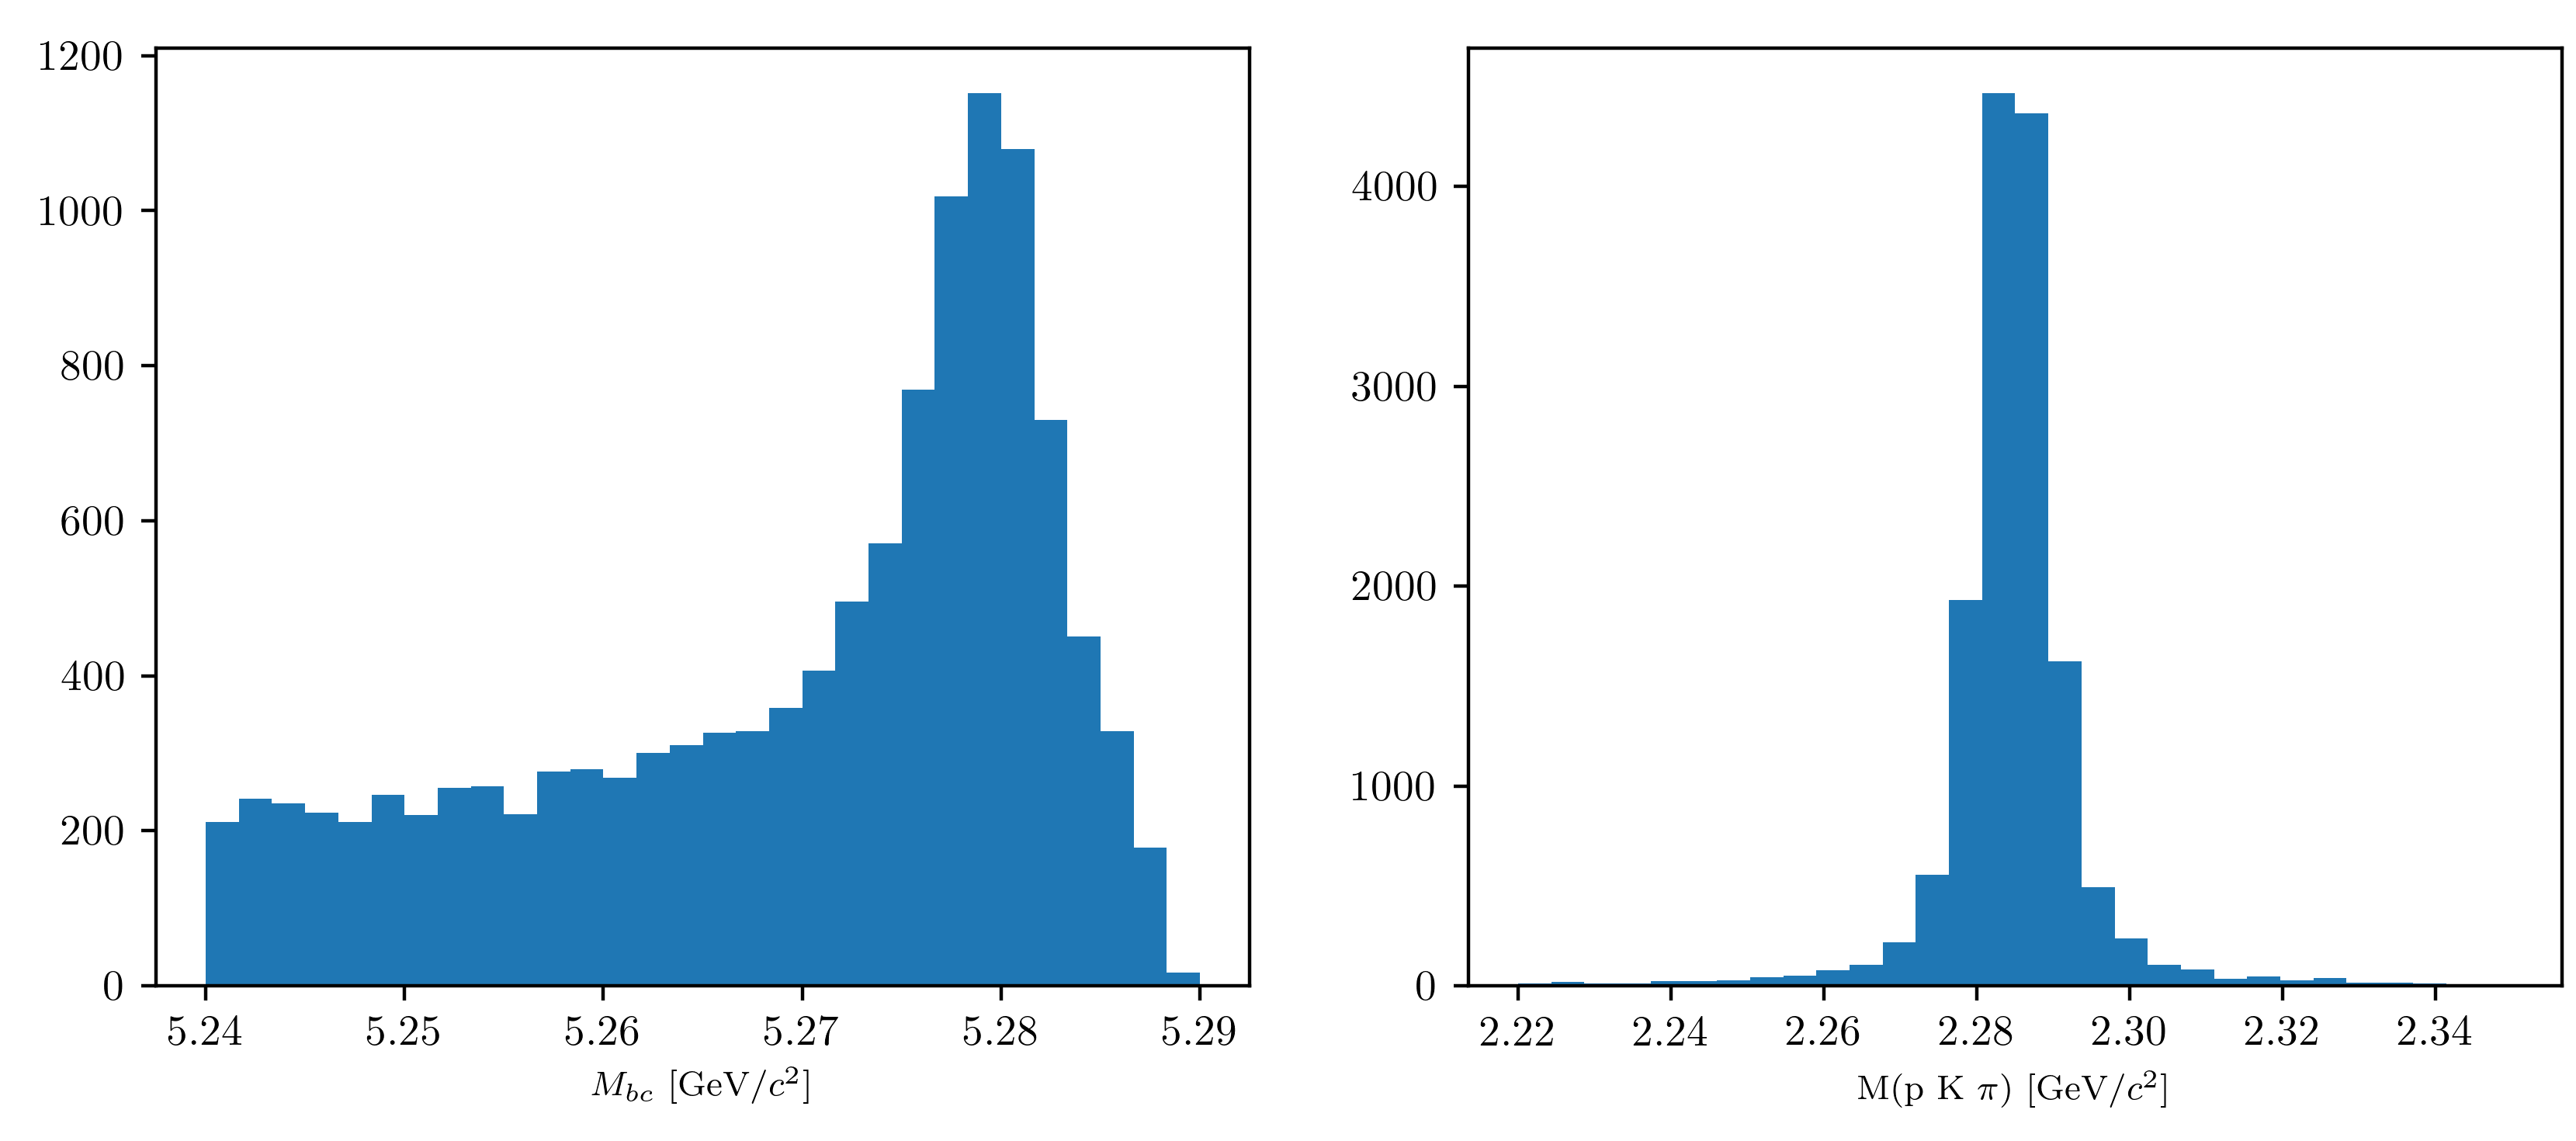
\includegraphics[width=1.0\textwidth]{03-Selection/figs/chargedBcorr_Mbc_MpKpi_TotalSignal.png}}
\caption{$M_{bc}$ and $M(p K \pi)$ distributions of $B_{tag}$ and $\Lambda_c$ candidates reconstructed in the signal sample.}
\label{fig:chargedBcorr_Mbc_MpKpi_TotalSignal}
\end{figure}

\subsection{Wrongly reconstructed $B_{tag}$ candidates}\label{wronglyBtag}

In the case of the signal sample the distributions for the beam-constrained mass $M_{bc}$ and for the correctly reconstructed $\Lambda_c$ candidates, look
like in \cref{fig:chargedBcorr_Mbc_MpKpi_TotalSignal}. If one then investigates the $M_{bc}$ distribution of the $B_{tag}$ candidates reconstructed with 
FEI, it can be seen that there is a peaking structure for wrongly reconstructed $B$ 
mesons (as in \cref{fig:wrongly_recoB}), according to the BASF2 internal truth matching variable \textbf{isSignal}.
It is obvious from this that the BASF2 internal truth matching variable cannot be used to separate properly the signal events in correctly and wrongly reconstructed $B$ mesons. In the study  BELLE2-NOTE-TE-2021-026 \url{https://docs.belle2.org/record/2711/files/BELLE2-NOTE-TE-2021-026.pdf} a possible solution was found developing new variables that can be used for an improved truth matching for the FEI (those variables were added to a newer BASF2 release than the one used for this study). In the present study instead a more "traditional" approach was adopted: fitting the $M_{bc}$ distribution with a sum of PDFs that account for the flat (background) component and the peaking (signal) component. The first component represents the combinatorial background, i.e. $B$ mesons that were mis-reconstructed, and therefore those events are denoted from now on as    "\textbf{misreconstructed signal}".  
The peaking component represents the correctly reconstructed signal events in $M_{bc}$ and therefore denoted from now on as "\textbf{reconstructed signal}".  Only the second one is then considered for the signal yield, while the first is counted as a background.
To validate this method a control decay study was performed on the flavor correlated $B^+ \rightarrow \bar{D^0}$ channel. 


\begin{figure}[h!]
\centering
{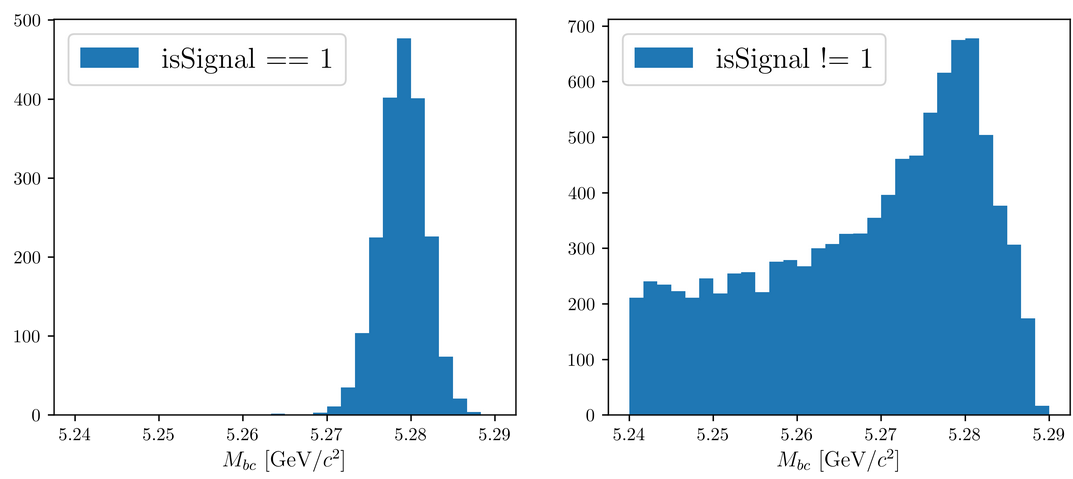
\includegraphics[width=1.\textwidth]{03-Selection/figs/wrongly_recoB.png}}
\caption{$M_{bc}$ distribution of $B_{tag}$ candidates reconstructed in the signal sample, truth-matched (on the left) and not (on the right).}
\label{fig:wrongly_recoB}
\end{figure}



\section{Signal selection optimization}

To further enhance the purity of the signal decays, an optimization procedure is adopted to determine optimal cuts for a set of variables for each decay mode under investigation by this study.
The cuts on the following variables are optimized:
\begin{itemize}
    \item $foxWolframR2$: the event based ratio
of the 2-nd to the 0-th order Fox-Wolfram moments
    \item SignalProbability: the already mentioned signal probability calculated by FEI using FastBDT
    \item $p^{\Lambda_c}_{CMS}$: momentum of the $\Lambda_c$ candidates in the center of mass system
\end{itemize}

The optimization is based on the Figure Of Merit (FOM): FOM = $\frac{S}{\sqrt{S+B}}$

Where S and B are respectively signal and background events in the signal region: $M_{bc} > $ 5.27 GeV/$c^2$,  2.2665  $< M(p K \pi) <$ 2.3065 GeV/$c^2$.\\
Due to the issue reported in Sec. \ref{wronglyBtag}, to separate signal events that peak in $M_{bc}$ from the ones that are not (which are then categorized as background events), the events reconstructed in the signal sample are fitted. with a sum of Crystal Ball function and Argus for each cut value on the corresponding variable to optimize (as in \cref{fig:wrongB_Mbc}).

\begin{figure}[h!]
%\centering
{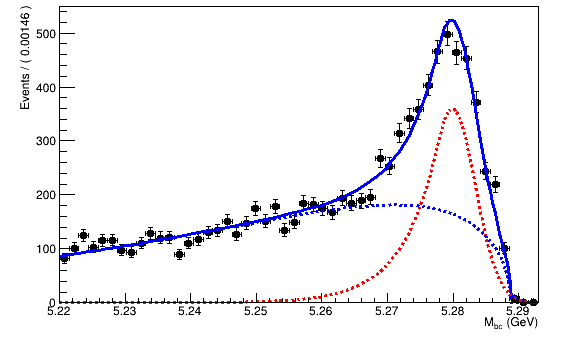
\includegraphics[width=0.75\textwidth]{03-Selection/figs/wrongB_Mbc.png}}
\caption{Example of a fit used to separate the correctly reconstructed $B$ mesons (described by the red dotted Crystal Ball function) from the wrongly reconstructed ones (described by the blue dotted Argus function).}
\label{fig:wrongB_Mbc}
\end{figure}


\include{04-chargedCorrBtoLambda/chargedCorrBtoLambda}
%!TEX root = ../main.tex

\section{$B^- \rightarrow D^0$ control decay}
\label{sec:chargedCorrBtoD0}

To monitor the analysis steps, which are applied to both measured and simulated data, a control decay of the form \\
%\vspace{0.1 cm}\\
\begin{center}
 $B^+ \rightarrow D^0 X$, $D^0 \rightarrow K^+ \pi^-$ 
\end{center}
%\vspace{0.1 cm}
is used. The statistics is much more abundant for this channel.

\subsection{Dataset used}

For this analysis the amount of data and Monte Carlo simulated data used was restricted to the SVD2 period: experiments ranging from 31 to 65. This choice was made to save processing time, anyway most of the $B\bar{B}$ meson pairs were produced in this range of experiments (620 $\times 10^6$ out of almost 800 $\times 10^6$ ).

\subsection{Event selection and reconstruction}

The approach used for the inclusive decays reconstruction is the same as for the $B \rightarrow \Lambda_c$ analysis. The same FEI training was used, though excluding the signal decay $D^0 \rightarrow K^+ \pi^-$ from the decay chains used by the FEI to reconstruct the $B_{tag}$.
Same preliminary selection criteria were applied to the tag-side $B$ meson candidates as well. \\
\noindent In the \textit{rest of event} (ROE) of the reconstructed $B_{tag}$ meson, to select $D^0 \rightarrow K^+ \pi^-$ signal candidates, the following event selection criteria are applied:
\begin{itemize}
\item $dr <$ 2 cm and $|dz| <$ 4 cm
\item $\frac{\mathcal{L}_{K}}{\mathcal{L_{K}}+\mathcal{L_{\pi}}} > 0.6$
\end{itemize}
For the $D^0 $ candidates a vertex fit is performed with \texttt{TreeFitter}, requiring it to converge.  If there are more than one $D^0$ combination, then the best candidate based on the $\chi^2$ probability is chosen. The $D^0$ signal region is defined to be $|M_{D^0}  - m_{D^0}| < $   30  MeV/$c^2$ 
\newline \noindent ($\sim$ 3$\sigma$), where $m_{D^0 }$ is the nominal mass of $D^0$.\\
\subsection{Signal selection optimization}\label{Sec:SigSelectionOpt}

Following the same procedure as for the $B \rightarrow \Lambda_c$ analysis, the optimized selection cuts obtained for the event based ratio
of the 2-nd to the 0-th order Fox-Wolfram moments, the $B_{tag}$ signal probability and the momentum of the $D^0$ candidates in the center of mass system are\footnote{illustrative plots can be found in Appendix \ref{chargedBtoD0App}}:
\begin{itemize}
\item $foxWolframR2 <$ 0.3
\item SignalProbability $>$ 0.004
\item $p^{D^0 }_{CMS} > 1$ GeV/c$^2$
\end{itemize}

 \noindent Figure \ref{fig:chargedControlD0_Mbc_InvM_opt_SignalRegion} shows the distributions of $M_{bc}$ and invariant mass in the signal region\footnote{signal region: $M_{bc}  > $ 5.27 GeV/c$^2$ and $|M_{D^0}  - m_{D^0}| < $   30  MeV/$c^2$}  for the $B^- \rightarrow D^0 X$ reconstructed events after the selection cuts were applied.

\begin{figure}[h!]
\centering
{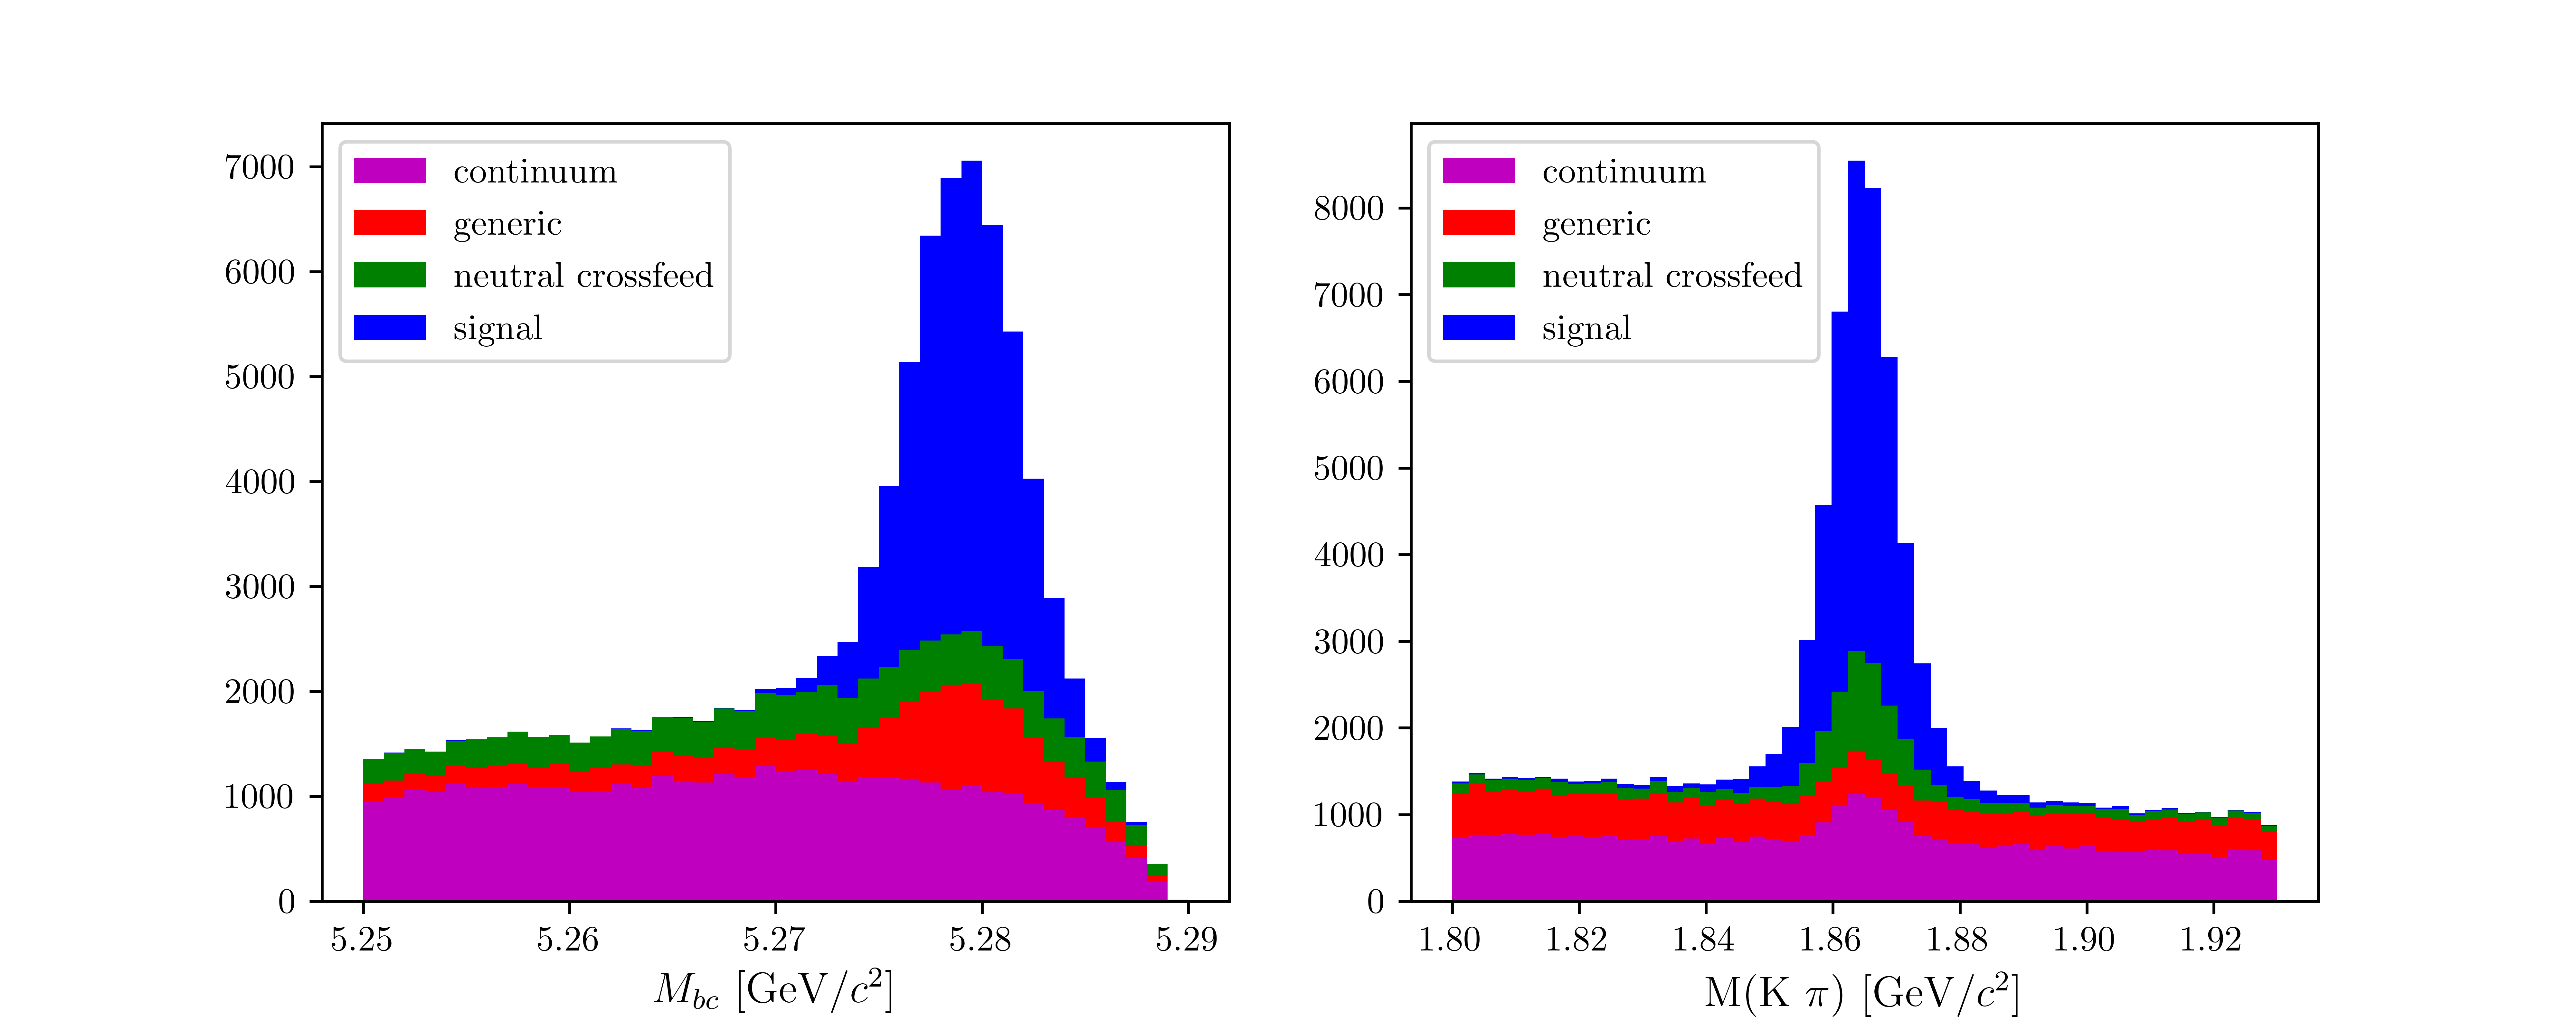
\includegraphics[width=1.2\textwidth]{05-chargedControlSample/figs/rel5_chargedBtoD0bar_Mbc_InvM_opt_SigRegion.png}}
\caption{Distribution of $M_{bc}$ (left) and invariant mass of charged correlated  $D^0 $ candidates (right), in the signal region after the above mentioned selection cuts.}
\label{fig:chargedControlD0_Mbc_InvM_opt_SignalRegion}
\end{figure}

\vspace{1 cm}

\subsection{Probability Density Functions (PDFs) for two dimensional fit}

As already said the main goal of the control sample analysis is to ensure that the method used to extract the signal yields discriminating the correctly reconstructed from the misreconstructed signal events by fitting is valid.
The reconstructed events in $M_{bc}$ are fitted with a Crystal Ball, the misreconstructed signal with a Novosibirsk function. As in the $B \rightarrow \Lambda_c$ analysis both components have a correspondent peak in the $D^0$ mass which 
is fitted with a sum of three gaussians with a common mean.
The fitted distribution of $M_{bc}$ and $M(\pi K)$ are shown in Fig. \ref{fig:chargedTotalSignal2Dfit} with signal MC sample. 

\begin{figure}[H]
%\centering
{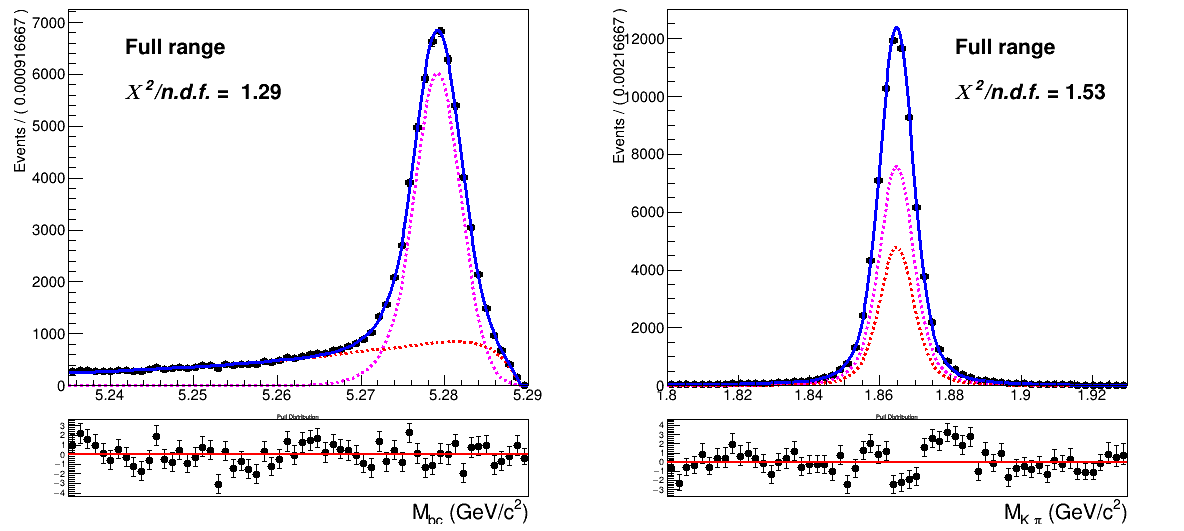
\includegraphics[width=0.90\textwidth]{05-chargedControlSample/figs/TotalSignal2Dfit_Mbc_free_Novosibirsk_and_CB_w_sig_frac.png}}
\caption{Two dimensional fit of total signal events in $M_{bc}$  and $M(p K \pi)$ (in magenta reconstructed signal PDF, misreconstructed signal PDF in red)}
\label{fig:chargedTotalSignal2Dfit}
\end{figure}

As already seen in the $B \rightarrow \Lambda_c$ analysis  besides the misreconstructed signal the other background components are:

\begin{itemize}
    \item \textbf{generic} (charged $B$) background
    \item \textbf{crossfeed} (neutral $B$) background 
    \item \textbf{continuum} background 
\end{itemize}
\vspace{0.2 cm}
\noindent \textbf{Generic background}

\noindent The generic background deriving from other $B^+B^-$ events presents a similar shape in $M_{bc}$: it is fitted again with a sum of Crystal Ball and Novosibirsk function. Instead the distribution in  the $D^0$ mass  is fitted with a sum of first order Polynomial function and a small gaussian peak, which is due to the small 
amount of flavor anti-correlated $B^+ \rightarrow D^0$ reconstructed events (see Fig. \ref{fig:chargedControlD0_Generic_2DFit}). The total two-dimensional PDF is a product of the one-dimensional PDFs in $M_{bc}$ and $D^0$ mass:

\begin{equation}
P^{GenBkg}_{B,D^0}(M_{bc}, M(K \pi)) = [\Gamma_{CB}(M_{bc}) + \Gamma_{Nov}(M_{bc})] \times [\rho_{pol1}(M(K \pi)+ \rho_{G}(M(K \pi))
 \end{equation}



\begin{figure}[H]
%\centering
{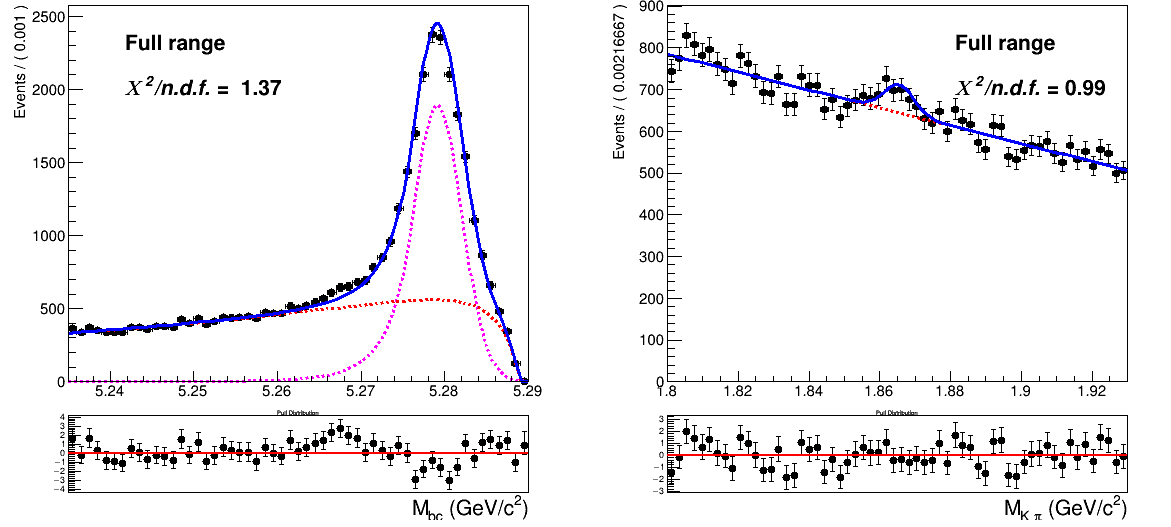
\includegraphics[width=0.90\textwidth]{05-chargedControlSample/figs/chargedControlD0_Generic_2DFit.png}}
\caption{Two dimensional fit of generic ($B^+B^-$) background events in $M_{bc}$  and $M(K \pi)$.}
\label{fig:chargedControlD0_Generic_2DFit}
\end{figure}

\noindent \textbf{Crossfeed background}
\noindent The crossfeed background deriving from $B^0\bar{B^0}$ events is shown in Fig. \ref{fig:chargedControlD0_NeutralCrossfeed_2DFit} 
The $M_{bc}$  distribution is fitted with a sum of Novosibirsk and Argus functions.
The distribution in the $D^0$ mass is fitted with a first order Chebyshev polynomial and the $D^0$ mass peak is fitted with the same sum of three gaussians used to describe the signal peak (same parametrization used already in $\BtoLambda$ analysis).

\begin{figure}[h!]
{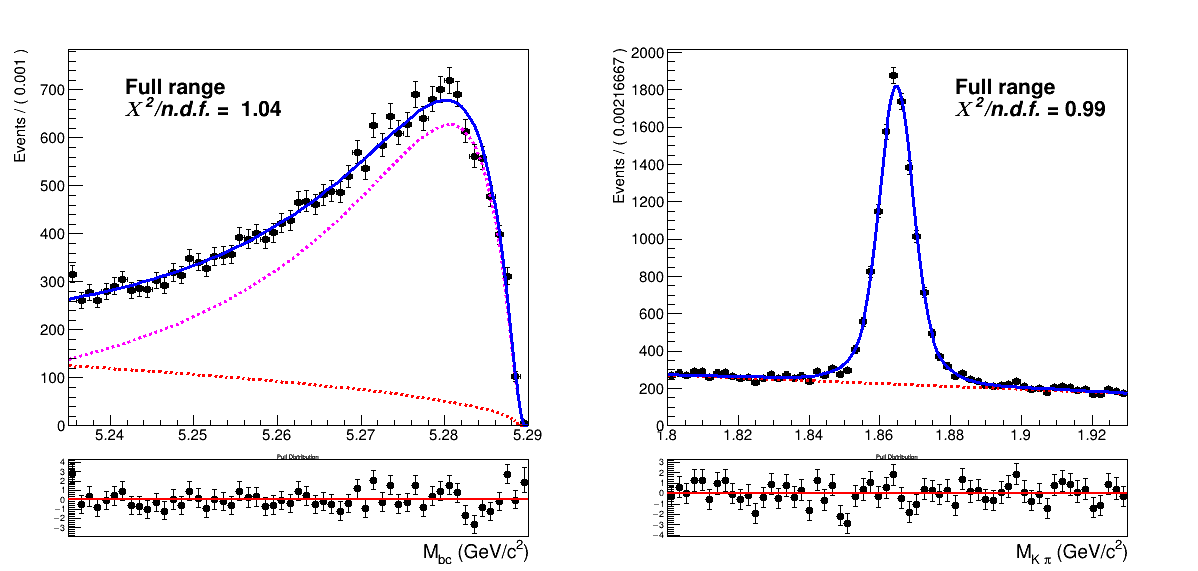
\includegraphics[width=0.90\textwidth]{05-chargedControlSample/figs/NEW_chargedControlD0_NeutralCrossfeed_2DFit_.png}}
\caption{Two dimensional fit of crossfeed ($B^0\bar{B^0}$) events in $M_{bc}$  and $M(K \pi)$.}
\label{fig:chargedControlD0_NeutralCrossfeed_2DFit}
\end{figure}

\noindent \textbf{Continuum background}
\newline
\noindent The procedure adopted to model the continuum background is the same used for the $B \rightarrow \Lambda_c$ decays, but in this case
the available statistics is enough to perform the scaling with all the selection cuts also in the case of the two-dimensional fit (not removing the continuum suppression).

  
 \begin{figure}[H]
 \centering
\subcaptionbox{\label{fig:chargedControlD0_2Dcontinuum_on-offMbc}}
{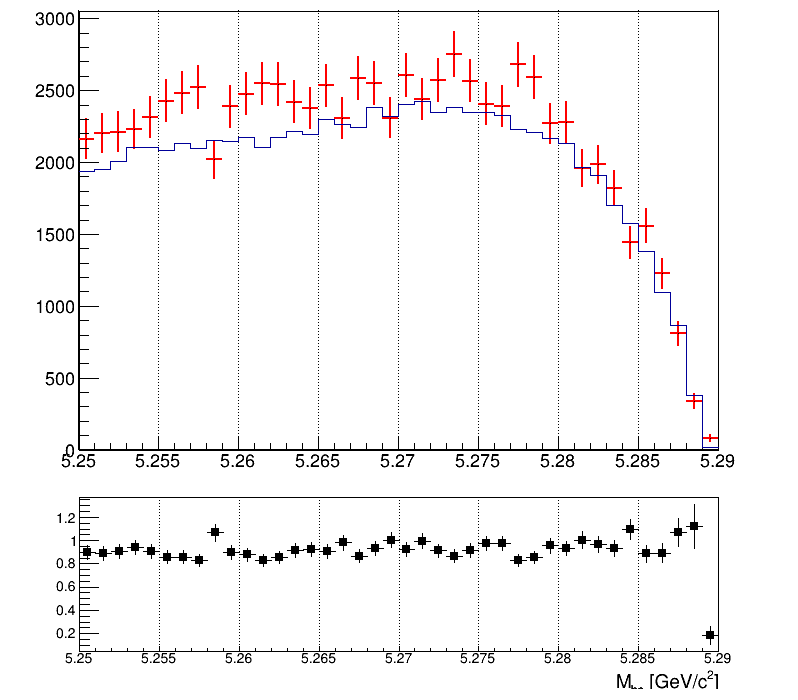
\includegraphics[width=.45\textwidth]{05-chargedControlSample/figs/on_off_res_chargedControlD0_Mbc.png}}
\subcaptionbox{\label{fig:chargedControlD0_corrected_2DcontinuumMbc}}
{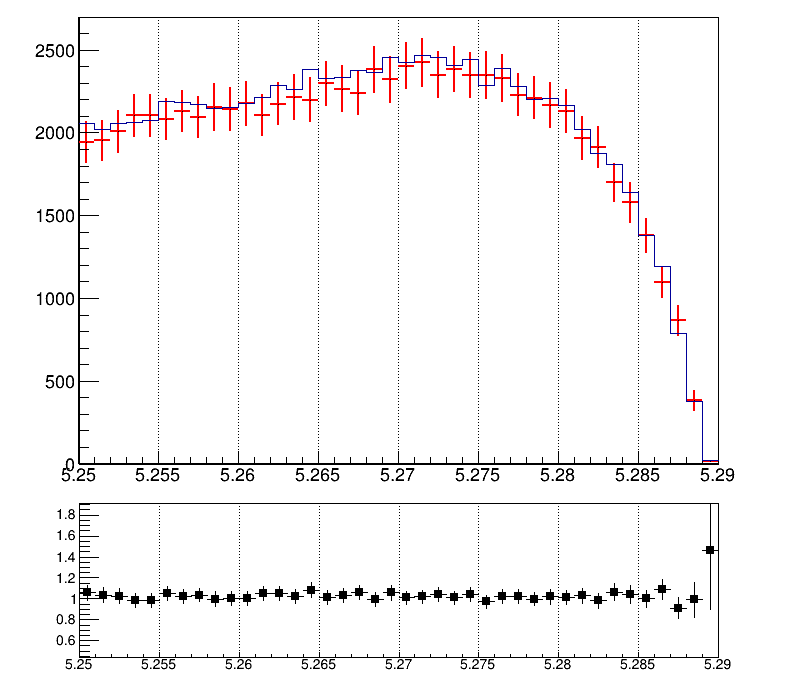
\includegraphics[width=.45\textwidth]{05-chargedControlSample/figs/chargedControlD0_corrected_2DcontinuumMbc.png}}
\caption{In \cref{fig:chargedControlD0_2Dcontinuum_on-offMbc} $M_{bc}$ distributions of the MC (scaled) off-resonance sample (in red) and on-resonance (in blue).  In \cref{fig:chargedControlD0_corrected_2DcontinuumMbc} $M_{bc}$ distributions of the corrected scaled off-resonance and on-resonance MC continuum.}
\end{figure}

\noindent For each bin a correction factor is calculated, in order to have a reasonable match with the expected continuum background. Fig. \ref{fig:chargedControlD0_corrected_2DcontinuumMbc} shows the applied correction on an independent MC sample.
As in the case of $B \rightarrow \Lambda_c$ analysis, then the resulting $M_{bc}$ distribution is fitted with a Novosibirsk function , whereas the $D^0$ mass distribution is fitted with a sum of first order Chebyshev polynomial and the sum of three gaussians used to describe the signal peak (as shown in \cref{fig:InvMchargedControlD0_off-resonanceMC_rescaled_2Dfit_w_peak_frac}). The fraction of events in the peak is the same in on- and off-resonance MC. This method is applied also to scale the off-resonance data.

\begin{figure}[H]
\centering
{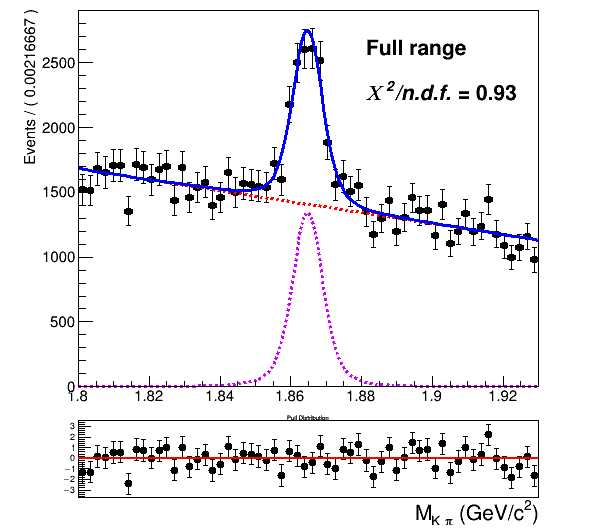
\includegraphics[width=0.40\textwidth]{05-chargedControlSample/figs/InvMchargedControlD0_off-resonanceMC_rescaled_2Dfit_w_peak_frac.png}}
\caption{$D^0$ mass fit of scaled off-resonance  Monte Carlo}
\label{fig:InvMchargedControlD0_off-resonanceMC_rescaled_2Dfit_w_peak_frac}
\end{figure}

\subsection{2D Fit on Monte Carlo simulated data}\label{2Dfit_chargedControlD0_onMC}

As in the $\BtoLambda$ study, five streams of Monte Carlo simulated data have been used to get values for the shaping parameters for the individidual components described in the previous section and the fit model is tested on 
an independent stream.
%In all six fits all the shaping parameters are kept fixed, except:
%\begin{itemize}
%    \item $\sigma_{G1}$: the width of the wider of the three Gaussian functions in $\rho_G(M(p K \pi))$
%    \item $\sigma_{CB}$ parameter for the Crystal Ball describing the signal
%\end{itemize}
 
For the six fits, the same conditions were applied to the widths:
\begin{itemize}
      \item $\sigma_{G1}$: the width of the wider of the three Gaussian functions in $\rho_G(M(K \pi))$
      \item $\sigma_{CB}$ parameter for the Crystal Ball describing the signal
      \item the $\sigma_{CB}$ parameter for the Crystal Ball describing the generic background is expressed as function of the signal $\sigma_{CB}$  with a ratio fixed from the MC. 
\end{itemize}

For the fits on Monte Carlo simulated data the crossfeed normalization is expressed as ratio of its contribution  and the misreconstructed signal as found in MC and kept fixed (to see how the parametrized form impacts a fit on data is then performed).
Exemplary, the distributions of stream 0 overlaid by the fitted PDF are depicted in \cref{fig:stream0_chargedControlD0_Total_2DFit} (see Appendix \ref{chargedBtoD0App} for the projections of signal regions and sidebands). 
%(floated parameters and fixed width ratios) were applied as to the two dimensional fit in the case of the \BtoLambda study.
%Those conditions are the same used ofr the  
 %Figures \ref{fig:stream0_chargedControlD0_Total_2DFit} - \ref{fig:stream4_chargedControlD0_Total_2DFit} show the fits of the 5 streams used to obtain the shaping parameters of the PDFs.

%\newpage 
In Table \ref{tab:5streams_chargedSignalYields} the yields for reconstructed and misreconstructed signal are listed for each stream.\\
%\vspace{0.1 cm}
\begin{table}[H]
\centering
%\resizebox{0.8\textwidth}{!}{%
\begin{tabular}{ |p{1.5cm}||p{2.2cm}| p{2.2cm}| p{2.2cm}| p{2.2cm}| p{2.2cm}| p{2.2cm}|  }
 \hline
  stream   &  0  & 1 & 2 & 3 & 4 & 5 \\
 \hline
 NrecSig  &  56986 $\pm$ 400  & 57766 $\pm$ 437  & 55607 $\pm$ 426 & 57068 $\pm$ 372 & 58385 $\pm$ 369 & 57501 $\pm$ 437 \\
 NmisSig &  31453 $\pm$ 321 & 30513 $\pm$ 350 & 32580  $\pm$ 350 & 33340 $\pm$  399 & 29966  $\pm$ 390 & 32012 $\pm$ 355\\
 %Generic & 36191 $\pm$ 436 &  33432 $\pm$ 439 & 37223 $\pm$ 446 &  37015  $\pm$ 388 & 34079  $\pm$ 382\\
 \hline
 \end{tabular}%
%}%
 \caption{reconstructed and misreconstructed signal yields obtained fitting 6 independent streams}\label{tab:5streams_chargedSignalYields}
\end{table}
%\vspace{0.5 cm}

To be sure that the PDFs enables us to extract the signal yield in an unbiased way, the sum of reconstructed and misreconstructed signal yields, i.e. total signal, from the fits are compared to the true values of each stream (\cref{tab:5streams_chargedTotalSignalYields}).
There are quite some differences between the fitted signal yield and the true values in individual streams. However,  all these deviations are within statistical expectations. \\

\vspace{0.5 cm}
%Total Signal:
\begin{table}[H]
\centering
\begin{tabular}{c c c c c}% |p{2cm}||p{2.5cm}| p{2.5cm}| p{2.5cm}| p{2.5cm}|   p{4cm}| }
 \hline
  streams   &  fit  & MC truth  &\multicolumn{2}{c}{fit - MC truth}  \\
 \hline
 stream 0 &  88439  $\pm$ 340  & 88144  & + 295 & (+0.33$\%$)  \\
 stream 1 &  88279 $\pm$ 361 & 88551 & $ - 272$ & (- 0.31$\%$)\\
 stream 2  & 88187 $\pm$ 360 &  88487 & -300 & (- 0.34$\%$)  \\
  stream 3  & 90408 $\pm$ 372 &  90149  &   + 259 & (+ 0.29$\%$) \\
   stream 4  & 88351 $\pm$ 383 &  87981  &  + 370 & (+ 0.42$\%$) \\
stream 5  & 89513 $\pm$ 366 &  89710  &  -197 & (- 0.22$\%$) \\
    \hline
     sum  & 533177  &  533022  & +155 & (+0.03$\%$)  \\  
 \hline 
\end{tabular}
\caption{Comparison of fitted and truth-matched total signal events in each stream.}\label{tab:5streams_chargedTotalSignalYields}
\end{table}


\begin{figure}[H]
\centering
{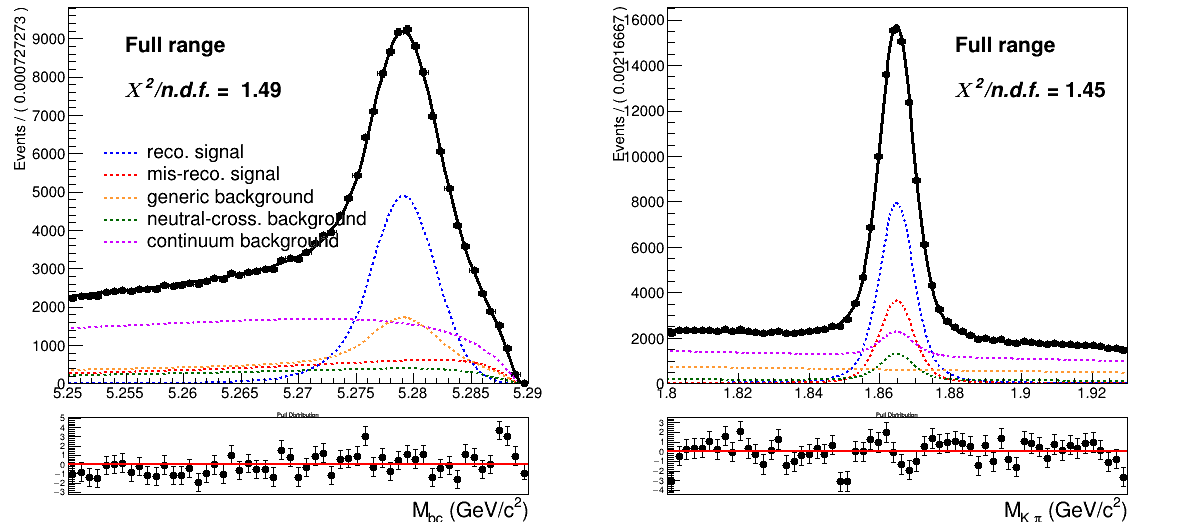
\includegraphics[width=0.85\textwidth]{05-chargedControlSample/figs/stream0_chargedControlD0_Total_2DFit.png}}
\caption{Two dimensional fit on stream 0 Monte Carlo simulated data.}
\label{fig:stream0_chargedControlD0_Total_2DFit}
\end{figure}

\subsection{2D Fit on data}\label{chargedBtoD0_2Dfit_onData}
 After obtaining the model for the continuum background scaling and correcting the $M_{bc}$ distribution of the off-resonance data, the model tested on Monte Carlo simulated data is applied on data with same free parameters and yields. \cref{fig:chargedControlD0_Total_2DFit_onData_free_sigmaCB1_InvMsigma} shows the projections of the two dimensional fit (see Appendix \ref{chargedBtoD0App} for the projections of signal regions and sidebands).
\begin{figure}[h!]
%\centering
{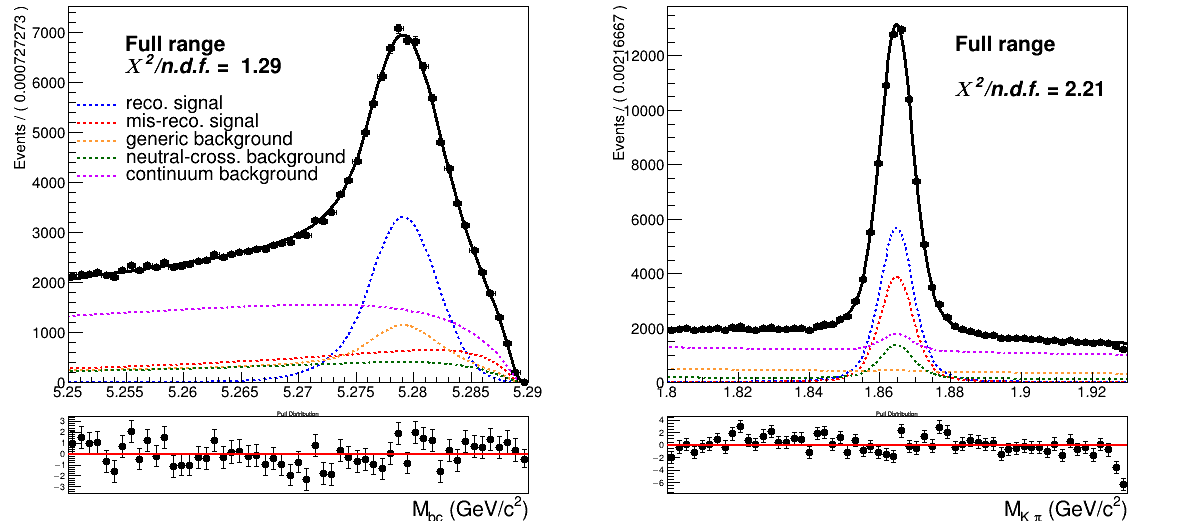
\includegraphics[width=0.80\textwidth]{05-chargedControlSample/figs/chargedControlD0_Total_2DFit_onData_free_sigmaCB1_InvMsigma.png}}
\caption{Two dimensional fit on Data (same conditions applied as in \cref{fig:stream0_chargedControlD0_Total_2DFit})}
\label{fig:chargedControlD0_Total_2DFit_onData_free_sigmaCB1_InvMsigma}
\end{figure}

\noindent Yields for the reconstructed and misreconstructed signal and for generic background are obtained from the fit: \\
 .
 \newline  \hspace{3.5 cm}
\begin{tabular}{ |p{3cm}||p{3cm}|  }

 \hline
 NrecSig  &  35629 $\pm$ 368\\
 NmisSig &  24425 $\pm$ 311 \\
 Generic & 24596 $\pm$ 407\\
 \hline
\end{tabular}
\newline
\vspace{1.5 cm}

\noindent  The total normalization from the fit is 174230 $\pm$  407 (to be compared with the total data events: 173964).\\
\vspace{0.5 cm}
 \begin{table}
\begin{tabular}{ |p{3cm}||p{3cm}| p{3cm}|  }

 \hline
 ratio        &          MC      &    DATA   \\
 \hline
 \hline
NmisSig/NrecSig  &  0.56 $\pm$ 0.01  & 0.68 $\pm$ 0.01\\
NmisSig/Generic  &  0.90 $\pm$ 0.02 &  0.99 $\pm$ 0.02  \\
Generic/NrecSig & 0.62 $\pm$ 0.01 & 0.69 $\pm$ 0.02\\
 \hline

\end{tabular}
 \caption{Comparison of ratios of yields from the two dimensional fits on Monte Carlo simulated data and on Data.} 
 \end{table}

 \noindent Since in the case of the two dimensional fit for the measurement of $B^- \rightarrow \Lambda_c^+ X$ decays the crossfeed normalization was parametrized in the form described 
 by \cref{eq:paramCrossfeedNorm}, the 2D fit shown above is repeated with the parametrized normalization for the crossfeed background. The signal reconstruction efficiency  that enters the formula to estimate the true number of 
 signal events ( $ N_{sig}  =  N_{recSig} / \epsilon$ ) is now the signal reconstruction efficiency on data: $\epsilon_{data}$. It can be estimated scaling the one found on Monte Carlo by a correction factor that takes into account the different 
 FEI efficiency on data and the signal-side reconstruction corrected for the different PID efficiency (see \cref{sec:ControlPIDeff}-\cref{sec:ControlRecoEff}), $\epsilon_{data} = \epsilon_{MC} \cdot c_{FEI} \cdot c_{D^0} = (0.216 \pm 0.016)\% $. \\

 where $c_{FEI} = 0.810_{-0.012}^{+0.013} \pm 0.054$ is the correction factor for the FEI efficiency determined in \cite{schwab_judith_2017_21422} \\
 whereas the factor $c_{D^0}$ is the PID correction reported in \cref{sec:ControlPIDeff}.\\
 \noindent \cref{fig:chargedControlD0_Total_2DFit_onData_paramCrossfeedRatio} shows this second fit.
 
 \newpage
 \noindent In the following table yields for the reconstructed and misreconstructed signal and for generic background obtained from this second fit are reported: \\

\begin{tabular}{ |p{3cm}||p{3cm}|  }

 \hline
 NrecSig  &  36553 $\pm$ 360\\
 NmisSig &  24115 $\pm$ 283 \\
 Generic & 25900 $\pm$ 409\\
 \hline
\end{tabular}

 \begin{figure}[H]
  %\centering
  {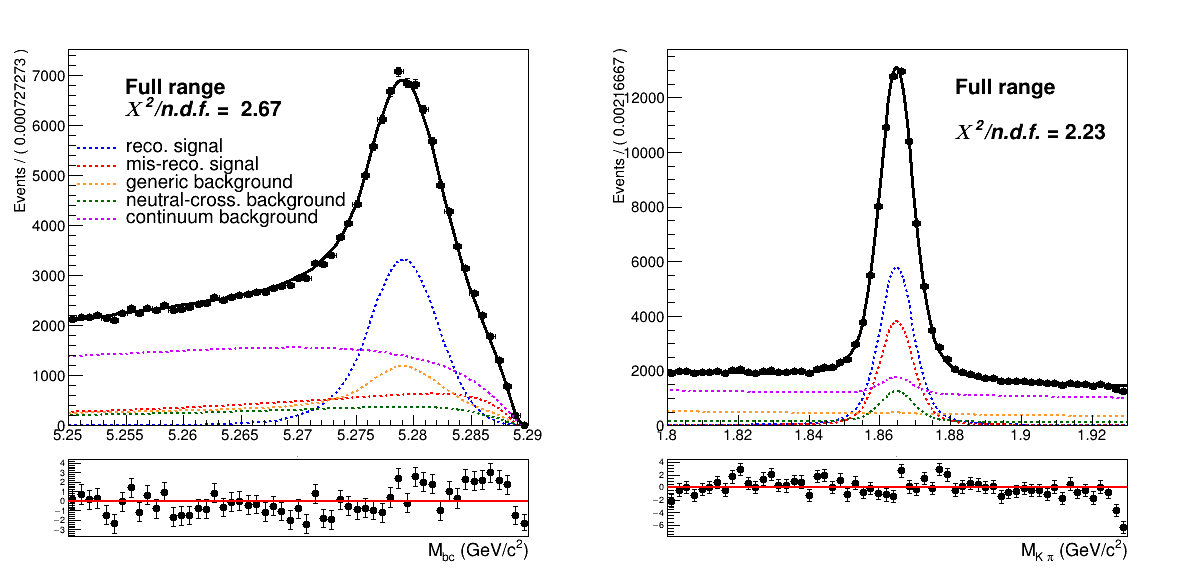
\includegraphics[width=0.80\textwidth]{05-chargedControlSample/figs/chargedControlD0_Total_2DFit_onData_paramCrossfeedRatio.png}}
  \caption{Two dimensional fit on Data with parametrized normalization of crossfeed background}
  \label{fig:chargedControlD0_Total_2DFit_onData_paramCrossfeedRatio}
  \end{figure}
 

  \vspace{0.5 cm}
  \begin{table}
 \begin{tabular}{ |p{3cm}||p{3cm}| p{3cm}|  }
 
  \hline
  ratio        &          MC      &    DATA   \\
  \hline
  \hline
 NmisSig/NrecSig  &  0.56 $\pm$ 0.01  & 0.66 $\pm$ 0.01\\
 NmisSig/Generic  &  0.90 $\pm$ 0.02 &  0.93 $\pm$ 0.02  \\
 Generic/NrecSig & 0.62 $\pm$ 0.01 & 0.71 $\pm$ 0.02\\
  \hline
 
 \end{tabular}
  \caption{Comparison of ratios of yields from the two dimensional fits on Monte Carlo simulated data and on Data (from the fit shown in \cref{fig:chargedControlD0_Total_2DFit_onData_paramCrossfeedRatio}).} 
  \end{table}




\newpage 
\subsection{Probability Density Functions (PDFs) for the $B_{tag}$}
Like for the signal model in the 2D fit the $M_{bc}$ distribution of the tagged charged $B$ mesons is fitted with a Crystal Ball as for the reconstructed  signal component, whereas the misreconstructed signal component is fitted with a Novosibirsk function (Fig. \ref{fig:stream0_chargedBtagFit_400bins_fixed_old_parameters_freeSigmaCB_and_misRecoPdf}).

\begin{figure}[H]
\begin{minipage}{.5\textwidth}
\centering
\subcaptionbox{\label{fig:stream0_chargedBtagFit_400bins_fixed_old_parameters_freeSigmaCB_and_misRecoPdf}}
{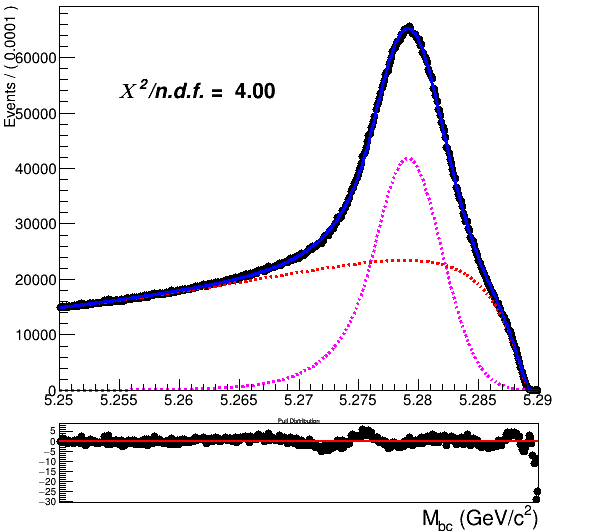
\includegraphics[width=0.80\textwidth]{05-chargedControlSample/figs/stream0_chargedBtagFit_400bins_fixed_old_parameters_freeSigmaCB_and_misRecoPdf.png}}
\end{minipage} 
 \begin{minipage}{.5\textwidth}
\subcaptionbox{\label{fig:NeutralCrossfeed_stream0_ControlD0_chargedBtag_MbcFit}}
{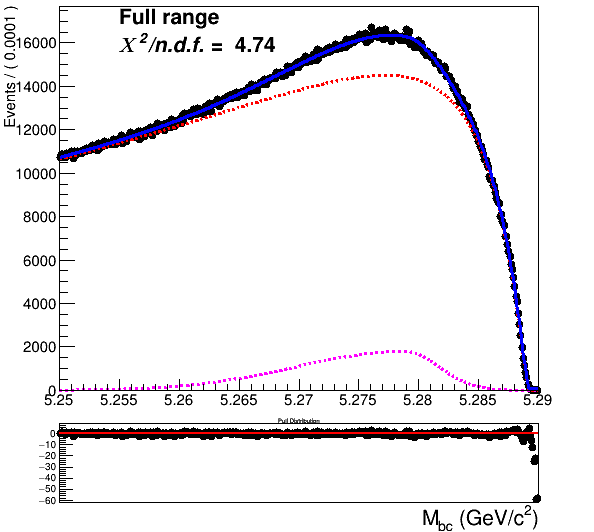
\includegraphics[width=0.80\textwidth]{05-chargedControlSample/figs/NeutralCrossfeed_stream0_ControlD0_chargedBtag_MbcFit.png}}
\end{minipage}
\caption{On the left: fitted distribution of tagged charged $B$ mesons, reconstructed signal events (magenta) are described by a Crystal Ball whereas the misreconstructed signal events (red) are described by a Novosibirsk function. On the right: Crossfeed distribution fitted with a sum of Novosibirsk (red) and asymmetric Gaussian PDF (magenta)}
\end{figure}


\noindent The crossfeed background is fitted instead with a sum of a Novosibirsk and an asymmetric Gaussian PDF (Fig. \ref{fig:NeutralCrossfeed_stream0_ControlD0_chargedBtag_MbcFit}).\\
\vspace{0.05 cm}

\noindent Regarding the continuum background component, same procedure used for the 2D fit was applied to the $M_{bc}$ distribution of the continuum background in this case (see Fig. \ref{fig:bin_corrected_stream1_off-resonance_on_stream3_on-resonance} for the result).

\begin{figure}[H]
\begin{minipage}{.5\textwidth}
  \centering
  {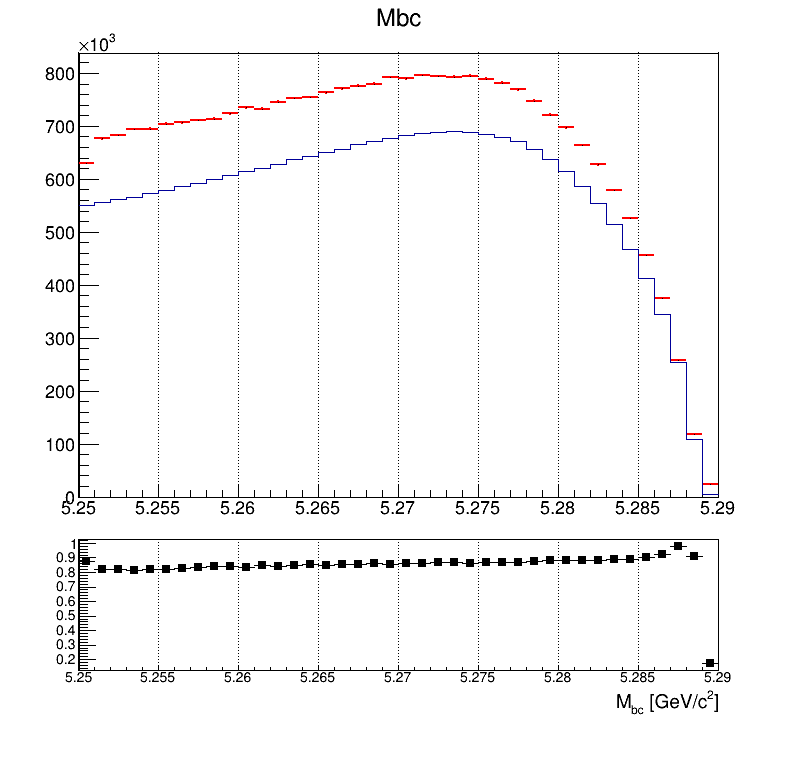
\includegraphics[width=0.80\textwidth]{05-chargedControlSample/figs/NEWstream0_chargedBtag_rescaled_off-on_resonance.png}}
%\caption{}
%\label{fig:NEWstream0_chargedBtag_rescaled_off-on_resonance}
\end{minipage}%
\begin{minipage}{.5\textwidth}
%\centering
{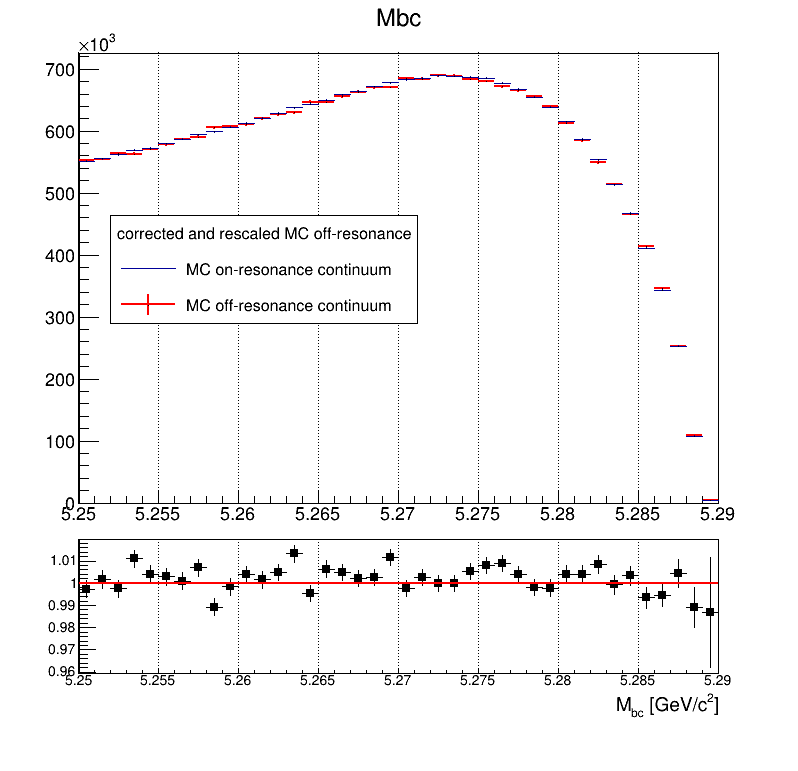
\includegraphics[width=0.80\textwidth]{05-chargedControlSample/figs/bin_corrected_stream1_off-resonance_on_stream3_on-resonance.png}}
%\caption{}
\label{fig:bin_corrected_stream1_off-resonance_on_stream3_on-resonance}
\end{minipage}
\caption{On the left: $M_{bc}$ distributions of the MC off-resonance sample and the MC continuum sample. On the right: $M_{bc}$ distributions of the corrected scaled MC off-resonance and on-resonance MC continuum.}
\end{figure}


\subsection{$B_{tag}$ Fit on Monte Carlo simulated data}

An independent Monte Carlo stream was used to test the total fit model on tagged $B$ mesons candidates. 
The usual condition is applied to the crossfeed background events: the ratio between its contribution and misreconstructed signal events is fixed from the other Monte Carlo stream.\\
In this fit the shaping parameters that are not kept fixed are the Crystal Ball width ($\sigma_{CB}$) and the width of the Novosibirsk function describing the misreconstructed signal events.
As in the case of $B_{tag}$ fit in Sec. \ref{BtagFit} the range for the fit is restricted to values betweeen 5.250 and 5.287 GeV/$c^2$.   





\begin{figure}[H]
\begin{minipage}{.5\textwidth}
  \centering
  {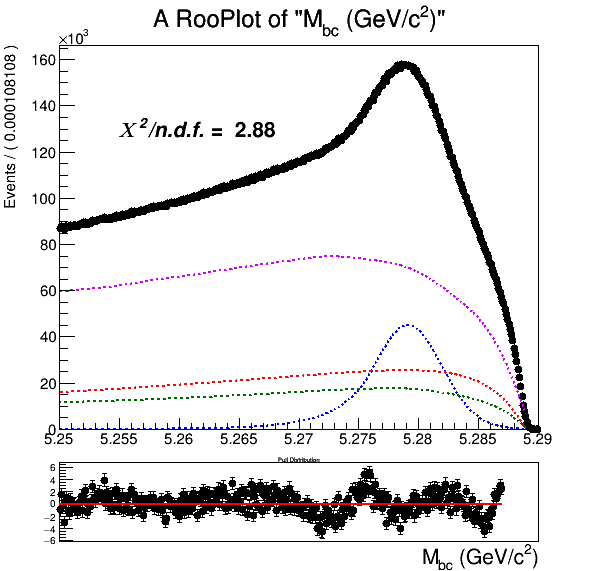
\includegraphics[width=0.95\textwidth]{05-chargedControlSample/figs/stream3_chargedBtag_Total_fit_sigmaCB_misRecSigma_free_370bins.png}}
%\caption{}
%\label{fig:NEWstream0_chargedBtag_rescaled_off-on_resonance}
\end{minipage}%
\begin{minipage}{.5\textwidth}
%\centering
{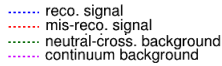
\includegraphics[width=0.55\textwidth]{05-chargedControlSample/figs/legend.png}}
%\caption{}
%\label{fig:bin_corrected_stream1_off-resonance_on_stream3_on-resonance}
\end{minipage}
\caption{Total fit of tagged $B$ mesons}
\end{figure}


Yields for the reconstructed and misreconstructed signal are obtained from the fit:

\vspace{0.5 cm}
\begin{tabular}{ |p{2cm}||p{3.8cm}|  }

 \hline
 NrecSig  & 3.25110$\cdot$10$^6 \pm$ 6759\\
 NmisSig &  7.41107$\cdot$10$^6 \pm$ 5341 \\
 \hline
\end{tabular}



\vspace{0.5 cm}
\noindent  One can then compare the  sum  NrecSig+NmisSig (the so called total signal) with the true value known from the Monte Carlo and the same for the total number of events in this particular stream: \\
 %The Total normalization from the fit is 38600851 $\pm$  6886 (to be compared with 38609945 from the Monte Carlo).


\begin{tabular}{ |P{3cm}||P{4cm}|P{2cm}|  }

\hline
      & fit & MC value\\
 \hline
 Total Signal  & 10.662$\cdot$10$^6$ $\pm$ 5249 & 10.671$\cdot 10^6$ \\
 Total events &  38.601$\cdot$10$^6$ $\pm$ 6886 & 38.610$\cdot 10^6$\\
 \hline
\end{tabular}
\vspace{0.75 cm}
\newline
\noindent The discrepancy in the total signal events from the fit and the MC here is about 1.7$\sigma$, but the relative error is an order of magnitude smaller than the one found in $B_{tag}$ fit in \ref{BtagFit} (below the \textperthousand level), therefore it's negligible.

\newpage

\subsection{$B_{tag}$ Fit on data}
The fit model tested on Monte Carlo simulated data is then applied with the same method on data \cref{fig:chargedControlD0Btag_Total_fit_onData}.

\begin{figure}[H]
\centering
{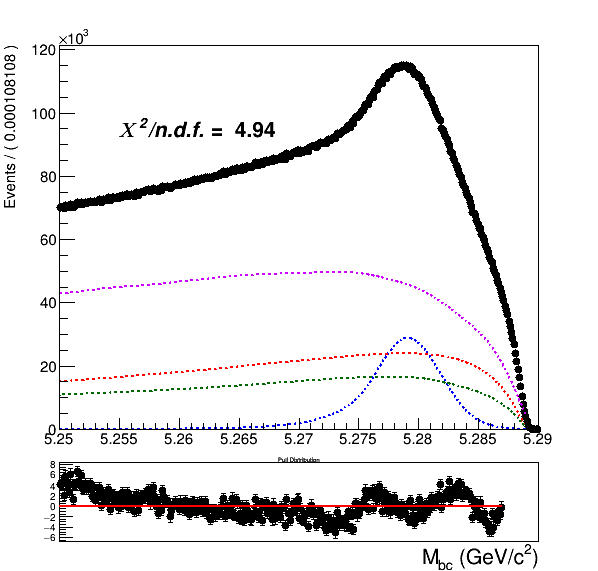
\includegraphics[width=0.40\textwidth]{05-chargedControlSample/figs/chargedBtag_Total_fit_onData_sigmaCB_free_370bins.png}}
\caption{Total fit of tagged $B^+$ mesons candidates on data}
\label{fig:chargedControlD0Btag_Total_fit_onData}
\end{figure}


Yields for the reconstructed and misreconstructed signal are obtained from the fit:

\vspace{0.5 cm}
\begin{tabular}{ |P{3cm}||P{4cm}|  }

 \hline
 NrecSig  & 2.011$\cdot$10 $^6 \pm$ 5858\\
 NmisSig &  6.975$\cdot$10 $^6 \pm$ 4667 \\
Total Signal &  8.982$\cdot$10 $^6 \pm$4587             \\
 \hline
\end{tabular}

  \vspace{0.5 cm}
  \begin{table}[H]
 %     \centering
\begin{tabular}{ |p{3cm}||p{3cm}|  p{3cm}| }

 \hline
 ratio        &          MC      &    DATA   \\
 \hline
NmisSig/NrecSig  &  2.28 $\pm$ 0.01  & 3.47 $\pm$ 0.01\\
 \hline  
 \end{tabular}
 \caption{Comparison of ratios of yields from the tagged $B$ mesons fits on Monte Carlo simulated data and on Data.}
\end{table}
 
\newpage

 \subsection{PID efficiency correction}\label{sec:ControlPIDeff}

The PID selection is applied only to Kaons: $\frac{\mathcal{L}_{K}}{\mathcal{L_{K}}+\mathcal{L_{\pi}}} > 0.6$ 
%The kaon identification efficiency  was studied in detail Belle Note 779 (\url{http://belle.kek.jp/secured/belle_note/gn779/bn779.ps.gz}). The decay $D^{*+} \rightarrow D^0 \pi^+$ followed by $D^0 \rightarrow K^- \pi^+$, was used to examine the Kaon identification efficiency difference between data and MC in \textit{Belle}.
%The efficiency ratio dependence on Kaon charge, momentum and polar angle is considered. 
%As already The Kaon ID efficiency is defined as\\

%\vspace{0.2cm}
%\hspace{3 cm}    $\epsilon_{KID} = \frac{\text{number of}\hspace{0.05 cm}K \text{tracks identified as} \hspace{0.05 cm} K}{\text{number of }K \hspace{0.05 cm} \text{tracks} }$\\

%\vspace{0.2cm}
% and the comparison between MC efficiency and data efficiency by a double ratio defined as \\

%\vspace{0.2cm} \hspace{1 cm}  $ R = \epsilon^{data}/\epsilon^{MC}$ \\

\vspace{0.5cm}
Using the values provided in the global tag \texttt{BellePID} (as done in the $\BtoLambda$ study), the average Kaon ID correction for this analysis is estimated to be $R = 0.976 \pm 0.008$.



\subsection{$D^0$ and FEI efficiency}\label{sec:ControlRecoEff}

The efficiency in reconstructing the $D^0$ after correctly tagging the charged $B$ meson, can be estimated from the 2D fit on Monte Carlo simulated data, using the reconstructed signal yield and from a sample of $B_{tag}$ candidates reconstructed in signal events in the Monte Carlo: where from $B^+ B^-$ at least a $D^0$ decaying into $\pi K$ is produced.

For the latter a fit is performed to extract the yield of correctly tagged $B$ mesons (Fig. \ref{fig:stream0_chargedBtagSignal_fit})
\begin{figure}[H]
\centering
{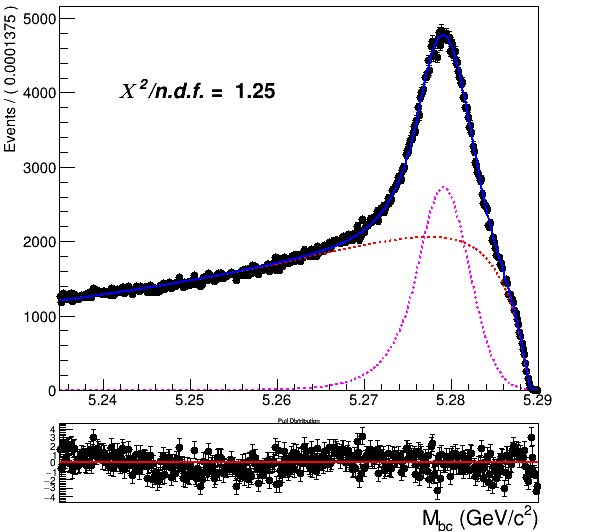
\includegraphics[width=0.40\textwidth]{05-chargedControlSample/figs/stream0_chargedBtagSignal_fit.png}}
\caption{Fit of tagged $B$ mesons in the "signal events" sample}
\label{fig:stream0_chargedBtagSignal_fit}
\end{figure}

Yields for the reconstructed and misreconstructed signal :

\vspace{0.5 cm}
\begin{tabular}{ |P{2cm}||P{4cm}|  }

 \hline
 NrecSig  & 1.46779$\cdot$10 $^5 \pm$ 767\\
 NmisSig &  6.16717$\cdot$10 $^5 \pm$ 1028 \\
 \hline
\end{tabular}
\vspace{0.5 cm}

\noindent From this and the results listed in Sec. \ref{2Dfit_chargedControlD0_onMC} 
the efficiency to reconstruct $D^0$ is obtained : \\

$\epsilon_{D^0} = \frac{NrecSig(2D) }{NrecSig((B_{tag}^{sig}} = 39.1 \pm 0.4 \%\footnote{the error reflects the limited Monte Carlo statistics}$  \hspace{0.4cm} (KID efficiency corrected value for data: 38.2 $\%$)\\
\vspace{0.2 cm}

\noindent The results from the fit shown in  (Fig. \ref{fig:stream0_chargedBtagSignal_fit}) can be used also to calculate the FEI tag-side efficiency for signal events, i.e. the efficiency to tag the $B$ meson accompanying a $B_{sig}$ decaying into a $D^0 $ on the signal side.
Whereas results from the fit  of charged $B_{tag}$ shown in Fig. \ref{fig:stream0_chargedBtagFit_400bins_fixed_old_parameters_freeSigmaCB_and_misRecoPdf} can be used to calculate the hadronic tag-side efficiency in the generic $B^+B^-$ events case.

\noindent The ratio of the two efficiencies is found to be:   $\frac{\epsilon^{+}_{FEI,  sig}}{\epsilon^{+}_{FEI}} = 1.50 \pm 0.01 $ \\
\vspace{0.2 cm}

\subsection{Studies of Systematic Effects}\label{sec:chargedControlSys}

The systematic uncertainties are studied the same way as in the case of the $B^+ \rightarrow \bar{\Lambda}_c^- X$ branching fraction. 
The values are reported in the next section. The dominant systematic uncertainty is the one originated by the continuum background modeling and its incidence in terms of relative error on the branching fraction value is same as for the $B^+ \rightarrow \bar{\Lambda}_c^- X$ study.
For this control sample study the uncertainty that would be caused by the uncertainty of the crossfeed peaking events is not estimated, since 
the uncertainty on   $\mathcal{B}(B^0 \rightarrow \bar{D^0} + X)$ is only of few percent and the possible effect can be considered negligible compared to the other systeamtic uncertainties. 


\subsection{Measured $B^+ \rightarrow \bar{D}^0 X$ inclusive Branching Fraction}\label{sec:chargedControlBRvalues}
The inclusive branching fraction of $B^+  \rightarrow \bar{D}^0 X$ can be determined by: 

\begin{equation}
    Br(B^+ \rightarrow \bar{D}^0) = \frac{r}{Br(D^0 \rightarrow K^+ \pi^-) \epsilon_{D^0}}  \cdot  \frac{\epsilon^{+}_{FEI}}{ \epsilon^{+}_{FEI,  sig} }
\end{equation}

Where 
\begin{itemize}

\item $r = \frac{N_{tag, D^0}}{N_{tag}}$ is the ratio of reconstructed signal yield in the two dimensional fit and in the $M_{bc}$ fit of the tagged $B$ mesons.
\item $\epsilon_{D^0} $ is the $D^0$ reconstruction efficiency calculated as fraction of reconstructed signal events with correct tag of which then also a correctly reconstructed $D^0$ is reconstructed in the signal side.
\item $\frac{\epsilon^{+}_{FEI}}{ \epsilon^{+}_{FEI,  sig }}$ is the ratio of the FEI efficiencies: the hadronic tag-side efficiency for generic $B^+B^-$ events ($\epsilon^{+}_{FEI}$) and signal-side depedent one ($\epsilon^{+}_{FEI,  sig}$)  where one of the two $B$ mesons decays inclusively into the signal channel ($D^0 \rightarrow K^+ \pi^- $) 
\item  $Br(D^0 \rightarrow K^+ \pi^-) = 3.8\% $ in Belle DECAY.DEC table,
$Br(D^0 \rightarrow K^+ \pi^-) = 3.95\% $ in PDG.
\end{itemize}

\vspace{0.2 cm}


In Monte Carlo:  \hspace{0.05cm} $Br(B^+ \rightarrow \bar{D}^0) = 79.4 \pm 0.6^{(stat.)} \%$ \hspace{1cm}  (true MC value: $79.1\%$) \\ % \pm 0.5^{(stat.)} \%$) \\
\vspace{0.25 cm} \newline
\hspace{0.1cm}  $ $ As for the Data, the value obtained using a fixed ratio of crossfeed events with respect to misreconstructed signal events is:
  \hspace{0.05cm} $Br(B^+ \rightarrow \bar{D}^0) = 78.3 \pm 0.8^{(stat.)} \%$ \\
  \vspace{0.25 cm} \newline
  While, introducing the parametrization of the crossfeed normalization in the two dimensional fit gives a larger value:  \hspace{0.05cm} $Br(B^+ \rightarrow \bar{D}^0) = 80.3 \pm 0.8^{(stat.)} \%$ \\
  \vspace{0.25 cm}
  \noindent Nevertheless, the latter is in agreement with the value reported by the PDG:  ($79 \pm 4)\%$\\%
  One can conclude that the obtained results have proven the validity of  the method chosen for the measurements.
  %\hspace{1cm}  
  

%\vspace{0.2 cm}
 %KID efficiency corrected:

\vspace{0.2 cm}
\noindent The systematic uncertainties are dominating as one can see from the Table below, listing the contribution of the various sources of systematics in terms of Branching Fraction in percentage.\\
%\vspace{0.1 cm}


%\textbf{systematics:}\\
\vspace{0.1 cm}
\begin{table}[H]
\label{tab:chargedControlSyst}
\centering
\begin{tabular}{c|c}
 continuum   modelling & 1.8 $\%$\\
Crossfeed PFDs    & 0.4 $\%$\\
Crossfeed fraction      &  0.8 $\%$ \\
2DFit crossfeed normalization & 0.4 $\%$ \\
 FEI efficiency    & 0.5 $\%$ \\
   $\epsilon_{D^0} $   & 0.8 $\%$ \\
 PID    & 0.6 $\%$ \\
 Tracking efficiency  & 0.8 $\%$\\
 \hline
 Total & 2.5 $\%$
\end{tabular}

\caption{Sources of systematic uncertainties and their contributions.}

\end{table}

\section{$B^- \rightarrow \bar{\Lambda_c}^-$ decays}

Applying the same procedure already illustrated in \cref{sec:chargedCorrBtoLambdaC}, the optimized selection cuts for the charged flavor-anticorrelated decays are:

\begin{itemize}
\item $foxWolframR2 < 0.3$  
 \item SignalProbability $> $ 0.1
\item $p^{\Lambda_c}_{CMS} < $ 1.5 GeV/c
\end{itemize}

\subsection{Probability Density Functions (PDFs) for the two dimensional fit}

The PDFs used to describe the signal distributions are the same already used in  \cref{sec:2DpdfChargedCorrBtoLambdaC} (only the shaping parameters differ) and an example of the 2D fit is shown in Fig. \ref{fig:stream12345_TotalSignal_charged_anticorrLambdaC_2Dfit}. Also the generic background deriving from other $B^{+}B^-$ events presents similar shapes of the distributions as shown already in  \cref{sec:2DpdfChargedCorrBtoLambdaC}, therefore the probability density functions used are the same (fit is shown in \cref{fig:streams12345_charged_anticorrLambdaC_Generic_2DFit}).

\begin{figure}[H]
\centering
{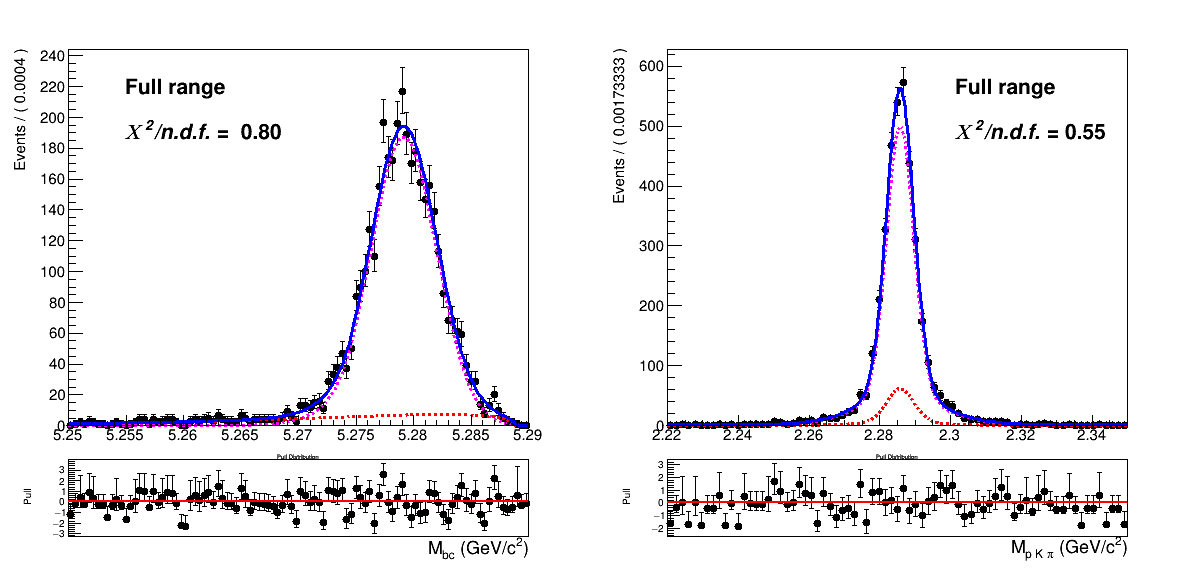
\includegraphics[width=0.75\textwidth]{06-chargedAnticorrBtoLambda/figs/stream12345_TotalSignal_charged_anticorrLambdaC_2Dfit.png}}
\caption{Two dimensional fit of total signal events in $M_{bc}$  and $M(p K \pi)$.}
\label{fig:stream12345_TotalSignal_charged_anticorrLambdaC_2Dfit}
\end{figure}

\begin{figure}[H]
\centering
{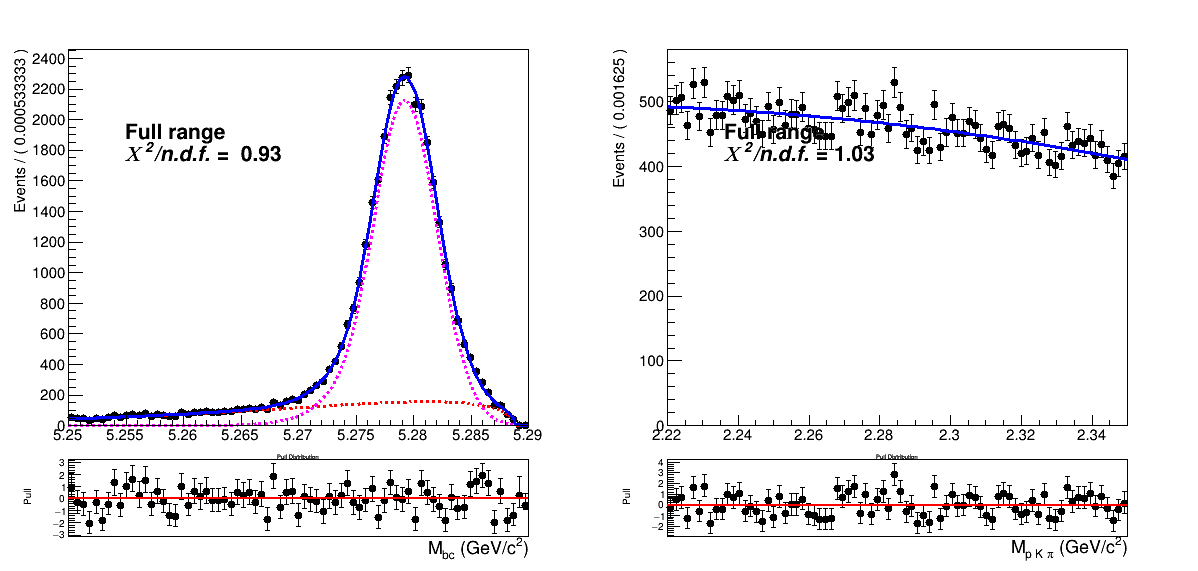
\includegraphics[width=0.75\textwidth]{06-chargedAnticorrBtoLambda/figs/streams12345_charged_anticorrLambdaC_Generic_2DFit.png}}
\caption{Two dimensional fit of generic ($B^+B^-$) events in $M_{bc}$  and $M(p K \pi)$.}
\label{fig:streams12345_charged_anticorrLambdaC_Generic_2DFit}
\end{figure}

The same can be said about the misreconstructed $B^0$ events (Fig. \ref{fig:stream12345_Crossfeed_charged_anticorrLambdaC_2Dfit})

\begin{figure}[H]
\centering
{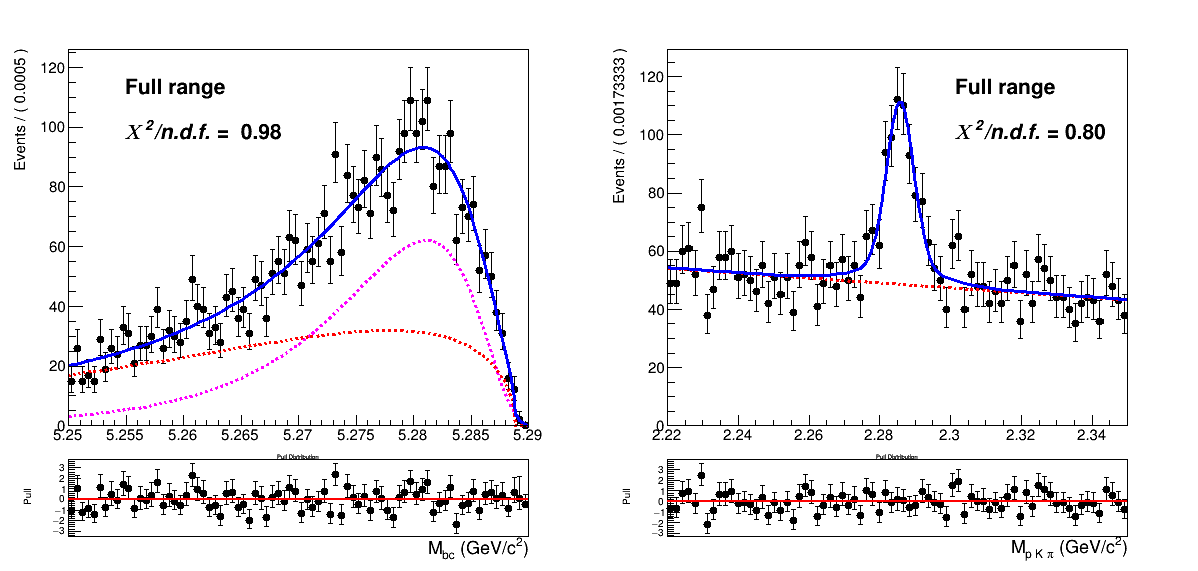
\includegraphics[width=0.75\textwidth]{06-chargedAnticorrBtoLambda/figs/stream12345_Crossfeed_charged_anticorrLambdaC_2Dfit.png}}
\caption{Two dimensional fit of crossfeed ($B^0\bar{B^0}$) events in $M_{bc}$  and $M(p K \pi)$.}
\label{fig:stream12345_Crossfeed_charged_anticorrLambdaC_2Dfit}
\end{figure}

\noindent To check that the shapes determined using 5 streams of Monte Carlo are describing with reasonable accuracy the 2D distribution, the projections of the fit of the two-dimensional distributions in the signal and sideband regions are plotted (\cref{fig:Signal_window_stream02345_Crossfeed_charged_anticorrLambdaC_2Dfit} - \cref{fig:InvM_Sideband_stream02345_Crossfeed_charged_anticorrLambdaC_2Dfit}).
One can see the same tendencies of undershooting/overshooting the $\Lambda_c$ invariant mass peak, as in the case of charged correlated decays  (Figures \ref{fig:5streams_Signal_window_Crossfeed_charged_corrLambdaC_2Dfit} - \ref{fig:5streams_Mbc_Sideband_Crossfeed_charged_corrLambdaC_2Dfit}).
But when examining the independent Monte Carlo stream distribution overlaid by the determined PDF in the very same regions (see Figures \ref{fig:Signal_window_stream1_Crossfeed_charged_anticorrLambdaC_2Dfit} -\ref{fig:Mbc_Sideband_stream1_Crossfeed_charged_anticorrLambdaC_2Dfit})
those effects are so much diminished, according to the statistics, that the effects are within statistical fluctuations and therefore negligible, contrary to the case of charged flavor-correlated decays.


\begin{figure}[H]
\centering
{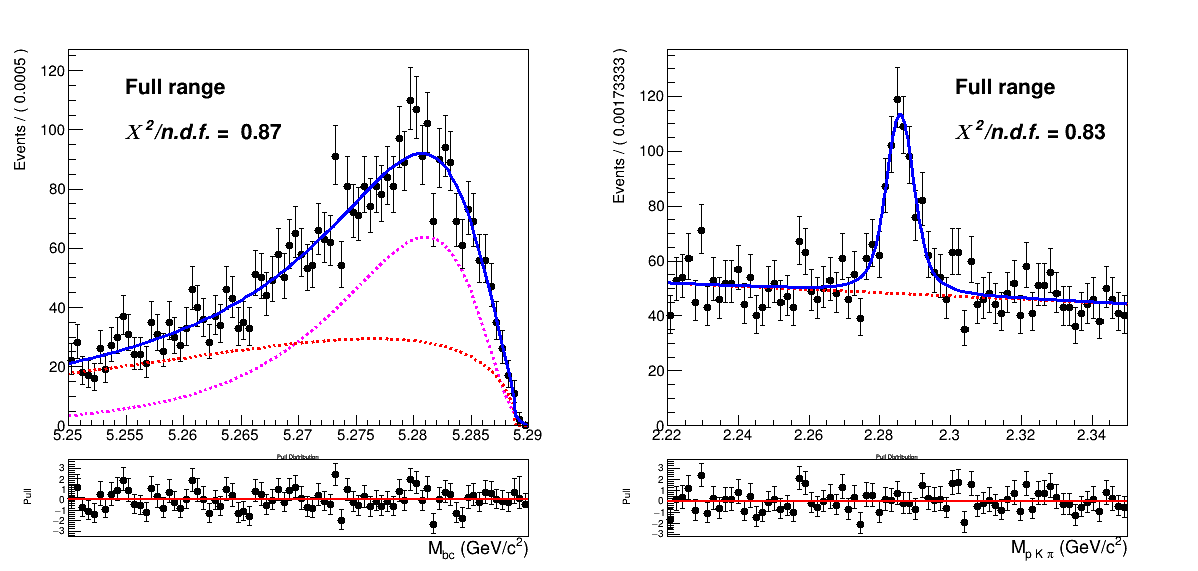
\includegraphics[width=0.75\textwidth]{06-chargedAnticorrBtoLambda/figs/stream02345_Crossfeed_charged_anticorrLambdaC_2Dfit.png}}
\caption{Two dimensional fit of crossfeed ($B^0\bar{B^0}$) events in $M_{bc}$  and $M(p K \pi)$.}
\label{fig:stream02345_Crossfeed_charged_anticorrLambdaC_2Dfit}
\end{figure}


\begin{figure}[H]
\centering
{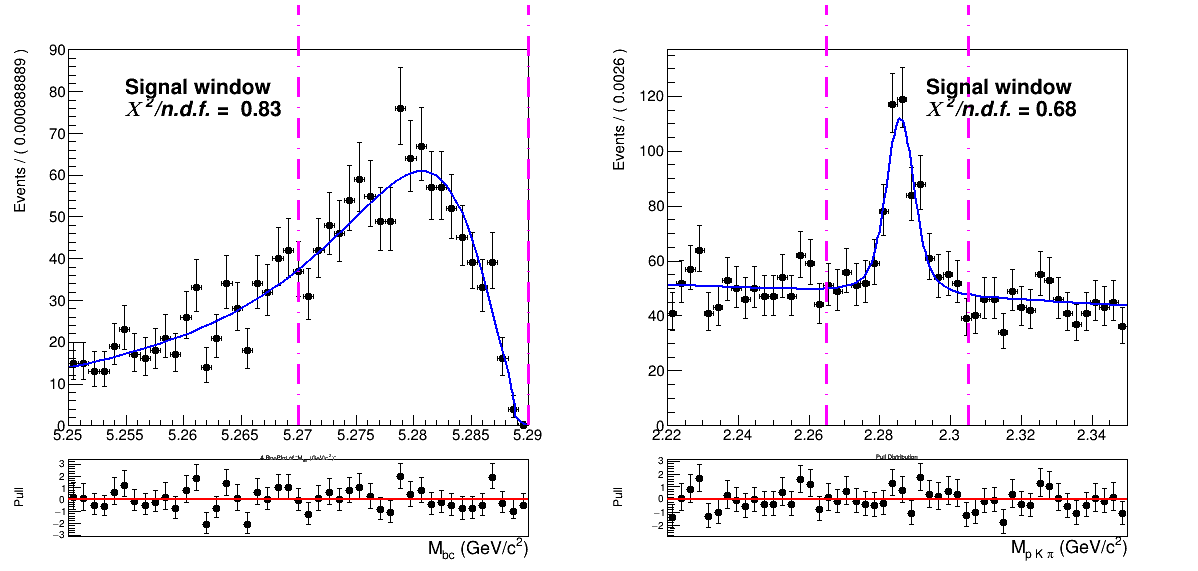
\includegraphics[width=0.75\textwidth]{06-chargedAnticorrBtoLambda/figs/Signal_window_stream02345_Crossfeed_charged_anticorrLambdaC_2Dfit.png}}
\caption{Signal region projections in $M_{bc}$ and $M(p K \pi)$  of the fit of crossfeed events.}
\label{fig:Signal_window_stream02345_Crossfeed_charged_anticorrLambdaC_2Dfit}
\end{figure}

\begin{figure}[H]
\centering
{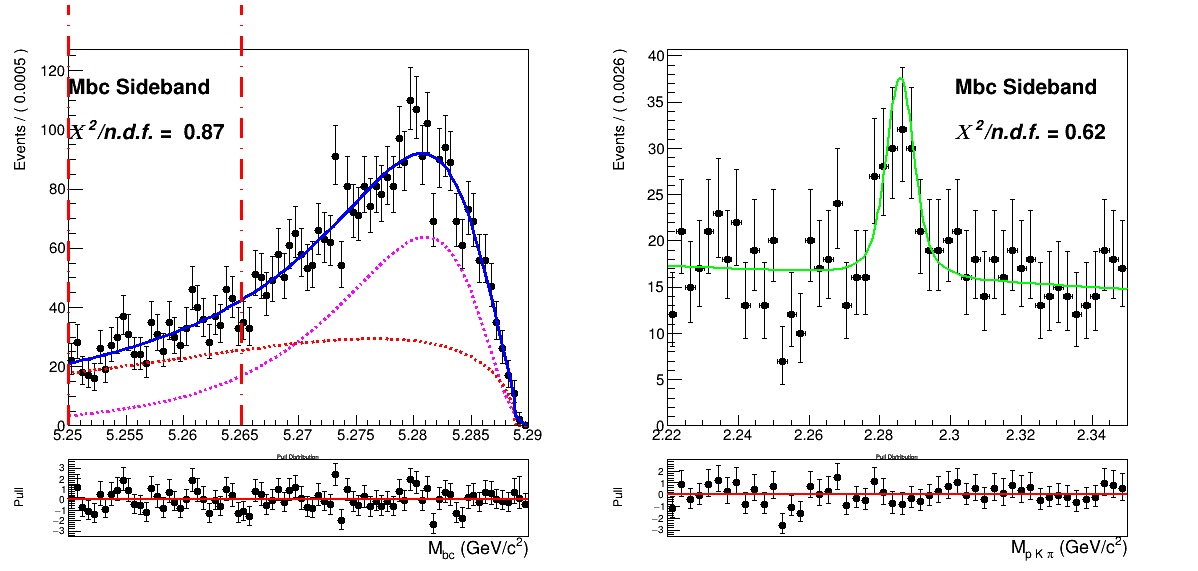
\includegraphics[width=0.75\textwidth]{06-chargedAnticorrBtoLambda/figs/Mbc_Sideband_stream02345_Crossfeed_charged_anticorrLambdaC_2Dfit.png}}
\caption{$M_{bc}$ sideband region projection of the fit of crossfeed events in $M(p K \pi)$.}
\label{fig:Mbc_Sideband_stream02345_Crossfeed_charged_anticorrLambdaC_2Dfit}
\end{figure}



\begin{figure}[H]
\centering
{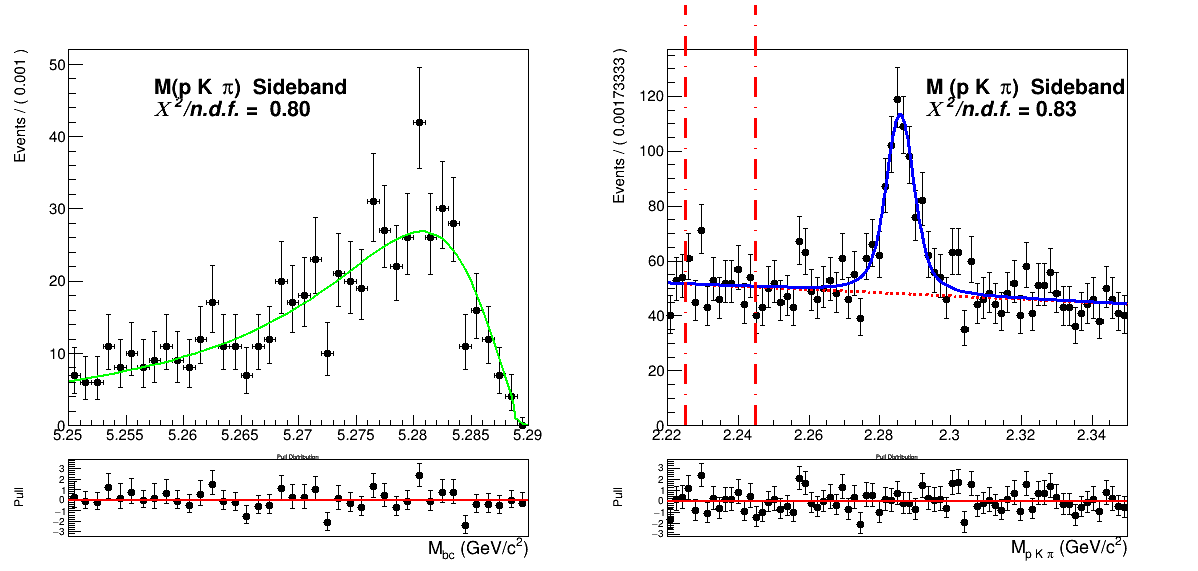
\includegraphics[width=0.75\textwidth]{06-chargedAnticorrBtoLambda/figs/InvM_Sideband_stream02345_Crossfeed_charged_anticorrLambdaC_2Dfit.png}}
\caption{$M(p K \pi)$ sideband region projection of the fit of crossfeed events in $M_{bc}$.}
\label{fig:InvM_Sideband_stream02345_Crossfeed_charged_anticorrLambdaC_2Dfit}
\end{figure}




\begin{figure}[H]
\centering
{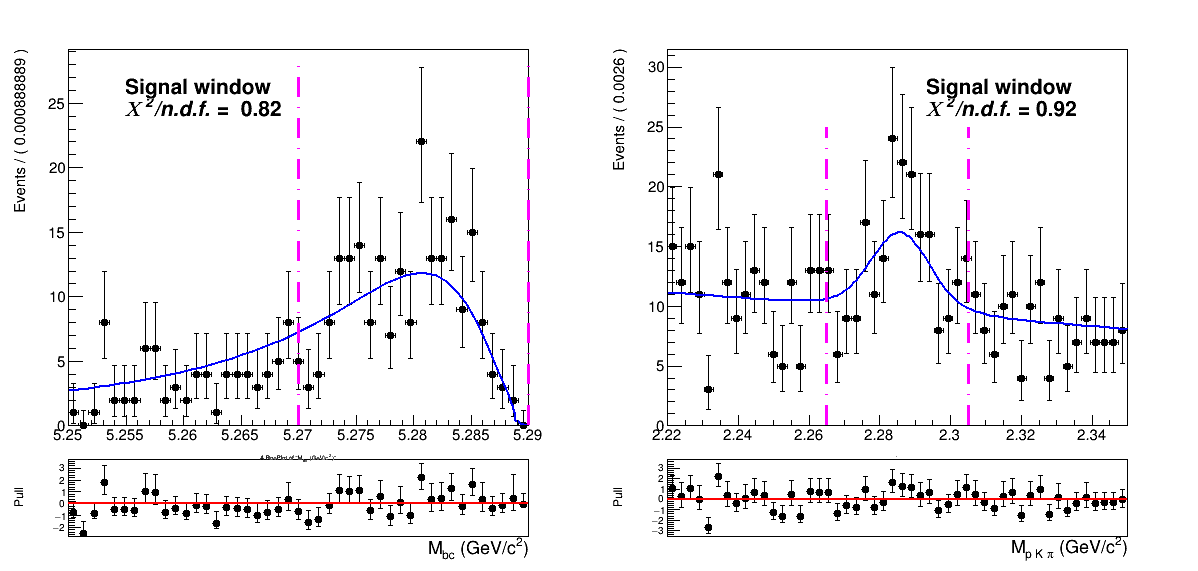
\includegraphics[width=0.75\textwidth]{06-chargedAnticorrBtoLambda/figs/Signal_window_stream1_Crossfeed_charged_anticorrLambdaC_2Dfit.png}}
\caption{Signal region projections in $M_{bc}$ and $M(p K \pi)$  of the fit of crossfeed events.}
\label{fig:Signal_window_stream1_Crossfeed_charged_anticorrLambdaC_2Dfit}
\end{figure}


\begin{figure}[H]
\centering
{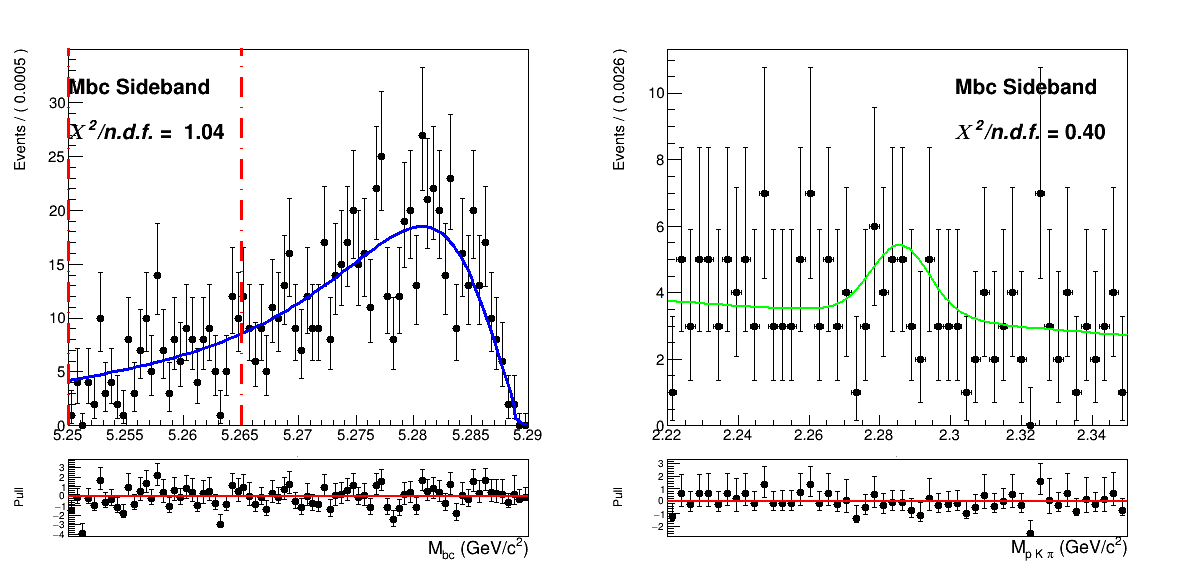
\includegraphics[width=0.75\textwidth]{06-chargedAnticorrBtoLambda/figs/Mbc_Sideband_stream1_Crossfeed_charged_anticorrLambdaC_2Dfit.png}}
\caption{Two dimensional fit of crossfeed ($B^0\bar{B^0}$) events in $M_{bc}$  and $M(p K \pi)$.}
\label{fig:Mbc_Sideband_stream1_Crossfeed_charged_anticorrLambdaC_2Dfit}
\end{figure}

\begin{figure}[H]
\centering
{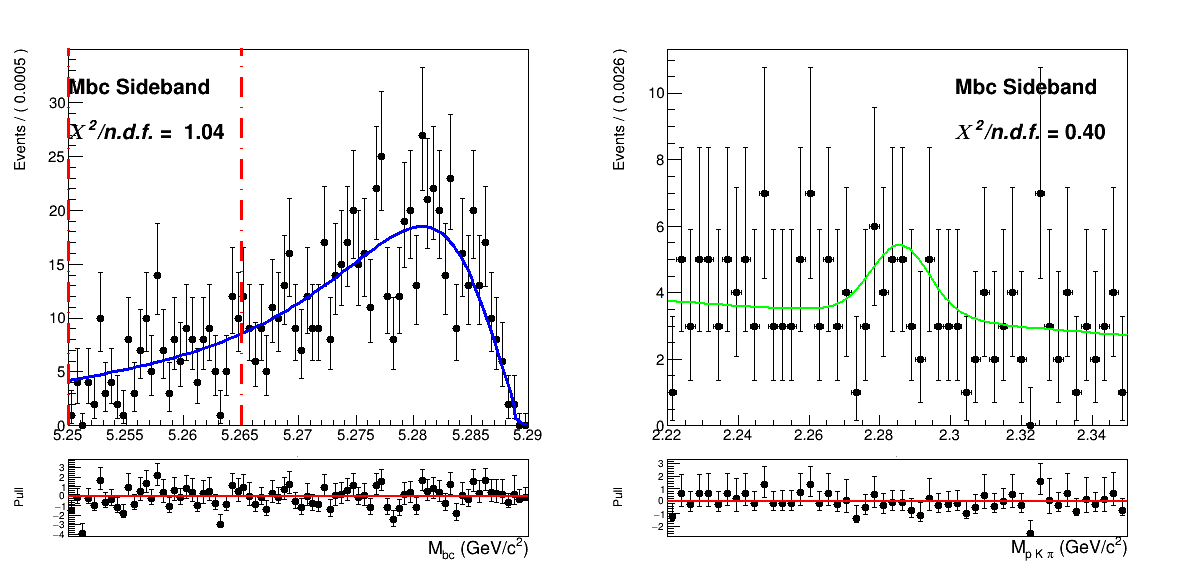
\includegraphics[width=0.75\textwidth]{06-chargedAnticorrBtoLambda/figs/Mbc_Sideband_stream1_Crossfeed_charged_anticorrLambdaC_2Dfit.png}}
\caption{Two dimensional fit of crossfeed ($B^0\bar{B^0}$) events in $M_{bc}$  and $M(p K \pi)$.}
\label{fig:Mbc_Sideband_stream1_Crossfeed_charged_anticorrLambdaC_2Dfit}
\end{figure}


\begin{figure}[H]
\centering
{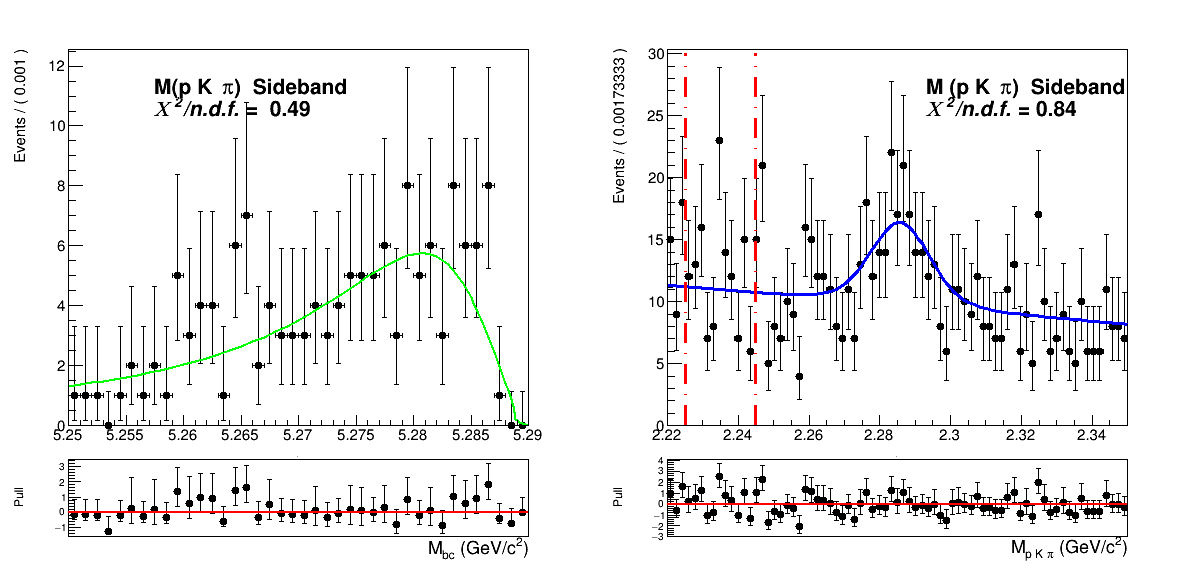
\includegraphics[width=0.75\textwidth]{06-chargedAnticorrBtoLambda/figs/InvM_Sideband_stream1_Crossfeed_charged_anticorrLambdaC_2Dfit.png}}
\caption{Two dimensional fit of crossfeed ($B^0\bar{B^0}$) events in $M_{bc}$  and $M(p K \pi)$.}
\label{fig:InvM_Sideband_stream1_Crossfeed_charged_anticorrLambdaC_2Dfit}
\end{figure}


\vspace{2.5 cm}

\noindent  The procedure adopted to model the continuum background is the same used for the charged correlated $B \rightarrow \Lambda_c$ decays. To obtain the shape that can describe the continuum background  $M_{bc}$ distribution, the continuum suppression is not applied on the off-resonance continuum sample in order to acquire more statistics. It is then scaled and corrected for the \textit{SignalProbability} correlated effects. The scaling and bin-correction procedure was carried out on a sample of five streams of on- and off-resonance MC. From a ratio plot, like the one in Fig. \ref{fig:stream02345_charged_anticorrLambdaC_woCScuts_Mbc_scaling}, showing the continuum on-resonance distribution in $M_{bc}$ and the scaled continuum on-resonance distribution without the continuum suppression applied, the bin-correction is obtained to correct the off-resonance data in the scaling procedure. The validity of this procedure is first tested on the sixth independent MC sample:      
Fig. \ref{fig:MC_on_off_resonance_stream2_anticorrLambda_continuum_2D_Mbc_corrected} shows the scaled and bin-corrected off-resonance continuum histogram compared with the continuum on-resonance distribution of the independent stream. 
Compared to the charged correlated decays one can notice larger statistical fluctuations but the overall result looks still fairly reasonable. In order to obtain the PDF describing the distribution the histogram is fitted (see Fig. \ref{fig:stream2_rescaledMbc_40binsHist_Novosibirsk}), i.e. with a Novosibirsk function. \\
Since in the $\Lambda_c$ invariant mass one doesn't expect correlation effects, one can fit directly the properly scaled distribution with a first order polynomial (see Fig.\ref{fig:stream02345_anticorrLambdaC_total_continuum_InvM_Fit_off})
\noindent It is possible then to check the validity of the whole procedure on the on-resonance Monte Carlo independent stream (Fig. \ref{fig:stream1_anticorrLambddaC_total_continuum_2DFit_Novosibirsk})  


\begin{figure}[H]
\centering
\subcaptionbox{\label{fig:stream02345_charged_anticorrLambdaC_woCScuts_Mbc_scaling}}
{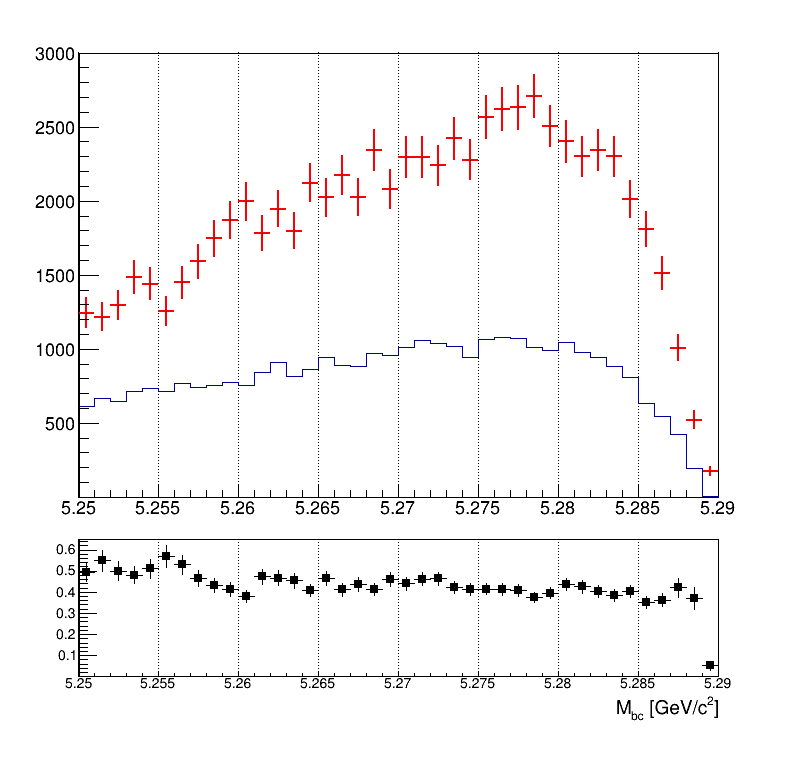
\includegraphics[width=.45\textwidth]{06-chargedAnticorrBtoLambda/figs/stream02345_charged_anticorrLambdaC_woCScuts_Mbc_scaling.png}} \quad
\subcaptionbox{\label{fig:MC_on_off_resonance_stream2_anticorrLambda_continuum_2D_Mbc_corrected}}
{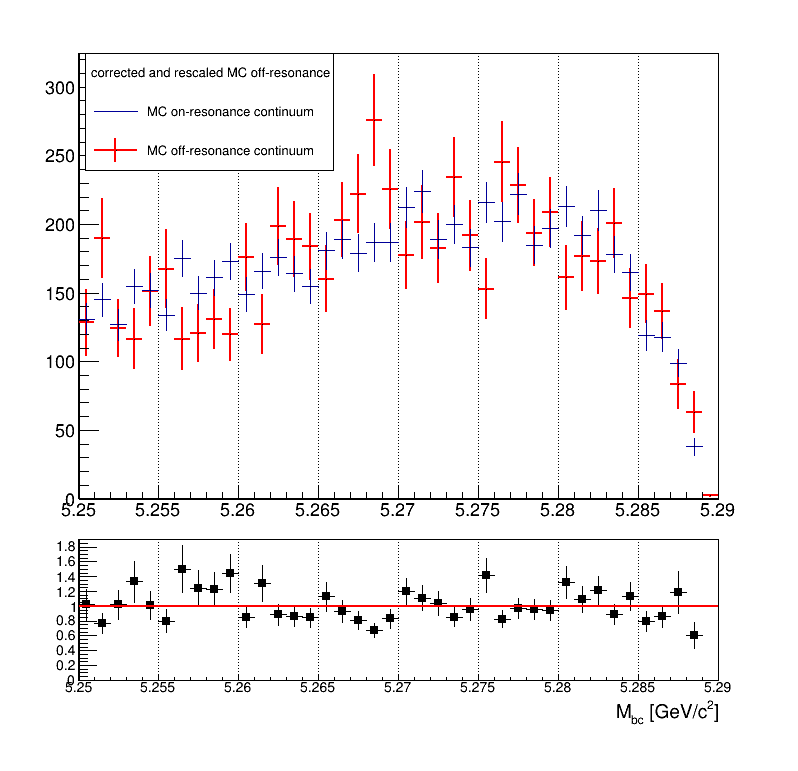
\includegraphics[width=.45\textwidth]{06-chargedAnticorrBtoLambda/figs/MC_on_off_resonance_stream2_anticorrLambda_continuum_2D_Mbc_corrected.png}} \quad
\caption{On the left: $M_{bc}$ distributions of the MC off-resonance sample without continuum suppression and the MC continuum sample with applied continuum suppression (5 streams). On the right: $M_{bc}$ distributions of the corrected scaled MC off-resonance and on-resonance MC continuum (independent stream).}
\end{figure}


\begin{figure}[H]
\centering
\subcaptionbox{\label{fig:stream2_rescaledMbc_40binsHist_Novosibirsk}}
{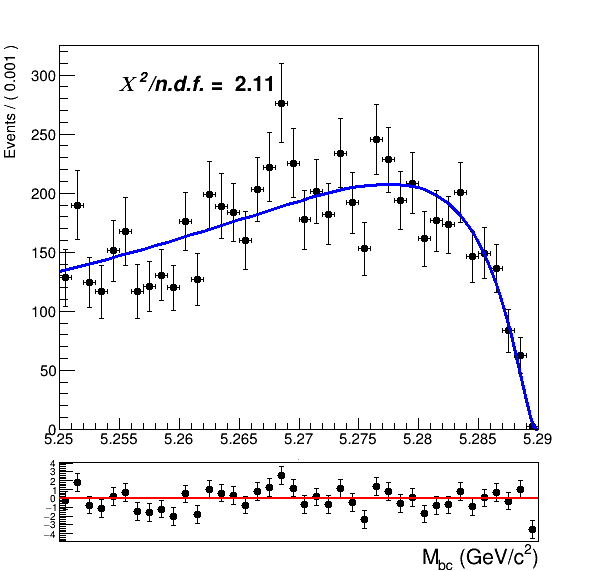
\includegraphics[width=0.45\textwidth]{06-chargedAnticorrBtoLambda/figs/stream2_rescaledMbc_40binsHist_Novosibirsk.png}} \quad
\subcaptionbox{\label{fig:stream02345_anticorrLambdaC_total_continuum_InvM_Fit_off}}
{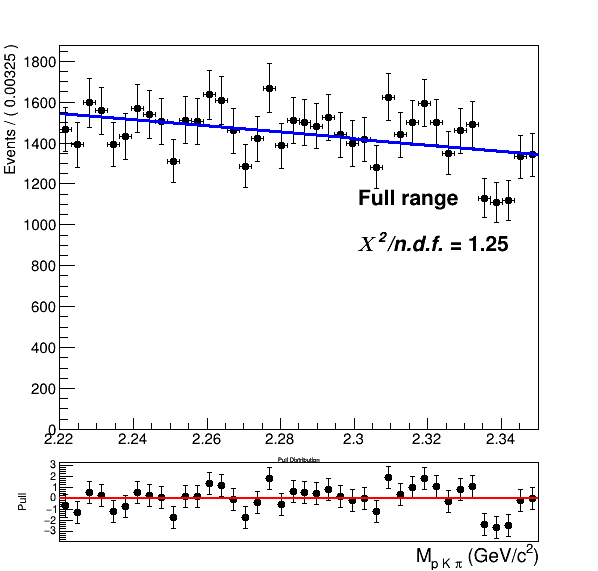
\includegraphics[width=.45\textwidth]{06-chargedAnticorrBtoLambda/figs/stream02345_anticorrLambdaC_total_continuum_InvM_Fit_off-resonance.png}} \quad
\caption{On the left: fit of the $M_{bc}$ distribution MC (scaled and corrected) off-resonance continuum (one stream). On the right: fit of the $\Lambda_c$ invariant mass distribution of five stream scaled off-resonance continuum.}
%\label{fig:stream2_rescaledMbc_40binsHist_Novosibirsk}
\end{figure}


\begin{figure}[H]
\centering
{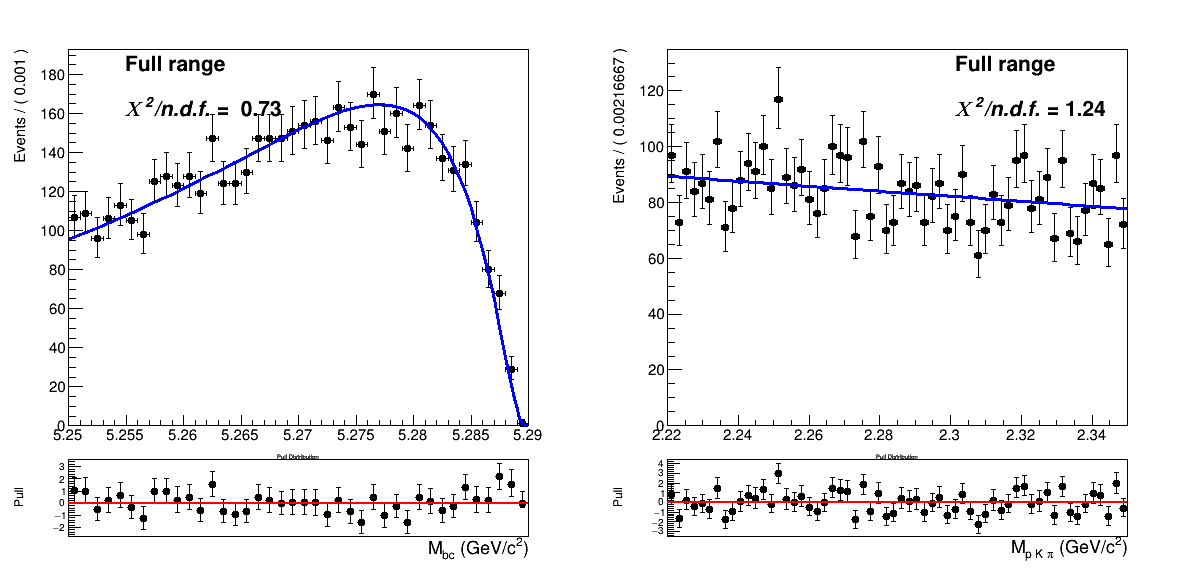
\includegraphics[width=0.85\textwidth]{06-chargedAnticorrBtoLambda/figs/stream1_anticorrLambddaC_total_continuum_2DFit_Novosibirsk.png}}
\caption{Continuum $M_{bc}$  and $M(p K \pi)$ distributions overlaid by the PDFs obtained in fits shown in Figures \ref{fig:stream2_rescaledMbc_40binsHist_Novosibirsk} - \ref{fig:stream02345_anticorrLambdaC_total_continuum_InvM_Fit_off}}
\label{fig:stream1_anticorrLambddaC_total_continuum_2DFit_Novosibirsk}
\end{figure}

\subsection{Two dimensional fit}\label{sec:chargedAnticorr2DtotalFit}
After obtaining the PDFs describing the various signal/background components using five streams statistics, the fit model is tested with six fits on the six independent Monte Carlo streams. The conditions for these six two dimensional fits are again the same used for the charged correlated decays (see Sec. \ref{2DtotalFit}).
\noindent Exemplary, the distributions of stream 0 overlaid by the fitted PDF are depicted in Fig. \ref{fig:Total_2DFit_stream0_chargedAnticorrLambdaC_Crossfeed_fraction} (see \cref{sec:chargedAnticorrApp}                       
for the projections in signal and sideband regions). 
In Table \ref{tab:SixStreams_chargedCorrLam2Dfits} the signal yields of the fits (\textbf{Reconstructed Signal}) to the two dimensional distributions for the six streams of $B^- \rightarrow \bar{\Lambda_c}^-$ flavor-anticorrelated decays are listed and compared to the expected yields of reconstructed signal, and fitted and truth-matched total signal events are also compared, together with their deviations.

\begin{figure}[H]
\centering
{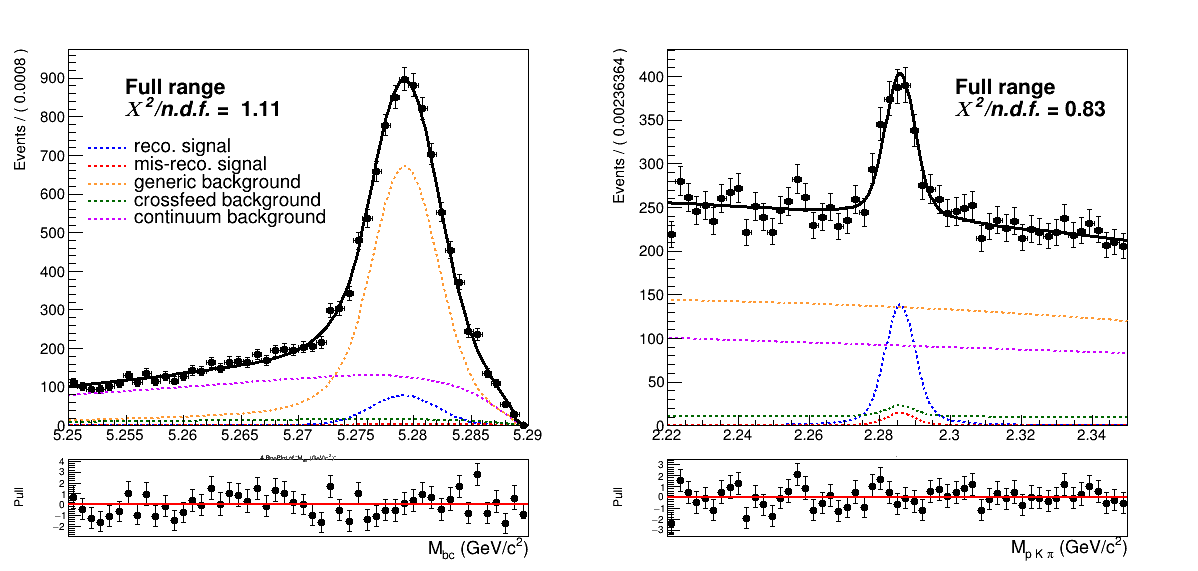
\includegraphics[width=0.85\textwidth]{06-chargedAnticorrBtoLambda/figs/Total_2DFit_stream0_chargedAnticorrLambdaC_Crossfeed_fraction_parametrization.png}}
\caption{Two dimensional fit on stream 0 Monte Carlo simulated data.}
\label{fig:Total_2DFit_stream0_chargedAnticorrLambdaC_Crossfeed_fraction}
\end{figure}

\begin{table}[h]
\centering
\resizebox{0.8\textwidth}{!}{%
\setlength{\tabcolsep}{8pt}
\begin{tabular}{c c c c c c c}

\toprule
 \hline
   &	\multicolumn{2}{c}{Reconstructed Signal}  & \multicolumn{2}{c}{Total Signal} &  \\
     &  fit \hspace{0.5 cm}  & expected  & fit   & MC truth &  \multicolumn{2}{c}{fit - MC truth} \\
 \midrule
 \hline
stream 0	&	730 $\pm$ 60 	&	660 $\pm$ 21	&	805 $\pm$ 65	&	765	&  40	&	5.2 $\%$	\\
stream 1	&	732 $\pm$ 60	&	698 $\pm$ 29	&	794 $\pm$ 63	&	785	&  9	&	1.1$\%$	\\
stream 2	&	759 $\pm$ 65	&	718 $\pm$ 29	&	800 $\pm$ 67	&	797	& 3	&	0.4$\%$	\\
stream 3	&	725 $\pm$ 58	&	702 $\pm$ 29	&	769 $\pm$ 60	&	802	& -33	&	-4.1$\%$	\\
stream 4	&	829 $\pm$ 67	&	710 $\pm$ 29	&	944 $\pm$ 76	&	804	& 140  	&	17.4$\%$	\\
stream 5	&	650 $\pm$ 61	&	675 $\pm$ 29	&	703 $\pm$ 62	&	760	&  -57	&	-8.1$\%$	\\
\midrule
\hline
sum			&	4425		&	4163	&		4815		&	4718	&	102	&	+ 2.2$\%$	\\
\bottomrule
\hline
\end{tabular}%
}%
\caption{Comparison of fitted and expected signal yields, fitted and truth-matched total signal for six streams of Belle generic MC when fitting the two dimensional distributions of $M_{bc}$ and $M(p K \pi)$.}
\label{tab:SixStreams_chargedAnticorrLam2Dfits}
\end{table}

\noindent Except for stream 4 all the fits show values of reconstructed signal within the 1$\sigma$ uncertainties in agreement with the expected ones, 
but as already encountered in Sec. \ref{2DtotalFit} a tendency of overestimation can be seen also in these fits, confirmed by the fit shown in Fig \ref{fig:RecoSignal_streams_fittedPoints_charged_anticorrLambdaC}. Again this small, but not negligible, bias has to  be taken into account while fitting the data.


\begin{figure}[H]
\centering
{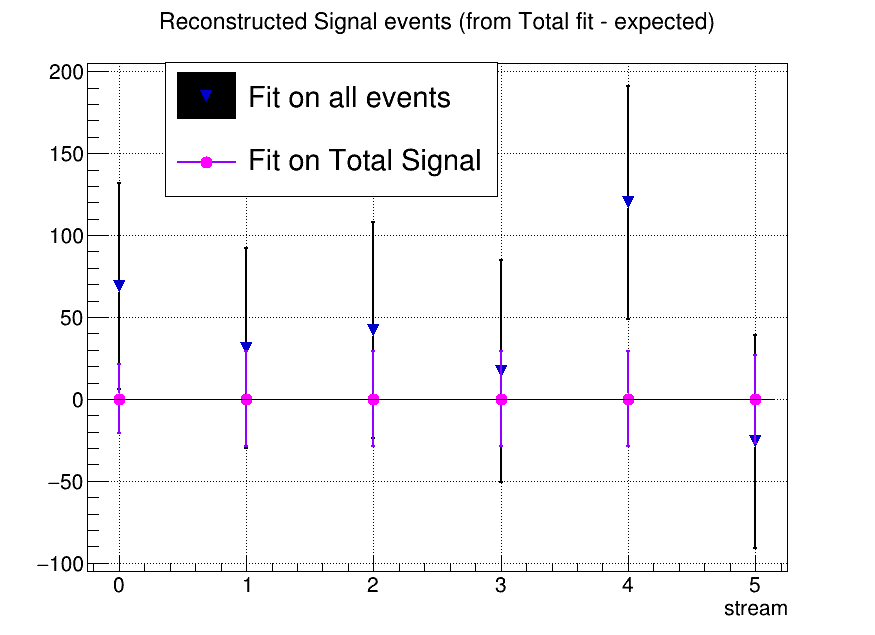
\includegraphics[width=0.75\textwidth]{06-chargedAnticorrBtoLambda/figs/Fitted_RecoSignal_chargedAntiCorrLambdaC.png}}
\caption{Differences between results from the fits and "expected" values for signal yields as reported in the first columns on Table \ref{tab:SixStreams_chargedAnticorrLam2Dfits} .}
\label{fig:chargedAnticorrRecoSignal_fit-expectedPlot}
\end{figure}

\begin{figure}[H]
\centering
{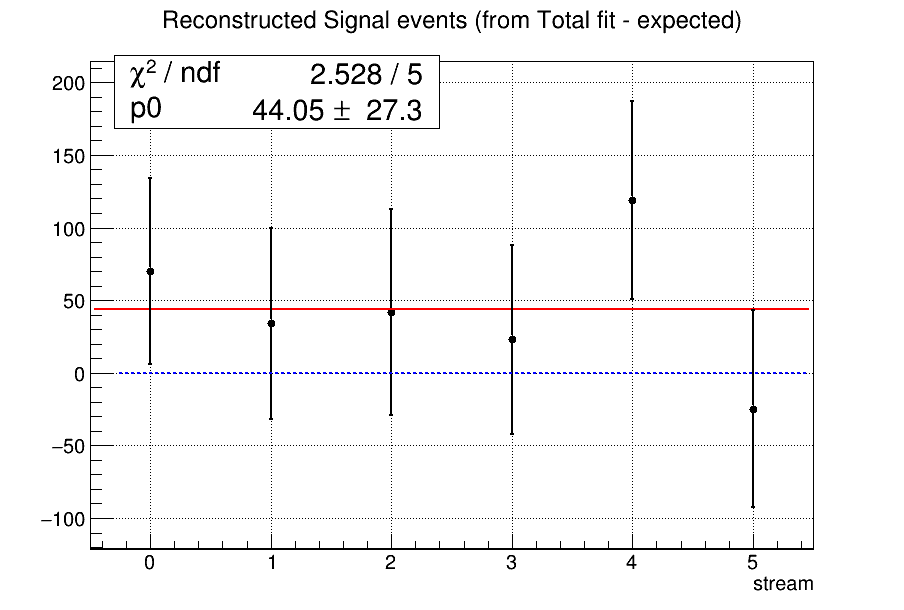
\includegraphics[width=0.85\textwidth]{06-chargedAnticorrBtoLambda/figs/RecoSignal_streams_fittedPoints_chargedAnticorrLambdaC_w_CrossfeedRatio_param.png}}
\caption{}
\label{fig:RecoSignal_streams_fittedPoints_charged_anticorrLambdaC}
\end{figure}

\noindent  Also the behaviour for different signal-to-background ratio was investigated using the six independent streams of continuum and all the ten independent streams of $B\bar{B}$ events for the generic and crossfeed backgrounds and for the signal events. 
The amount of total signal is varied between 50$\%$ and 275$\%$ of the nominal (MC) values, in order to cover the values spanned by the uncertainties on the measurement perfromed by $BaBar$ ($\mathcal{B}(B^+ \rightarrow \bar{\Lambda}_c^+ X) = 2.1^{+0.9}_{-0.6} $)
 and even the values covered by twice larger uncertainties as one can see in \cref{fig:Charged_anticorrLambda_BR_LinearityTest}. 
The values seem to distribute according to a linear dependence,  therefore also for this decay channel one doesn't expect any systematics due to different signal-to-background ratio.% The linear fit suggests a compatibility with a 1:1 relation: the red and the blue dotted lines don't overlap, but the values of the fitted line are compatible within the uncertainties with the identity line. Though also in this second test we see a slight tendency of overshooting the expected values.   


\begin{figure}[H]
%\centering
{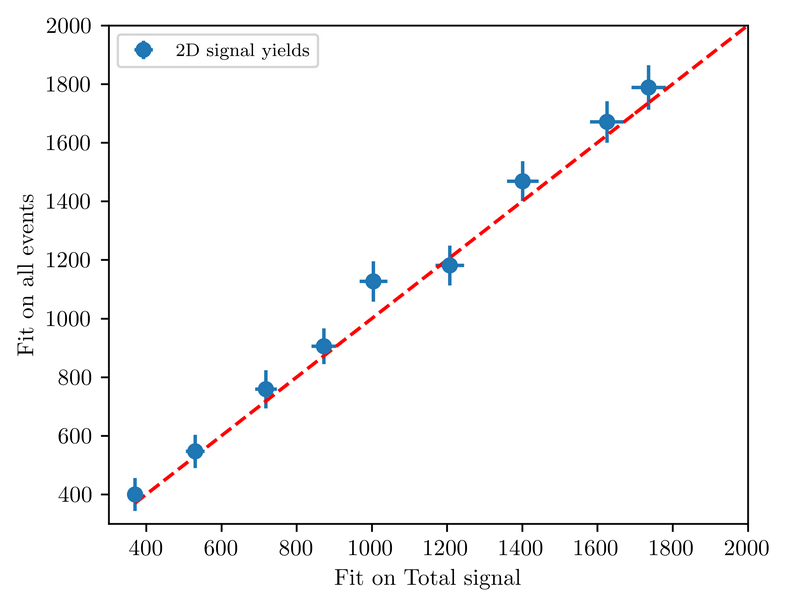
\includegraphics[width=0.75\textwidth]{06-chargedAnticorrBtoLambda/figs/Charged_anticorrLambda_LinearityTest.png}}
\caption{Linearity test: on the x-axis the obtained reconstructed signal yields from fits on different amounts of total signal; on y-axis the yields of reconstructed signal obtained fitting all events
 (as in Fig. \ref{fig:stream0_Total2Dfit_charged_corrLambdaC}). The dashed red line represents the 1:1 linear dependence.}
\label{fig:Charged_anticorrLambda_LinearityTest}
\end{figure}



\begin{figure}[H]  
  %\centering
{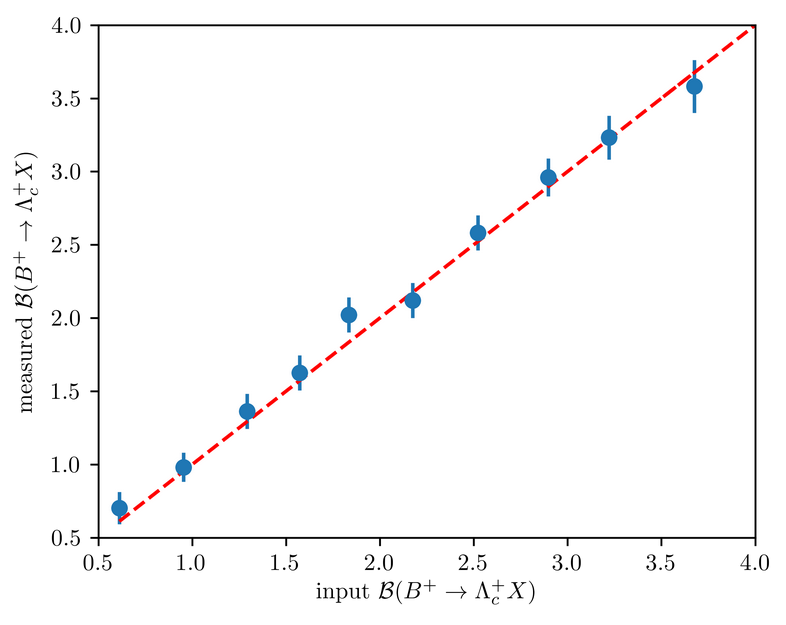
\includegraphics[width=0.75\textwidth]{06-chargedAnticorrBtoLambda/figs/Charged_anticorrLambda_BR_LinearityTest.png}}
\caption{Linearity test: on the x-axis the input branching ratio value corresponding to the signal yields displayed on the x-axis in \cref{fig:Charged_anticorrLambda_LinearityTest}; 
on y-axis the measured branching fraction values corresponding to the signal yields of reconstructed signal displayed on the y-axis in \cref{fig:Charged_anticorrLambda_LinearityTest}.}
\label{fig:Charged_anticorrLambda_BR_LinearityTest}
\end{figure}

\noindent  Toy MC pseudo-experiments were performed as well (see Appendix).%, which also don't show evidence of any bias on the signal yields. 
 
\newpage

\subsection{Probability Density Functions (PDFs) for the $B_{tag}$}
The $M_{bc}$ distribution of the tagged  $B$ mesons is fitted with a Crystal Ball as for the "peaking" component and the "flat" component is fitted with a Argus function (Fig. \ref{fig:stream0_anticorr_chargedBtag_Total_Signal_fit}).
The crossfeed background, consisting of neutral $B$ mesons tagged as charged $B$, is fitted instead with a sum of a Novosibirsk and an asymmetric Gaussian PDF (Fig. \ref{fig:NeutralCrossfeed_stream0_anticorrLambdaC_chargedBtag_MbcFit}).


\begin{figure}[H]
\begin{minipage}{.5\textwidth}
\centering
\subcaptionbox{\label{fig:stream0_anticorr_chargedBtag_Total_Signal_fit}}
{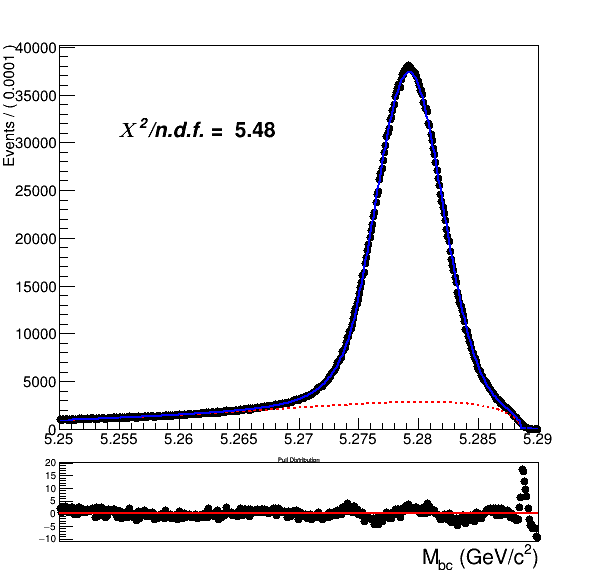
\includegraphics[width=0.80\textwidth]{06-chargedAnticorrBtoLambda/figs/stream0_anticorr_chargedBtag_Total_Signal_fit.png}}
\end{minipage} 
 \begin{minipage}{.5\textwidth}
\subcaptionbox{\label{fig:NeutralCrossfeed_stream0_anticorrLambdaC_chargedBtag_MbcFit}}
{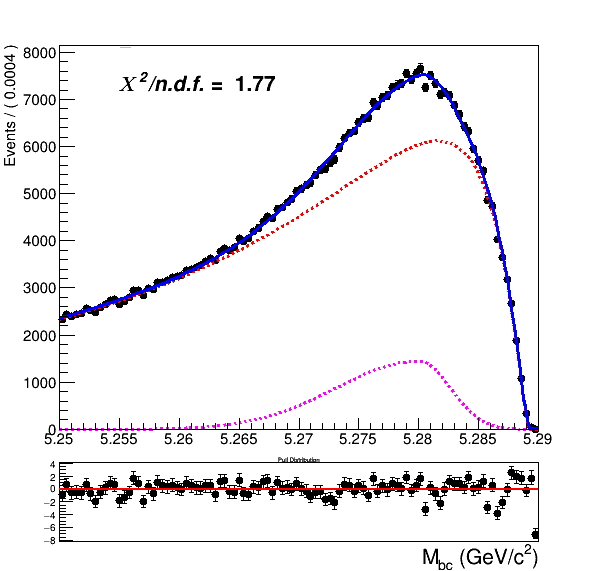
\includegraphics[width=0.80\textwidth]{06-chargedAnticorrBtoLambda/figs/NeutralCrossfeed_stream0_anticorrLambdaC_chargedBtag_MbcFit.png}}
\end{minipage}
\caption{On the left: fitted distribution of tagged charged $B$ mesons, reconstructed signal events (magenta) are described by a Crystal Ball whereas the misreconstructed signal events (red) are described by an Argus function. On the right: Crossfeed distribution fitted with a sum of Novosibirsk (red) and asymmetric Gaussian PDF (magenta)}
\end{figure}


\vspace{0.25 cm}

\noindent As for the continuum background, same procedure as the one in the case of charged flavor-correlated decays is adopted:

\begin{itemize}
    \item first the off-resonance sample is scaled accordingly with all the included cuts.
    \item the ratio between the scaled off-resonance and the on-resonance in MC is calculated in each bin (see Fig. \ref{fig:stream0_chargedAnticorrBtag_off-on_resonance})
    \item the bin-correction is applied on an independent stream and the scaled and bin-corrected $M_{bc}$ distribution is compared with the on-resonance distribution as shown in Fig. \ref{fig:stream1_chargedB_anticorrLambdaCoffresonance_scaled_check}
\end{itemize}

\begin{figure}[H]
 \centering
\subcaptionbox{\label{fig:stream0_chargedAnticorrBtag_off-on_resonance}}
{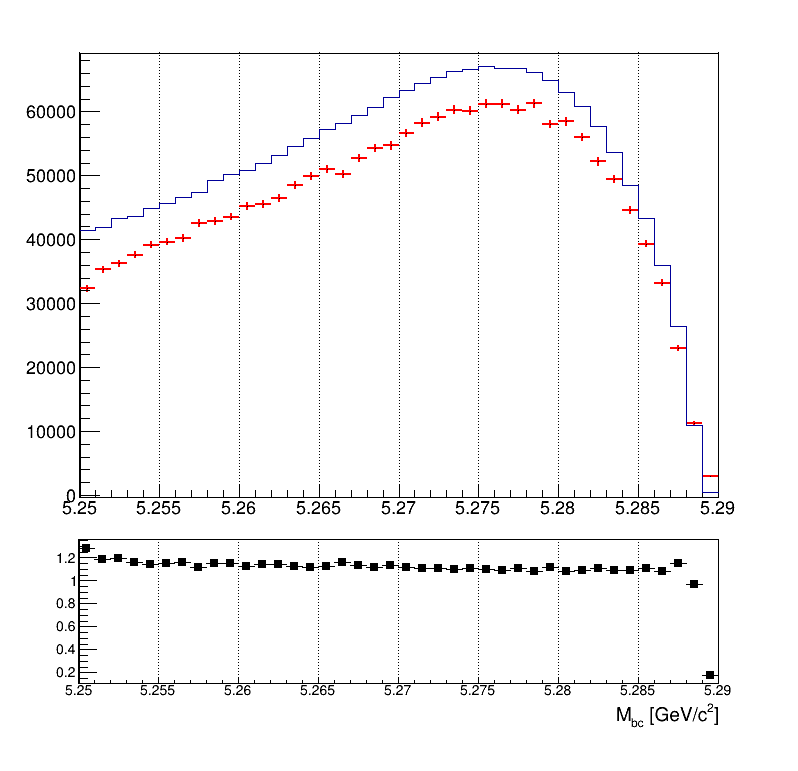
\includegraphics[width=.45\textwidth]{06-chargedAnticorrBtoLambda/figs/on_scaled_offRes_stream0_continuum.png}}
\subcaptionbox{\label{fig:stream1_chargedB_anticorrLambdaCoffresonance_scaled_check}}
{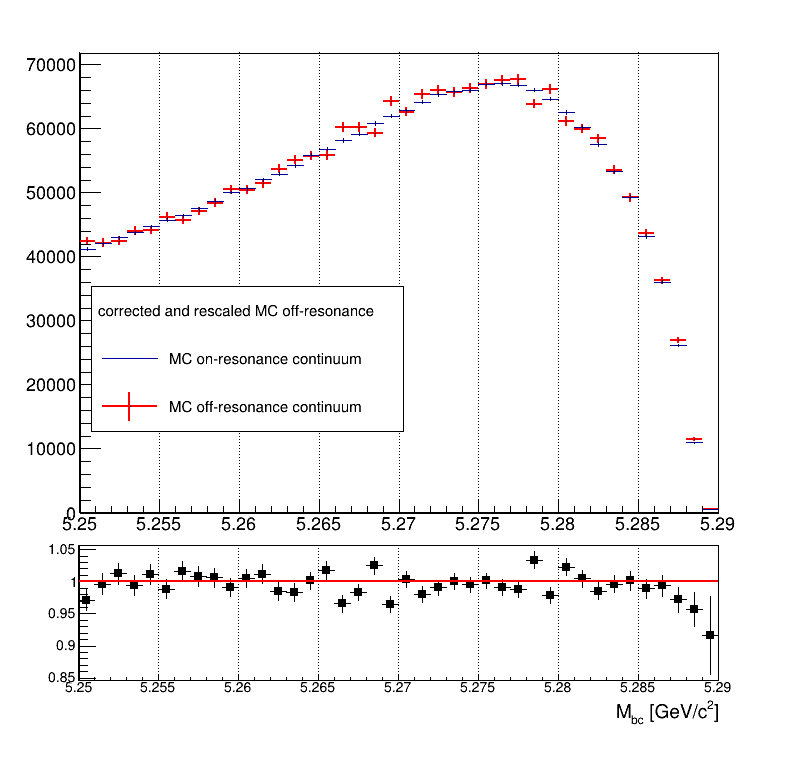
\includegraphics[width=.44\textwidth]{06-chargedAnticorrBtoLambda/figs/stream1_chargedB_anticorrLambdaCoffresonance_scaled_check.png}} 
\caption{On the left: $M_{bc}$ distributions of the MC off-resonance sample and the MC continuum sample with applied continuum suppression. On the right: $M_{bc}$ distributions of the corrected scaled MC off-resonance and on-resonance MC continuum.}
\end{figure}


\newpage
\subsection{ $B_{tag}$ fit}\label{sec:chargedAnticorrBtagFit}


\begin{figure}[h!]
\centering
{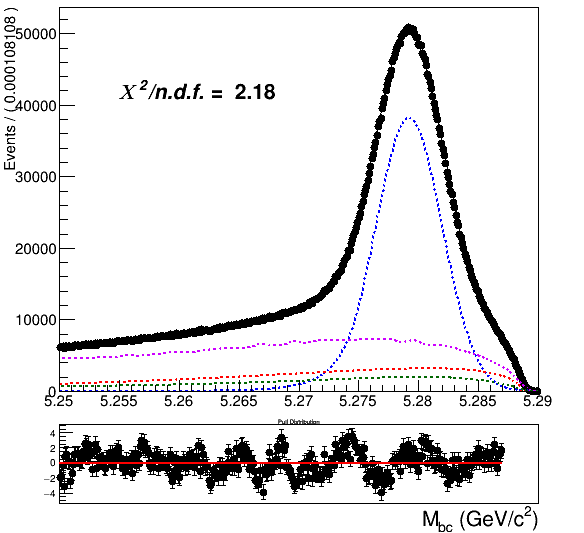
\includegraphics[width=0.50\textwidth]{06-chargedAnticorrBtoLambda/figs/stream1_chargedBtag_Total_fit_sigmaCB_misRecoSlope_free_370bins.png}}
\caption{Total fit of tagged $B$ mesons on Monte Carlo simulated data.}
\label{fig:chargedAnticorrLambdaC_BtagFit}
\end{figure}
\vspace{1.5cm} 

An independent Monte Carlo stream was used to test the total fit model on tagged $B$ meson candidates.
As in the 2D fit, the parameter for the width, $\sigma_{CB}$, of the Crystal Ball is floated and the ratio between expected crossfeed background events and  misreconstructed signal events is fixed from the MC. 
The Argus function describing the misreconstructed signal is also not fully constrained: the parameter describing the tail is free.
As in the previous $B_{tag}$ fits, the range for the fit is restricted to values betweeen 5.250 and 5.287 GeV/c$^2$.
Yields for the reconstructed and misreconstructed signal are obtained from the fit:\\
\vspace{0.25 cm}

\begin{tabular}{ |p{2.5cm}||p{4.2cm}|  }
 \hline
 NrecSig  & 2.5099$\cdot$10$^6 \pm$ 4408\\
 NmisSig &  7.82307$\cdot$10$^5 \pm$ 2936 \\
 \hline
\end{tabular}


\vspace{0.5 cm}
\noindent The Total Signal (the sum  NrecSig+NmisSig) is 3292168 $\pm$ 2423 (to be compared with 3299629 from the Monte Carlo), which means a $\sim 3\sigma$ underestimation. As in the case of charged flavor-correlated decays, this can produce some systematic effect which needs to be taken into account.
In fact, a slight underestimation of the Total Signal is found also in the result of the toy Monte Carlo study\footnote{as usual performed with  $3\times10^3$ pseudo-datasets}: \cref{fig:Total_Signal_chargedBtagToyMCstudy} shows the results for the Total Signal events and one can notice a mean value for the pulls consistently below zero.



\begin{figure}[H]
\centering
{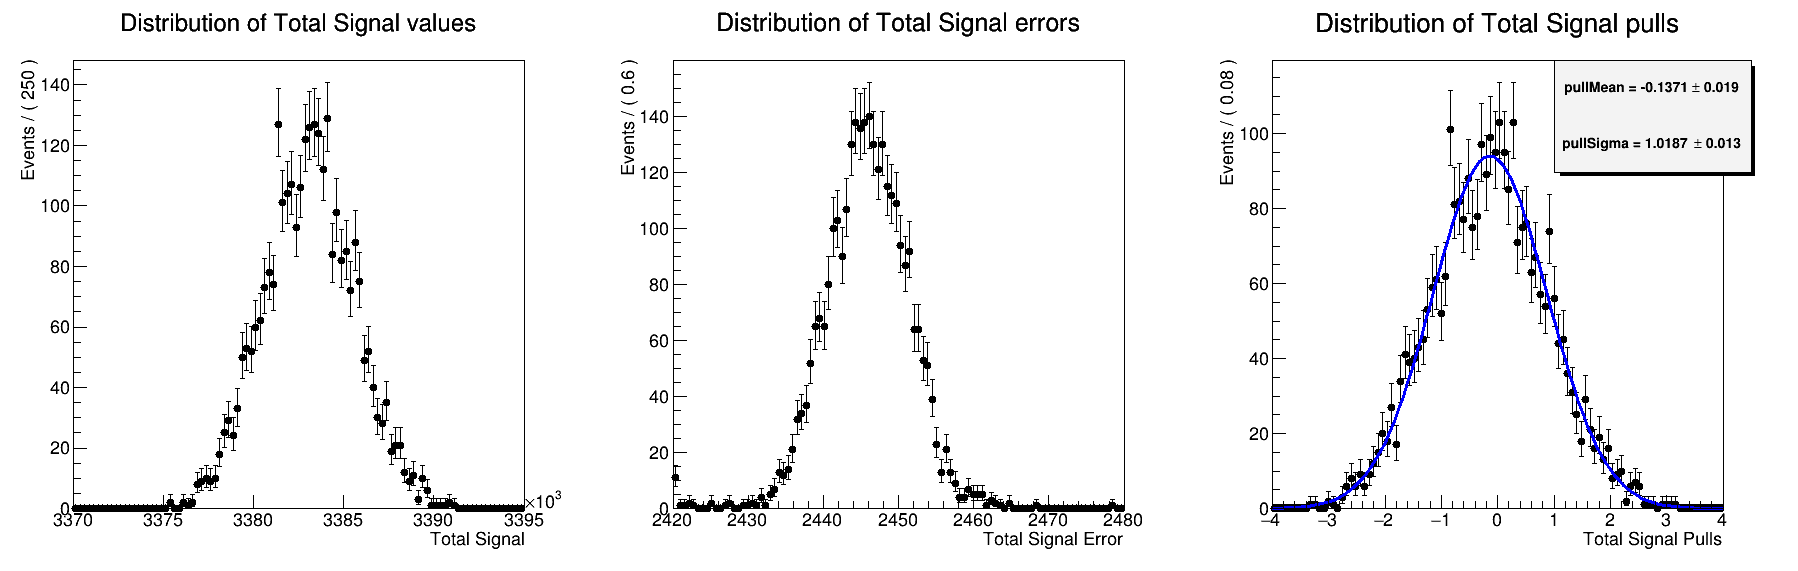
\includegraphics[width=1.\textwidth]{06-chargedAnticorrBtoLambda/figs/Total_Signal_chargedBtagToyMCstudy.png}}
\caption{Toy MC fits of pseudo-data showing the Total Signal yield (left), Total Signal yield errors (center) and the pull distribution of the Total Signal (right).}
\label{fig:Total_Signal_chargedBtagToyMCstudy}
\end{figure}


\subsection{$\Lambda_c$ and FEI efficiency}

The efficiency in reconstructing the ${\Lambda_c}$ baryon after correctly tagging the charged $B$ meson, is as usual estimated as the ratio: 

\begin{equation}
    \frac{N_{recSig}(B_{tag}, \Lambda_c)}{N_{recSig}(B_{tag}^{sig})}
\end{equation}

\vspace{0.5cm}

\noindent where $N_{recSig}(B_{tag}, \Lambda_c))$ are the yields of reconstructed signal from the two dimensional fits (reported in Table \ref{tab:SixStreams_chargedAnticorrLam2Dfits} ) and  $N_{recSig}(B_{tag}^{sig})$ are the yields of correctly reconstructed signal in a fit of $B$ mesons tagged in events where one of the two mesons decayed hadronically and inclusively into a ${\Lambda_c}$ baryon (see Fig \ref{fig:sixstreams_chargedBtagSignal_fit}). This ratio was calculated upon six streams of Monte Carlo simulated data.

\begin{figure}[h!]
\centering
{\includegraphics[width=0.40\textwidth]{06-chargedAnticorrBtoLambda/figs/chargedBtag_anticorrLambdaC_TotalSignalBtag_fit.png}}
\caption{Fit of tagged $B$ mesons in the "signal events" sample}
\label{fig:chargedBtag_anticorrLambdaC_TotalSignalBtag_fit}
\end{figure}


\vspace{0.5 cm}
From this and the results listed in \cref{sec:chargedAnticorr2DtotalFit} 
the efficiency to reconstruct ${\Lambda_c}$ is obtained : \\

$\epsilon_{\Lambda_c} = \frac{NrecSig(B_{tag}, \Lambda_c) }{NrecSig(N_{recSig}(B_{tag}} = 40.95 \pm 1.77 \%$  %\hspace{1cm} (KID efficiency corrected value for data: 38.2 $\%$)
\vspace{0.2 cm}

The yields from the fit shown in  Fig. \ref{fig:chargedBtag_anticorrLambdaC_TotalSignalBtag_fit}) are then used to calculate the FEI tag-side efficiency for signal events. The yields from the fit of charged $B_{tag}$ shown in Fig. \ref{fig:stream0_anticorr_chargedBtag_Total_Signal_fit} can be used to calculate the hadronic tag-side efficiency in the generic $B^+B^-$ events case.

The ratio between the two efficiencies is calculated: 
 $\frac{\epsilon^{+}_{FEI,  sig}}{\epsilon^{+}_{FEI}} = 0.973 \pm 0.009 $ \\\vspace{0.4 cm}


\subsection{Studies of Systematic Effects}

The systematic uncertainties are estimated the same way as in the case of charged flavor-correlated decays (see \cref{sec:chargedCorr_continuumBkgSys} and the following Sections).
In Table \ref{tab:systematics_ChargedAnticorr} the systematic uncertainties of the various considered sources are summarized.
Their individual calculation is outlined in the subsequent subsections (the uncertainties on the PID   efficiency corrections are the same already discussed in \cref{sec:chargedCorrPIDcorrSys})

\begin{table}[h]
\centering
\resizebox{0.5\textwidth}{!}{%
\begin{tabular}{lS}
\hline
source              & $\%$  \\
\hline
Continuum modeling      &  0.04 \\
Crossfeed PDFs      &  0.01 \\
Crossfeed fraction      &  0.01 \\
2DFit crossfeed normalization & 0.01 \\
2DFit crossfeed peaking fraction & 0.08* \\
$\epsilon^{+}_{FEI,  sig}/\epsilon^{+}_{FEI}$ & 0.01 \\
$\epsilon_{\Lambda_c}$ & 0.05 \\
Fit bias        & 0.05 \\
PID  &  0.02 \\
Tracking efficiency  & 0.01 \\
\hline
Total                         &   0.12   \\
\hline
\end{tabular}%
}%
\caption{Systematic uncertainties in the determination of the  $B^- \rightarrow \bar{\Lambda}_c^- X$ branching fractions in \si{\percent}.}
\label{tab:systematics_ChargedAnticorr}
\end{table}


* as in the case of charged flavor-correlated decays this uncertainty can be possibly reduced with a new measurement of $B^0 \rightarrow \Lambda_c$ decays.


\subsection{Continuum background modeling}

%, to estimate the systematic uncertainty deriving from statistical uncertainties two-dimensional fits were performed where the parameters' values have been varied by their uncertainties (once with $+$err and then with $-$err). Whereas the impact of statistical uncertainties in the case of the $B_{tag}$ was estimated varying the nominal number of events described with the histogram PDF by Poissonian variation. 
Exemplary, fits used to estimate the impact of these uncertainties deriving from statistical uncertainties are shown here in Figures \ref{fig:Signal_window_Total_2DFit_stream5_chargedAnticorrLambdaC_MinusNcontinuum} - \ref{fig:stream1_chargedBtag_AnticorrTotal_fit_ContinuumSys_Plus}.
Mean deviation values are then obtained for both the two-dimensional fit and the $B_{tag}$ fit.

\begin{tabular}{ |p{2.5cm}||p{2cm}| p{2cm}|  p{2cm}|}
\hline
    Fit    &  $- \sigma$ &  $+ \sigma$ & $ \pm \bar{\sigma}$\\
 \hline
 2D        &     21  & 22  & 22 \\
 $B_{tag}$ &  5800 &  5800 & 5800 \\
 \hline
\end{tabular}

\begin{figure}[H]
\centering
{\includegraphics[width=0.85\textwidth]{06-chargedAnticorrBtoLambda/figs/Signal_window_Total_2DFit_stream5_chargedAnticorrLambdaC_MinusNcontinuum.png}}
\caption{Signal window projections of a two dimensional fit on Monte Carlo simulated data where the shaping parameters were varied of their uncertainties.}
\label{fig:Signal_window_Total_2DFit_stream5_chargedAnticorrLambdaC_MinusNcontinuum}
\end{figure}

\begin{figure}[H]
\centering
{\includegraphics[width=0.5\textwidth]{06-chargedAnticorrBtoLambda/figs/stream1_chargedBtag_AnticorrTotal_fit_ContinuumSys_Plus.png}}
\caption{Fit of tagged $B$ meson candidates on Monte Carlo simulated data where the shaping parameters were varied of their uncertainties.}
\label{fig:stream1_chargedBtag_AnticorrTotal_fit_ContinuumSys_Plus}
\end{figure}




\vspace{0.5 cm}
The estimated systematic uncertainty on Br value from this source is 0.04$\%$.

The continuum suppression cut is found to reject about 68$\%$ of the continuum background in data, whereas it rejects 64$\%$ of the continuum background in MC (66.5$\%$ in on-resonance MC). This means that in data one can expect about 1.4$\%$ less continuum background events. The statistical uncertainty on this fraction of events can be also be taken into account as systematics. But again, as already seen in the case of charged flavor-correlated decays, the statistical uncertainty on the on-resonance continuum background events in MC originates a much larger systematic uncertainty: the relative systematic uncertainty deriving from the different impact on data of the continuum suppression would account for just 0.004$\%$ on the BR value (one order of magnitude smaller than systematics deriving from the statistical uncertainties). This second source is again consequently neglected.

\subsection{Crossfeed background modeling}

This source of systematic uncertainty is again estimated performing the fits varying the parameters of the Crossfeed PDFs  by their uncertainties (see the table below for the deviations in terms of signal yields). 
The resulting absolute systematic uncertainty is about 0.006$\%$ on the BR value, which is rounded up to 0.01$\%$.

 \vspace{0.25 cm}
\begin{table}[H]
\begin{tabular}{ |p{2.5cm}||p{2cm}| p{2cm}|  p{2cm}|}
\hline
    Fit    &  $- \sigma$ &  $+ \sigma$ & $ \pm \bar{\sigma}$\\
 \hline
 2D        &     3  & 3  & 3 \\
 $B_{tag}$ &  1500 &  1100 & 1300 \\
 \hline
\end{tabular}
\caption{Offsets on the signal yields obtained varying the parameters of crossfeed background PDFs within their uncertainties in the two dimensional and $B_{tag}$ fit and mean deviations reported in the last column.}
\end{table}
 \vspace{0.25 cm}

 


\subsection{Crossfeed ratio}

As already done for the charged flavor-correlated decays, the systematic uncertainty on the crossfeed/misreconstructed signal "probability ratio" for the 2D fit 
and crossfeed/misreconstructed ratio is studied  considering a maximal discrepancy up to 20$\%$ between Monte Carlo and data (the procedure adopted is the same as illustrated in \cref{sec:chargedCorrCrossfeedSys}).   


\vspace{0.25 cm}
\begin{table}[H]
\begin{tabular}{ |p{2.5cm}||p{2cm}| p{2cm}|  p{2cm}|}
\hline
    Fit    &  $- \sigma$ &  $+ \sigma$ & $ \pm \bar{\sigma}$\\
 \hline
 2D        &     4  & 8  & 6\\
 $B_{tag}$ &  5800 &  800 & 3300 \\
 \hline
\end{tabular}
\caption{Offsets on the signal yields obtained varying of $\pm$20$\%$ the $k$ ratio in the two dimensional and $B_{tag}$ fit and mean deviations reported in the last column.}
\end{table}
 \vspace{0.25 cm}
The estimated systematic uncertainty on Br value from this source is 0.01$\%$. 
\vspace{0.5 cm}


\subsection{Parametrization of crossfeed normalization in the 2D fit}\label{sec:chargedAnticorrCrossBkgNormalization}

The statistical uncertainties on the parameters used in the  parametrization of crossfeed normalization in  the 2D fit are estimated to originate a systematic uncertainty of 0.01$\%$ on the Br value.


\subsection{Crossfeed peaking fraction in the 2D fit}\label{sec:chargedAnticorrPeakingCrossBkg}

As already done for the charged correlated decays, to estimate this systematic uncertainty the amount of crossfeed events peaking in $M(p K \pi)$  was varied 
in order to cover the uncertainties on the branching fraction for neutral decays and the two-dimensional fit repeated with those values.  The difference in signal yields obtained is reported in the following table. 

\vspace{0.25 cm}
\begin{table}[H]
\begin{tabular}{ |p{2.5cm}||p{2cm}| p{2cm}|  p{2cm}|}
\hline
    Fit    &  $- \sigma$ &  $+ \sigma$ & $ \pm \bar{\sigma}$\\
 \hline
 2D        &     15  & 18  & 16 \\
  \hline
\end{tabular}
\caption{Offsets on the signal yields obtained varying the amount of peaking crossfeed in the $\Lambda_c$ invariant mass and mean deviation.}
\end{table}
 \vspace{0.25 cm}

The uncertainity originated is estimated to be of 0.08$\%$ on the Br value. 

\subsection{Efficiencies}\label{sec:charged_anticorrLam}
 
The ratio between the two FEI efficiencies is: 
 $\frac{\epsilon^{+}_{FEI,  sig}}{\epsilon^{+}_{FEI}} = 0.973 \pm 0.009 $ \\
%\vspace{0.4 cm} 
 The uncertainity on this value originates a systematic uncertainty of 0.01$\%$ on the Br value.
The $\Lambda_c$ reconstruction efficiency is determined to be $\epsilon_{\Lambda_c}$ = 40.95 $\pm 1.77 \%$. When propagating its uncertainty, a systematic error of 0.07$\%$ on the Br value is calculated.

\subsection{Fit biases}

The small bias on the reconstructed signal seen in the two-dimensional fit model produces a not negligible systematic uncertainty on the branching fraction.  The discrepancy in the amount of the total signal estimated by the $B_{tag}$ fit needs to be included as well in the systematic effects.
Propagating the two sources of systematics in the branching fraction calculation results in an additional 0.05$\%$ uncertainty on the branching fraction value.


\subsection{Tracking efficiency}
As for the charged correlated decays, a systematic uncertainty of 0.35$\%$ per track is applied and the total systematic uncertainty is the sum over the 
three charged tracks used to reconstruct the $\Lambda_c$ baryon: 1.05$\%$.
This results in 0.01$\%$ uncertainty on the branching fraction value. 

\subsection{Measured $B^+ \rightarrow {\Lambda_c}^+$ inclusive Branching Fraction}
Using the results from the two dimensional fit reported in \cref{tab:SixStreams_chargedAnticorrLam2Dfits} with all the needed factors known, 
it's possible to examine the agreement between the the branching ratio value used in MC generation and the measured ones. %In \cref{tab:SixStreams_chargedAnticorrLamBR}
As in the charged flavor-correlated decays the average of measured values are about 1$\sigma$ statistical uncertainty away from the average value of the branching ratio set in MC 
(actually already the average value obtained with the total signal fits shows this tendency).  


%\begin{table}[H]   one can first of all notice the slight shift of the branching fraction value obtained with the fits. 
%\centering
%\resizebox{0.95\textwidth}{!}{%
%\setlength{\tabcolsep}{8pt}
%\begin{tabular}{c c c c c c c}
%\toprule
% \hline
%     &  total fit \hspace{0.5 cm}  & signal fit  &  BELLE MC VALUE  \\
% \midrule
% \hline
%stream 0	&	(1.32 $\pm$ 0.12)$\%$  &	(1.19 $\pm$ 0.04)$\%$	 &	(1.233 $\pm$ 0.007)$\%$\\
%stream 1	&	(1.32 $\pm$ 0.11)$\%$	&	(1.26 $\pm$ 0.05)$\%$	 &	(1.218 $\pm$ 0.007)$\%$	\\
%stream 2	&	(1.37 $\pm$ 0.12)$\%$	&	(1.29 $\pm$ 0.05)$\%$	 &	(1.218 $\pm$ 0.007)$\%$\\
%stream 3	&	(1.30 $\pm$ 0.12)$\%$	&	(1.26 $\pm$ 0.05)$\%$	 &	(1.215 $\pm$ 0.007)$\%$\\
%stream 4	&	(1.32 $\pm$ 0.13)$\%$   &	(1.26 $\pm$ 0.05)$\%$	 &	(1.218 $\pm$ 0.007)$\%$\\
%stream 5	&	(1.16 $\pm$ 0.10)$\%$	&	(1.22 $\pm$ 0.05)$\%$	 &	(1.217 $\pm$ 0.007)$\%$\\
%\midrule
%\hline
%average		&	(1.30 $\pm$	0.05)$\%$	&	(1.25 $\pm$	0.02)$\%$	& (1.220 $\pm$ 0.003)$\%$\\
%\bottomrule
%\hline
%\end{tabular}%
%}%
%\caption{Measured branching fraction values obtained using the results listed in \cref{tab:SixStreams_chargedAnticorrLam2Dfits} for the six different streams (only statistical uncertainties are displayed) and its average.}
%\label{tab:SixStreams_chargedCorrLamBR}
%\end{table}



%%%%%%%%%%%%%%%%%%%%%%%%%%%%%%%%%%%%%%%%%%
%%%After parametrization:
%%%%%%%%%%%%%%%%%%%%%%%%%%%%%%%%%%%%%%%%%%
\begin{table}[H]
\centering
\resizebox{0.95\textwidth}{!}{%
\setlength{\tabcolsep}{8pt}
\begin{tabular}{c c c c c c c}

\toprule
 \hline
     &  total fit \hspace{0.5 cm}  & signal fit  &  BELLE MC VALUE  \\
 \midrule
 \hline
stream 0	&	(1.32 $\pm$ 0.11)$\%$  &	(1.19 $\pm$ 0.04)$\%$	 &	(1.233 $\pm$ 0.007)$\%$\\
stream 1	&	(1.32 $\pm$ 0.11)$\%$	&	(1.26 $\pm$ 0.05)$\%$	 &	(1.218 $\pm$ 0.007)$\%$	\\
stream 2	&	(1.37 $\pm$ 0.12)$\%$	&	(1.29 $\pm$ 0.05)$\%$	 &	(1.218 $\pm$ 0.007)$\%$\\
stream 3	&	(1.31 $\pm$ 0.11)$\%$	&	(1.26 $\pm$ 0.05)$\%$	 &	(1.215 $\pm$ 0.007)$\%$\\
stream 4	&	(1.50 $\pm$ 0.12)$\%$   &	(1.26 $\pm$ 0.05)$\%$	 &	(1.218 $\pm$ 0.007)$\%$\\
stream 5	&	(1.12 $\pm$ 0.12)$\%$	&	(1.22 $\pm$ 0.05)$\%$	 &	(1.217 $\pm$ 0.007)$\%$\\
\midrule
\hline
average		&	(1.32 $\pm$	0.05)$\%$	&	(1.25 $\pm$	0.02)$\%$	& (1.220 $\pm$ 0.003)$\%$\\
\bottomrule
\hline
\end{tabular}%
}%
\caption{Measured branching fraction values obtained using the results listed in \cref{tab:SixStreams_chargedAnticorrLam2Dfits} for the six different streams (only statistical uncertainties are displayed) and its average.}
\label{tab:SixStreams_chargedAnticorrLamBR}
\end{table}

\noindent As in the charged flavor-correlated decays the precision obtained on Monte Carlo simulated data is improved by factors compared to the branching fraction measured by BaBar experiment (see  \cite{PhysRevD.75.072002}). 

%charged anticorrelated decays on PDG: $2.1^{+0.9}_{-0.6}\%$

%!TEX root = ../main.tex
\clearpage

{\noindent\bf\Huge Appendices}
\addcontentsline{toc}{section}{Appendix}
\appendix


%chargedCorrBtoLambdaPlots
%!TEX root = ../main.tex
%

\subsection{$B^- \rightarrow \Lambda_c^+$ decays: additional plots}
%\section{$B^- \rightarrow \Lambda_c^+$ decays: additional plots}%\label{}
\label{sec:chargedBtoLamApp}



\begin{figure}[H]
  \begin{subfigure}{15cm}
    \centering\includegraphics[width=14cm]{A1-Appendix/figs/Signal_window_streams12345_Generic_charged_corrLambdaC_2Dfit.png}
   % \caption{Fit on $M(p K \pi)$ in the region $5.25 < M_{bc} < 5.258$ GeV/c$^2$.  }
   % \label{fig:CrossfeedMbcRegionsInvMpeak1}
  \end{subfigure}
  \begin{subfigure}{15cm}
    \centering\includegraphics[width=14cm]{A1-Appendix/figs/Mbc_Sideband_stream12345_Generic_charged_corrLambdaC_2Dfit.png}
  \end{subfigure}

  \begin{subfigure}{15cm}
    \centering\includegraphics[width=14cm]{A1-Appendix/figs/InvM_Sideband_stream12345_Generic_charged_corrLambdaC_2Dfit.png}
  \end{subfigure}
  \caption{Signal region and sidebands of the two dimensional fit of generic background shown in \cref{fig:5streams_Generic_charged_corrLambdaC_2Dfit}}
\end{figure}


\newpage


\begin{figure}[H]
  \begin{subfigure}{15cm}
    \centering\includegraphics[width=14cm]{A1-Appendix/figs/Mbc_Sideband_stream12345_Crossfeed_charged_corrLambdaC_2Dfit_afterParametrization.png}
   % \caption{Fit on $M(p K \pi)$ in the region $5.25 < M_{bc} < 5.258$ GeV/c$^2$.  }
   % \label{fig:CrossfeedMbcRegionsInvMpeak1}
  \end{subfigure}
  \begin{subfigure}{15cm}
    \centering\includegraphics[width=14cm]{A1-Appendix/figs/Signal_window_stream12345_Crossfeed_charged_corrLambdaC_2Dfit_afterParametrization.png}
  \end{subfigure}

  \begin{subfigure}{15cm}
    \centering\includegraphics[width=14cm]{A1-Appendix/figs/InvM_Sideband_stream12345_Crossfeed_charged_corrLambdaC_2Dfit.png}
  \end{subfigure}
  \caption{Signal region and sidebands of the two dimensional fit of crossfeed background after parametrization}
\end{figure}

\newpage


\begin{figure}[H]
  \begin{subfigure}{15cm}
    \centering\includegraphics[width=14cm]{A1-Appendix/figs/Signal_window_stream3_Continuum_charged_corrLambdaC_2Dfit.png}
   % \caption{Fit on $M(p K \pi)$ in the region $5.25 < M_{bc} < 5.258$ GeV/c$^2$.  }
   % \label{fig:CrossfeedMbcRegionsInvMpeak1}
  \end{subfigure}
  \begin{subfigure}{15cm}
    \centering\includegraphics[width=14cm]{A1-Appendix/figs/Mbc_Sideband_stream3_Continuum_charged_corrLambdaC_2Dfit.png}
  \end{subfigure}

  \begin{subfigure}{15cm}
    \centering\includegraphics[width=14cm]{A1-Appendix/figs/InvM_Sideband_stream3_Continuum_charged_corrLambdaC_2Dfit.png}
  \end{subfigure}
  \caption{Signal region and sidebands of the two dimensional fit of continuum background shown in \cref{fig:stream3corrLambddaC_total_continuum_2DFit}}
\end{figure}




\newpage

\begin{figure}[h!]
%\centering
{\includegraphics[width=0.75\textwidth]{A1-Appendix/figs/Signal_window_Total_2DFit_stream0_free_sigmas_free_sigmas.png}}
\caption{Signal region ($2.22 < M(p K \pi) < 2.35$ GeV/c$^2$ and $5.27 < M_{bc} < 5.29$ GeV/c$^2$ ) projections pf the dimensional fit on stream 0 Monte Carlo simulated data.}
\label{fig:stream0_sig_window_Total2Dfit_charged_corrLambdaC}
\end{figure}

\begin{figure}[h!]
%\centering
{\includegraphics[width=0.75\textwidth]{A1-Appendix/figs/Mbc_Sideband_Total_2DFit_stream0_free_sigmas.png}}
\caption{Sideband region of $5.25 < M_{bc} < 5.265$ GeV/c$^2$ projection of the two dimensional fit on stream 0 Monte Carlo simulated data.}
\label{fig:stream0_MbcSideband_Total2Dfit_charged_corrLambdaC}
\end{figure}

\begin{figure}[b]
%\centering
{\includegraphics[width=0.75\textwidth]{A1-Appendix/figs/InvM_Sideband_Total_2DFit_stream0_free_sigmas.png}}
\caption{Sideband region of $2.22 < M(p K \pi) < 2.35$ GeV/c$^2$ projection of the two dimensional fit on stream 0 Monte Carlo simulated data.}
\label{fig:stream0_InvMSideband_Total2Dfit_charged_corrLambdaC}
\end{figure}

\newpage

\begin{figure}[h!]
  \begin{subfigure}{15cm}
    \centering\includegraphics[width=14cm]{A1-Appendix/figs/NrecSigBtag_mcstudy.png}
   % \caption{Fit on $M(p K \pi)$ in the region $5.25 < M_{bc} < 5.258$ GeV/c$^2$.  }
   % \label{fig:CrossfeedMbcRegionsInvMpeak1}
  \end{subfigure}
  \begin{subfigure}{15cm}
    \centering\includegraphics[width=14cm]{A1-Appendix/figs/nMisSig_mcstudy.png}
  \end{subfigure}

  \begin{subfigure}{15cm}
    \centering\includegraphics[width=14cm]{A1-Appendix/figs/sigmaCB_mcstudy.png}
  \end{subfigure}
  \begin{subfigure}{15cm}
    \centering\includegraphics[width=14cm]{A1-Appendix/figs/k_mcstudy.png}
    %\label{fig:CrossfeedMbcRegionsInvMpeak5}
  \end{subfigure}
  %\label{fig:CrossfeedMbcRegionsInvMpeak}
  \caption{Toy MC study for the $B_{tag}$ fit model described in Sec. \ref{BtagFit}}
\end{figure}


\clearpage
%chargedCorrBtoDPlots
%!TEX root = ../main.tex
%

%\section{$B^- \rightarrow D^0$ decays: additional plots}
\subsection{$B^- \rightarrow D^0$ decays: additional plots}
\label{chargedBtoD0App}

Figures \ref{fig:chargedBtoD_FOMvsR2_cut}-\ref{fig:chargedBtoD_FOMvsSigProb_cut} show the FOM values at various cuts 
on $foxWolframR2$ and SignalProbability variables respectively. After the cuts on the first two variables were optimized, the cut on $D^0_{CMS}$ is chosen 
considering the momenta distributions plotted on \ref{fig:chargedcorrD0_Pcms}: $p^{D^0 }_{CMS} > 1$ GeV/c$^2$ removes 
a good portion of background events while retaining most of the signal events.

\begin{figure}[H]
  %\centering
  {\includegraphics[width=0.75\textwidth]{A2-Appendix/figs/R2Optimisation_chargedB_D0Sample.png}}
  \caption{Figure of Merit values calculated at several cuts on the $foxWolframR2$ variable.}
  \label{fig:chargedBtoD_FOMvsR2_cut}
  \end{figure}
   


\begin{figure}[H]
    %\centering
    {\includegraphics[width=0.75\textwidth]{A2-Appendix/figs/SigProbOptimisation_chargedB_D0Sample.png}}
    \caption{Figure of Merit values calculated at several cuts on the SignalProbability variable.}
    \label{fig:chargedBtoD_FOMvsSigProb_cut}
\end{figure}

\begin{figure}[H]
  %\centering
{\includegraphics[width=0.75\textwidth]{A2-Appendix/figs/chargedBtoD0bar_Pcms_afterOpt.png}}
\caption{Distribution of  $D^0$ candidates momenta in the center of mass system after the cuts on $foxWolframR2$ 
and SignalProbability variables were applied.}
\label{fig:chargedcorrD0_Pcms}
\end{figure}
   

Figures \ref{fig:stream0Signal_window_chargedControlD0_Total_2DFit}-\ref{fig:InvM_Sideband_Total_2DFit_stream0} show the projections of signal regions and sidebands in $ M_{bc}$ and in the $D^0$ invariant mass of the two dimensional fit on stream 0.

\begin{figure}[H]
%\centering
{\includegraphics[width=0.75\textwidth]{A2-Appendix/figs/stream0Signal_window_chargedControlD0_Total_2DFit.png}}
\caption{Signal region ( $1.85 < M(\pi K) < 1.88$ GeV/c$^2$ and $5.27 < M_{bc} < 5.29$ GeV/c$^2$) projections of the two dimensional fit on stream0 (\cref{fig:stream0_chargedControlD0_Total_2DFit}).}
\label{fig:stream0Signal_window_chargedControlD0_Total_2DFit}
\end{figure}
 

  \begin{figure}[H]
%\centering
{\includegraphics[width=0.75\textwidth]{A2-Appendix/figs/Mbc_Sideband_Total_2DFit_stream0_free_sigmas.png}}
\caption{Sideband region of $5.25 < M_{bc} < 5.265$ GeV/c$^2$ projection in $M(\pi K)$  of the two dimensional fit on stream 0.}
\label{fig:Mbc_Sideband_Total_2DFit_stream0}
\end{figure}
 
 \begin{figure}[H]
%\centering
{\includegraphics[width=0.75\textwidth]{A2-Appendix/figs/InvM_Sideband_Total_2DFit_stream0_free_sigmas.png}}
\caption{Sideband region of $1.8 < M(\pi K) < 1.84$ GeV/c$^2$ projection in $M_{bc}$ of the two dimensional fit on stream 0. }
\label{fig:InvM_Sideband_Total_2DFit_stream0}
\end{figure}

\crefrange{fig:Signal_window_chargedControlD0_Total_2DFit_onData_free_sigmaCB1_InvMsigma}{fig:InvMsideband_chargedControlD0_Total_2DFit_onData_free_sigmaCB1_InvMsigma} show the projections in $ M_{bc}$ and in the $D^0$ invariant mass of the two dimensional fit on data.

%\begin{figure}[h!]
%\centering
%{\includegraphics[width=0.50\textwidth]{A2-Appendix/figs/chargedControlD0_Generic_Mbc_SideBand_InvM.png}}
%\caption{projection of the sideband $M_{bc} < 5.26 GeV/c^2 $ region of the two dimensional fit shown in \cref{fig:chargedControlD0_Generic_2DFit} for generic background.}
%\label{fig:chargedControlD0_Generic_Mbc_5.26range_InvM}
%\end{figure}



 \begin{figure}[h!]
%\centering
{\includegraphics[width=0.75\textwidth]{A2-Appendix/figs/Signal_window_chargedControlD0_Total_2DFit_onData_free_sigmaCB1_InvMsigma.png}}
\caption{Signal region ( $1.85 < M(\pi K) < 1.88$ GeV/c$^2$ and $5.27 < M_{bc} < 5.29$ GeV/c$^2$) projections of the two dimensional fit on data described in \cref{chargedBtoD0_2Dfit_onData}}
\label{fig:Signal_window_chargedControlD0_Total_2DFit_onData_free_sigmaCB1_InvMsigma}
\end{figure}
 

  \begin{figure}[h!]
%\centering
{\includegraphics[width=0.75\textwidth]{A2-Appendix/figs/Mbc_sideband_chargedControlD0_Total_2DFit_onData_free_sigmaCB1_InvMsigma.png}}
\caption{Sideband region of $5.25 < M_{bc} < 5.265$ GeV/c$^2$ projection in $M(\pi K)$  of the two dimensional fit on data}
\label{fig:Mbc_sideband_chargedControlD0_Total_2DFit_onData_free_sigmaCB1_InvMsigma}
\end{figure}
 
 \begin{figure}[h!]
%\centering
{\includegraphics[width=0.75\textwidth]{A2-Appendix/figs/InvMsideband_chargedControlD0_Total_2DFit_onData_free_sigmaCB1_InvMsigma.png}}
\caption{Sideband region of $1.8 < M(\pi K) < 1.84$ GeV/c$^2$ projection in $M_{bc}$ of the two dimensional fit on data. }
\label{fig:InvMsideband_chargedControlD0_Total_2DFit_onData_free_sigmaCB1_InvMsigma}
\end{figure}

\clearpage
%chargedCorrBtoLambdaPlots
%!TEX root = ../main.tex
%

\subsection{$B^- \rightarrow \bar{\Lambda_c}^-$ decays: additional plots}
%\section{$B^- \rightarrow \Lambda_c^+$ decays: additional plots}%\label{}
\label{sec:chargedAnticorrApp}

\begin{figure}[H]
  \begin{subfigure}{14.5cm}
    \centering\includegraphics[width=13.8cm]{A3-Appendix/figs/2DanticorrLambdaC_NrecSig_mcstudy.png}
   % \caption{Fit on $M(p K \pi)$ in the region $5.25 < M_{bc} < 5.258$ GeV/c$^2$.  }
   % \label{fig:CrossfeedMbcRegionsInvMpeak1}
  \end{subfigure}
  \begin{subfigure}{14.5cm}
    \centering\includegraphics[width=13.8cm]{A3-Appendix/figs/2DanticorrLambdaC_NmisSig_mcstudy.png}
  \end{subfigure}
 
  \begin{subfigure}{14.5cm}
    \centering\includegraphics[width=13.8cm]{A3-Appendix/figs/2DanticorrLambdaC_N_Generic_mcstudy.png}
  \end{subfigure}
  \begin{subfigure}{14.5cm}
    \centering\includegraphics[width=13.8cm]{A3-Appendix/figs/2DanticorrLambdaC_sigmaCB1_mcstudy.png}
  \end{subfigure}
  \begin{subfigure}{14.5cm}
    \centering\includegraphics[width=13.8cm]{A3-Appendix/figs/2DanticorrLambdaC_InvMsigma_mcstudy.png}
    %\label{fig:CrossfeedMbcRegionsInvMpeak5}
  \end{subfigure}
  %\label{fig:CrossfeedMbcRegionsInvMpeak}
  \caption{Toy MC study for the two dimensional fit model described in Sec.  \ref{sec:chargedAnticorr2DtotalFit}}
\end{figure}



\begin{figure}[h!]
%\centering
{\includegraphics[width=0.75\textwidth]{A3-Appendix/figs/Signal_window_Total_2DFit_stream0_chargedAnticorrLambdaC_Crossfeed_fraction.png}}
\caption{Signal region ($2.22 < M(p K \pi) < 2.35$ GeV/c$^2$ and $5.27 < M_{bc} < 5.29$ GeV/c$^2$ ) projections of the dimensional fit on stream 0 Monte Carlo simulated data.}
\label{fig:stream0_sig_window_Total2Dfit_charged_anticorrLambdaC}
\end{figure}

\begin{figure}[h!]
%\centering
{\includegraphics[width=0.75\textwidth]{A3-Appendix/figs/Mbc_Sideband_Total_2DFit_stream0_chargedAnticorrLambdaC_Crossfeed_fraction.png}}
\caption{Sideband region of $5.25 < M_{bc} < 5.265$ GeV/c$^2$ projection of the two dimensional fit on stream 0 Monte Carlo simulated data.}
\label{fig:stream0_MbcSideband_Total2Dfit_charged_anticorrLambdaC}
\end{figure}

\begin{figure}[b]
%\centering
{\includegraphics[width=0.75\textwidth]{A3-Appendix/figs/InvM_Sideband2_Total_2DFit_stream0_chargedAnticorrLambdaC_Crossfeed_fraction.png}}
\caption{Sideband region of $2.22 < M(p K \pi) < 2.35$ GeV/c$^2$ projection of the two dimensional fit on stream 0 Monte Carlo simulated data.}
\label{fig:stream0_InvMSideband_Total2Dfit_charged_anticorrLambdaC}
\end{figure}

\newpage

\begin{figure}[h!]
  \begin{subfigure}{15cm}
    \centering\includegraphics[width=14cm]{A3-Appendix/figs/NrecSigchargedBtag_mcstudy.png}
   % \caption{Fit on $M(p K \pi)$ in the region $5.25 < M_{bc} < 5.258$ GeV/c$^2$.  }
   % \label{fig:CrossfeedMbcRegionsInvMpeak1}
  \end{subfigure}
  \begin{subfigure}{15cm}
    \centering\includegraphics[width=14cm]{A3-Appendix/figs/NmisSigchargedBtag_mcstudy.png}
  \end{subfigure}

  \begin{subfigure}{15cm}
    \centering\includegraphics[width=14cm]{A3-Appendix/figs/sigmaCBchargedBtag_mcstudy.png}
  \end{subfigure}
  \begin{subfigure}{15cm}
    \centering\includegraphics[width=14cm]{A3-Appendix/figs/cArg_chargedBtag_mcstudy.png}
    %\label{fig:CrossfeedMbcRegionsInvMpeak5}
  \end{subfigure}
  %\label{fig:CrossfeedMbcRegionsInvMpeak}
  \caption{Toy MC study for the $B_{tag}$ fit model described in Sec. \ref{sec:chargedAnticorrBtagFit}}
\end{figure}





\clearpage
\addcontentsline{toc}{section}{References}
\setboolean{inbibliography}{true}
\bibliographystyle{belle2-note}
\bibliography{99-References/bibliography}

\end{document}
